%
% This text file include all filess neccessary to create
% the User's Guide
%

%====== define a new class for layout

\documentclass[a4paper]{../covise}


%====== set some useful packages for HTML, color, graphics, longer table
%====== floating text around images , pdf-links ...

\usepackage{html, htmllist}
\usepackage{hyperref}
\usepackage{graphicx}
\usepackage{longtable}

%\usepackage{palatino}
%\renewcommand{\familydefault}{\sfdefault}


\setlength\LTleft{0pt}
\setlength\LTright\fill



%====== start the document
\begin{document}

%====== for html mode, this is included at the top of each part
%\begin{latexonly}
\newcommand{\mapeditor}{\textbf{Map Editor}}
\newcommand{\covise}{\textbf{COVISE}}

%\end{latexonly}

%====== the following tables are only used by PS/PDF
%====== also the titlepage and the next page
\begin{latexonly}

\begin{titlepage}
    \setcounter{page}{0}
	 \thispagestyle{empty}
    \unitlength1cm
    
       \begin{picture}(15,17)
       \put(2, -2.5){
\includegraphics[scale=5]{../visenso_title}}     
       \put(0,-3){\line(1,0){15}}
       \put(0, 10){\makebox(15,2)[t]{\Huge{COVISE}}}
       \put(0, 9){\makebox(15,2)[t]{\Huge{User's Guide}}}
       \put(0, 8){\makebox(15,2)[t]{\LARGE{October 2005}}}   
       \end{picture}
    
	\newpage
   \setcounter{page}{0}
	\thispagestyle{empty}
   \uppertitleback{\bf{Title:} \\
			COVISE User's Guide \\
         \today }
   \vfill
	\lowertitleback{\bf{Authors:} \\
 			Martin Aumueller \\
         Juergen Schulze-Doebold \\
         Ruth Lang \\
         Daniela Rainer \\
         Andreas Werner \\
         Uwe Woessner \\
         Peter Wolf}

\end{titlepage}


\pagenumbering{arabic}
\tableofcontents
%	\listoffigures
%	\listoftables
	
\end{latexonly}


%====== include the chapters

\begin{htmlonly}
 

\usepackage{html, htmllist}
\usepackage{longtable}

\bodytext{bgcolor="#ffffff" link="#0033cc" vlink="#0033cc"}

%%%==================================================	
%%%==================================================	

% #1  mark defined by \label
% #2  a linktext 
% #3  a html link 
\newcommand{covlink}[3]{\htmladdnormallink{#2}{#3} \latex{(\ref{#1})} }


\newenvironment{covimg}[4]%
{
 \begin{figure}[htp]
  \begin{center}
   \latexonly
      \includegraphics[scale=#4]{#1/pict/#2}
   \endlatexonly  
   \html{\htmladdimg[align="center"]{pict/#2.png}}
   \caption{#3}
  \end{center}
 \end{figure} 
}{} 

\newenvironment{covimg2}[3]%
{ 
 \begin{figure}[htp]
  \begin{center}
     \latexonly
       \includegraphics[scale=#3]{#1/pict/#2}   
     \endlatexonly
     \html{\htmladdimg[align="center"]{pict/#2.png}}
  \end{center}
 \end{figure} 
}{}

\definecolor{output}{rgb}{0.,0.,1.}
\definecolor{depend}{rgb}{1.,0.65,0.}
\definecolor{required}{rgb}{0.58,0.,0.83}
\definecolor{optional}{rgb}{0.,0.39,0.}

\newcommand{\addimage}[1] {\html{\htmladdimg{pict/#1.png}}}

\newcommand{\addpict}[4] {\latexonly
	     \begin{figure}[!htbp]
			  \begin{center}
   	 		  \includegraphics[scale=#1]{#2}
   	 		  \caption{#3}
		 		  \label{#4}
			  \end{center}
	 		\end{figure}
	     \endlatexonly}



\newcommand{\mapeditor}{\textbf{Map Editor}}
\newcommand{\covise}{\textbf{COVISE}}


\end{htmlonly}


%=============================================================
\startdocument
\chapter{Introduction}
\label{Introduction}
%=============================================================

\covise\ stands for {\bf CO}laborative {\bf VI}sualization and {\bf S}imulation {\bf E}nvironment. 
It is an extendable distributed software environment to integrate simulations, postprocessing and 
visualization functionalities in a seamless manner. From the beginning \covise\ was designed for 
collaborative working, allowing engineers and
scientists to spread on a network infrastructure. Processing steps can be arbitrarily distributed across 
different machine platforms to make optimal use of their varying characteristics. High 
speed network architectures of different kinds can be properly incorporated into 
\covise. Industrial or research simulation codes are easily integrated into this distributed 
software environment by wrapping the code as a
\covise\ module. If required, the open design allows easy extension of the \covise\ architecture. 
    
None of the currently available visualization packages supports all of the following features 
availabe in \covise.

\begin{itemize}
\item Distributed Working

\item Supercomputer Usage (parallel or vectorized)

\item Collaborative Working

\item Integration of Custom Codes

\item Virtual Reality 

\item Time Dependent Simulation
\end{itemize}

\begin{covimg}{intro}{gesamt}{Visualization of Data with \covise}{0.35}\end{covimg}


\covise\ is a modular and object-oriented software system. To visualize data 
several processing steps, called modules, are used. Each module is executed as a 
seperate operating system process and communicates with the 
central {\bf Controller} and the local data request broker {\bf CRB} by sending or 
receiving control messages via TCP/IP sockets. 
Modules are connected into a strictly unidirectional data flow 
network also called module map. Loops are not
allowed, nevertheless, there are possibilities to send feedback messages from
later to earlier modules in the processing chain. A Qt based user interface 
the \mapeditor\ gives the user a tool to perform all the necessary interactions.

Data exchange is handled different from control flow. Within a machine
pointers to shared memory are used to avoid copying of data objects. Between
machines data objects are transferred by the \covise\ request broker 
{\bf CRB}, including necessary format conversions.  


\section{How \covise\ works}

Most visualization systems currently available focus on the visual programming 
paradigm in an algorithm-oriented way. Data itself cannot be accessed by the user 
directly, but exists only internally. Means are provided to connect modules to networks 
which perform certain visualization tasks, but the access to the underlying 
data mostly is limited to typing a filename in the input module. 

There is no explicit control of data by users within most of the current dataflow 
based visualization systems. Thus either data produced by intermediate steps is 
kept even if it is not needed any more, or this caching mechanism can be switched 
off globally. As data does not exist as directly accessible data objects, selective 
handling is not possible. On the other hand a user who wants to examine a certain 
time interval repeatedly would be delayed by the application creating the same 
temporary objects over and over again instead of creating the sequence once and 
then displaying it just from cache.

Based on experience with own developments 
other packages available commercially or as open source, a system architecture has been
designed which fits the needs of a high performance distributed visualization application. 


\begin{covimg}{intro}{local_a}{Local Working in \covise}{0.5}\end{covimg}
    
A modular approach allows for the most flexibility in distributing certain 
parts of the visualization application to specific computers. The need for excellent 
high speed network utilization makes it necessary to put emphasis on the management 
of the network connections depending on the nature of transferred data.
The database approach makes a data request broker {\bf CRB} necessary.
This combination defines the \covise\ architecture.

The {\bf Controller} is the central part of this architecture. It has the overall view of the 
whole application. This  {\bf Controller} supervises the distribution of modules 
across the involved computers as well as the management of the execution of the 
application.


So an application module only needs 
connections to the {\bf Controller} and the request broker {\bf CRB}. The {\bf Controller} supplies the 
application module with the information that is necessary to guarantee the proper 
execution of the overall application. The data that will be exchanged between subsequent 
application modules is stored under the control of the request 
broker {\bf CRB}. This allows a very simple structuring of an application module.

The implementation of the \covise\ system architecture is done in C++. The basic 
communication functionality is provided as a library. 

For Distributed and Collaborative Working see Chapter 5, COVISE CE.


\section{History}

 The development of \covise\ was initiated in 1993 in the CEC RACE project R2031 named PAGEIN (Pilot
 Applications in a Gigabit European Integrated Network). The aim of PAGEIN was to evaluate possibilities of
 distributed computing and collaborative engineering on top of European high speed network infrastructures.
 One of the activities was the design and development of a software architecture as a testbed for the
 evaluation. The design of this basic architecture was led by the Visualization Department of the University of
 Stuttgart Computing Center (RUS). It was later called \covise. Also the main components of \covise\ as well
 as many application modules have been developed at RUS. With the project partners group from the
 aerospace field the application scenario was the simulation and analysis of air flow in the design phase of
 new airplanes. While initially industrial partners only defined their requirements they became more involved
 when they recognized the potential of CSCW (computer supported cooperative working) and \covise\ for the
 engineering field. 

 As a result \covise\ was used in the Esprit project ADONNIS (E9033) between Daimler-Benz Aerospace
 Airbus (DBAA, Bremen, Germany) and RUS (Stuttgart, Germany) via a 2 MBit/s leased line (permanent for
 one year). This allowed engineers of DBAA to evaluate cooperative working in an engineering simulation
 and design department. 

 In the project EFENDA sponsored by the German ministery of education and research BMBF the integration
 of modules from the airplane design field into \covise\ as homogeneous software integration platform was
 performed to increase the productivity of the airplane developer.  

 In the final phase of the ADONNIS project a short demonstration of CSCW applied to the analysis of
 vibration simulations of satelites was given. This prove of concept led to the definition of an Esprit best
 practice and demonstration project ACATAD with CASA (CONSTRUCCIONES AERONAUTICAS SA
 Division Espacioas) as the primary industrial partner in which collaborative analysis of dynamic simulations
 among satellite producer and sub contractors is introduced. \covise\ will be used across multiplexed ISDN
 lines. 

 Also the \covise\ development was initated in the aerospace field the underlying concepts and architecture
 are independent of a certain application field. Thus it was possible to also apply \covise\ to the automotive
 applications. 

 In the Esprit project (E20184) HPS-ICE, (High Performance Simulation of Internal Combustion Engines),
 INDEX (E22745), COVAS (E22542), the BMBF-project EFENDA, the G7-Projects SPOCK and GWAAT,
 the Collaborative Research Center (SFB374) and many other national projects. 

 Since 2004, the development of \covise\ is a joint effort by HLRS at the University of Stuttgart
 and RRZK at the University of Cologne.

 In 1997 the developers of \covise\ founded the company {\bf Vircinity IT-Consulting} 
 to bring \covise\ to the market. \covise\ is now distributed by VISENSO GmbH.

\section{First Steps}


On Windows, a new \covise\ session can be initiated from the Start menu or by Desktop icons.
On UNIX systems, the installation process appends the path to the \covise\ executables
and modules to the environment variable \$PATH.
Thus, starting \covise\ should be as easy as typing \verb/covise/ in a shell window.
If the command \verb/covise/ is not found, please contact your system administrator.

Initiating a \covise\ session will start the following processes:
\begin{enumerate}
\item {\bf Controller} (\verb/covise/)
\item {\bf CRB} (\verb/crb/)
\item \mapeditor\ (\verb/mapeditor/)
\end{enumerate}

After the starting phase the \mapeditor\ window will 
appear \latex{(see Fig.\ref{figmapeditor})}. 



\subsection{Start Parameter}

\covise\ can also be started with parameters. Typing  \verb/covise --help/  will show you the syntax. 

\vspace{0.5cm}

The following start options may be useful for you:
\begin{itemize}
\item {\bf -i}  start with \mapeditor\ as icon
\item {\bf -e}  execute immediately after loading
\item {\bf -q}  quit after 1st run ({\bf only together with -e})
\end{itemize}

\subsection{Configuration File}
\label{config}
\covise\ has a central configuration file \verb/covise.config/, which resides in
the \$COVISEDIR directory. The file consists of sections named {\it
scopes}, which look like :

\begin{verbatim}
Scope-name { : hostname}
{
	Var-Name1	string2
	Var-Name2	string2
}
\end{verbatim}


\subsubsection{HostConfig}
see also Chapter 5, COVISE CE)
Each computer that will participate in a distribited or collaborative session must be included in the
scope HostConfig. For each host the hostname, the memoy model, the execution mode and a timeout have to
be set .

\begin{verbatim}
HostConfig
{
# Hostname   Shared Memory     execution mode      timeout [s] Min. SHM
#           (shm|mmap|none) (rexec|rsh|ssh|manual) (default 5)  segment
   mike          shm               ssh               360          32MB
   peter         shm               manual            360
   george        shm               rsh               360
}
\end{verbatim}

For workstations and PCs the memory model is shm (shared memory). There
are other memory models for supercomputers like CRAY.

When using shared memory, \covise\ manages multiple shared memory segments
and tries to put its data object in free spaces of these segments. If no
memory is left, it will allocate an additional segment. The size of this
segment is the minimum of the required ize for the object and the minimum
allocation size specified in the config file.

Small minimal SHM segment sizes will reduce memory consumption, but increase
the number of segments and add overhead. Both maximum size of shared memory
usage and number of segments are limited by operationg system and machine
configuration.

If no value is given, the following defaults are used:

\begin{verbatim}
Linux:              8 MB
SGI n32 and HP:    16 MB
SGI 64bit:         64 MB
\end{verbatim}

\subsubsection{UIConfig}
The user interface looks for the scope UIConfig. The variable {\it ShortCuts} contains the name
of favourite application module names. If the variable {\it ModuleIcons} is set to colored, module icons
for different host have different colors on the \mapeditor\ canvas.

\begin{verbatim}
UIConfig
{
ShortCuts  RWCovise Colors Collect CuttingSurface IsoSurface Renderer
ModulIcons colored
}
\end{verbatim}

In addition, you can use UIConfig to specify a browser for displaying online help or other
online documentation; default is  
\begin{verbatim}
Browser        netscape
\end{verbatim}
Please note that online help and documentation is optimized and tested with Netscape, so there
might be minor problems with other browsers.

\subsubsection {Additional information for using a MultiPC system:}

In order to improve the performance of COVER under Linux, you can use 2 synchronized PCs 
running in parallel instead of 1 PC using a dual graphic card. One of them will be the 
master and will be connected to the tracking system. The PCs will be connected through
TCP/IP and serial connection. The serial cable will be plugged into one
of two serial ports which has to be specified in cover.config, section MultiPC, 
key "Serial\_Port". Master and Slave (names of the machines) are defined in the same
section. In addition, you have to define the type of connection between the hosts in 
covise.config, section HostConfig (like in collaborative working).


Example:
\begin {verbatim}
HostConfig
{
#  Hostname    Shared Memory    execution mode    timeout in seconds

      pc1        shm               rsh               -1

      pc2        shm               rsh               -1
}

MultiPC
{
    Master        pc1
    Slave         pc2
    Serial_Port  /dev/ttyS0
}
\end{verbatim}

\subsubsection{License}
A very important scope in the configuration file is the license key. Without such a key no \covise\ 
can be started.

\begin{verbatim}
License
{
Key NFLHOODOLEBLILIEDEMLMNJGAJDPPHHHCDCIDPGDHABJKAKN    visage    31.12.2001 
}
\end{verbatim}


Most of the currently existing scopes are mainly used by the controller, the user interface, the
desktop renderer and the VR renderer. You can find more details about single scopes in the
chapters explaining these central \covise\ parts.



			 	% introduction 	
	 \begin{htmlonly}
    
    
\usepackage{html, htmllist}
\usepackage{longtable}

\bodytext{bgcolor="#ffffff" link="#0033cc" vlink="#0033cc"}

%%%==================================================	
%%%==================================================	

% #1  mark defined by \label
% #2  a linktext 
% #3  a html link 
\newcommand{covlink}[3]{\htmladdnormallink{#2}{#3} \latex{(\ref{#1})} }


\newenvironment{covimg}[4]%
{
 \begin{figure}[htp]
  \begin{center}
   \latexonly
      \includegraphics[scale=#4]{#1/pict/#2}
   \endlatexonly  
   \html{\htmladdimg[align="center"]{pict/#2.png}}
   \caption{#3}
  \end{center}
 \end{figure} 
}{} 

\newenvironment{covimg2}[3]%
{ 
 \begin{figure}[htp]
  \begin{center}
     \latexonly
       \includegraphics[scale=#3]{#1/pict/#2}   
     \endlatexonly
     \html{\htmladdimg[align="center"]{pict/#2.png}}
  \end{center}
 \end{figure} 
}{}

\definecolor{output}{rgb}{0.,0.,1.}
\definecolor{depend}{rgb}{1.,0.65,0.}
\definecolor{required}{rgb}{0.58,0.,0.83}
\definecolor{optional}{rgb}{0.,0.39,0.}

\newcommand{\addimage}[1] {\html{\htmladdimg{pict/#1.png}}}

\newcommand{\addpict}[4] {\latexonly
	     \begin{figure}[!htbp]
			  \begin{center}
   	 		  \includegraphics[scale=#1]{#2}
   	 		  \caption{#3}
		 		  \label{#4}
			  \end{center}
	 		\end{figure}
	     \endlatexonly}



    \newcommand{\mapeditor}{\textbf{Map Editor}}
\newcommand{\covise}{\textbf{COVISE}}

    
    \end{htmlonly}

    \newcommand{\mymenubar}{\html{\htmlref{Menubar}{menubar}}\latex{{\bf Menubar} (section \ref{menubar})}}
    \newcommand{\mytoolbar}{\html{\htmlref{Toolbar}{toolbar}}\latex{{\bf Toolbar} (section \ref{toolbar})}} 
    \newcommand{\mycanvas}{\html{\htmlref{Visual Programming Area}{canvas}}\latex{{\bf Visual Programming Area} (section \ref{canvas})}} 
    \newcommand{\mydatabrowser}{\html{\htmlref{Data Object Browser}{data:viewer}}\latex{{\bf Data Object Browser} (section \ref{data:viewer})}} 
    \newcommand{\mydataviewer}{\html{\htmlref{Data Viewer}{data:viewer}}\latex{{\bf Data Viewer} (section \ref{data:viewer})}} 
    \newcommand{\mymodulebrowser}{\html{\htmlref{Module Browser}{modulebrowser}}\latex{{\bf Module Browser} (section \ref{modulebrowser})}} 
    \newcommand{\myicon}{\html{\htmlref{Module Icon}{icon}}\latex{{\bf Module Icon } (section \ref{icon})}} 
    \newcommand{\mycontrol}{\html{\htmlref{Control Panel}{control}}\latex{{\bf Control Panel} (section \ref{control})}} 
    \newcommand{\myparameter}{\html{\htmlref{Module Parameter}{parameter}}\latex{{\bf Module Parameter} (section \ref{parameter})}} 
    \newcommand{\mymessagearea}{\html{\htmlref{Message Area}{message}}\latex{{\bf Message Area} (section \ref{message})}} 
    \newcommand{\myactions}{\html{\htmlref{Module Actions}{actions}}\latex{{\bf Module Actions} (section \ref{actions})}} 
    \newcommand{\mychat}{\html{\htmlref{Chat Line}{chat}}\latex{{\bf Chat Line} (section \ref{chat})}} 
    \newcommand{\myworking}{\html{\htmlref{Working with Modules}{working}}\latex{{\bf Working with Modules} (section \ref{working})}} 
    \newcommand{\mysetting}{\html{\htmlref{Settings}{setting}}\latex{{\bf Settings} (section \ref{setting})}} 
    \newcommand{\mycolormap}{\html{\htmlref{Colormap Editor}{colormap}}\latex{{\bf Colormap Editor} (section \ref{colormap})}} 
    
    \newcommand{\trolltech}{\html{\htmladdnormallink{Trolltech }{http://www.trolltech.com}}\latex{{\bf Qt }(http://www.trolltech.com)}}
    \newcommand{\mycollab}{\html{\htmladdnormallink{distributed or collaborative }{../collab/collab.html}}}
  

    %----------------------------------------------------------------------------------------------------------------------------
    
    
    

	 \startdocument
	 \chapter{The Map Editor}
	 \label{qtmapeditor}

   
	 This chapter explains the usage of the {\covise} {\mapeditor}, how to work with modules, 
	 connect module ports to a map and modify module parameters. 
	 After reading this chapter you should be able to visualize your data within {\covise}. 

	 The graphical user interface is based on the {\bf Qt} software 
    from \trolltech. After typing \verb+covise+ on a command line or clicking on a covise icon the  
    {\mapeditor} top level window appears.
    
    \addimage{mapeditor}
	 \addpict{0.5}{mapeditor/pict/mapeditor}{\mapeditor containing a tutorial map}{figmapeditor}  
    
    The windows layout consists of the following main parts:

	 \begin{enumerate}
	    \item the \mymenubar
	    \item the \mytoolbar 
	    \item the \mycanvas which is used to show and edit a module network. 
	    \item the \mydatabrowser which contains a list of all available modules on a certain host sorted by categories.
	    \item the statusline which shows the number of existing messages from the {\bf Controller}, 
             modules and other {\covise} parts and the last content.
	    \item the \mychat which is only visible in collaborative working mode
	 \end{enumerate}
      
	


	 \section{Menubar}
	 \label{menubar}
	 
	 The {\bf Menubar} contains all items to 
	 \begin{itemize}
	 \item manage a {\covise} session,
	 \item execute dataflow networks (module maps),
	 \item work in collaborative or distributed mode \latex{( More details in chapter 5)},
	 \item get help information.
	 \end{itemize}

	 
    
    
	 
	 \subsection{File Menu}
    \label{fileMenu}

	 Most of the items in the {\it File} entry of the {\bf Menubar} are also avaible in the \mytoolbar: 

	 \addimage{menufile}
	 \addpict{0.5}{mapeditor/pict/menufile}{File Menu}{} 


	 \begin{itemize}
	 \item {\bf New} 
	 
	 allows you to generate new module networks from scratch. The whole canvas will be cleared,
	 also the parameters in the {\mycontrol} and all data objects are destroyed. 
	 Added hosts will remain in the session. 

	 \item {\bf Open...}  
	 
	 enables {\covise} to load a previously stored module network including the stored 
	 parameter settings. The current layout in the canvas is destroyed as if {\it New} would have been  
	 chosen. If modules are distributed and the used hosts have not yet been 
	 included in the session, the passwords for the participating hosts are required. 

	 The loaded network appears in the {\mycanvas}. Each module is represented by an icon. A \myicon 
	 consists of input data ports on the top, output data ports on the bottom, a label and a book icon.

	 \item {\bf Save} 

	 stores the current network and its parameters. This is possible at any time, even 
	 while working in collaborative mode. If a previously opened module network exists the same filename and 
    path is used for storing. Otherwise a file browser is opened.

	 \item {\bf Save As...} 

	 stores the current map and its parameters. A prompt appears asking for a storing location. 

	 \item {\bf Settings...} 

	 defines the layout and behaviour of the {\mapeditor}. The parameters are described in \mysetting.

	 \item {\bf Reset Layout} 

	 resets the default layout.

	 \item {\bf SnapShot} 

	 copies the content of the {\mycanvas} into a {\it png file}. If a network is open or has been previously saved 
    the current network is stored using this filename and path. Otherwise the current working directory is used.
	 
	 \item {\bf Quit}	

	 pops up an logout window \latex{(see Fig.\ref{figquitcovise})} when something was modified.
	 When \verb+Yes+ is selected the {\covise} session is closed. All participating processes on all attending 
    hosts are also terminated.

	 \addimage{quitcovise}
	 \addpict{0.5}{mapeditor/pict/quitcovise}{Quit COVISE}{figquitcovise}

	 \end{itemize}





	 \subsection{Execution Menu}
    \label{execmenu}

	 When executing a module network one module icon after the other shows a colored frame which
	 indicated that it operates. A module network can be executed once or repeatedly.

	 

	 \addimage{menuexec}
	 \addpict{0.5}{mapeditor/pict/menuexec}{Execution Menu}{figmenuexec}  

	 The settings are:

	 \begin{itemize}
	 \item {\bf Execute} 

	 the complete module network independent of the previous state. Stored parameter changes are applied.
	 This item is also avaible in the {\mytoolbar}.
    
	 Executing the module network beginning with a certain module is described in the 
    {\myactions}, {\myparameter} and {\mycontrol}. 

	 \item {\bf OnChange} 

	 behaves as an update. It initiates
	 an execution after every single parameter change. The  {\mycontrol} interactor {\it Player} and 
    {\it Sequencer} in play or reverse mode (not in single step) will automatically set {\it OnChange}
	 and start the execution of the map repeatedly until their ending condition
	 is met. You can also set {\it OnChange} explicitly within  the {\mycontrol}. 

	 \end{itemize}






	 \subsection{CSCW Menu}
	 \label{cscw}
         
	 \latex{More detailes about distributed and collaborative working mode can be foundin chapter 5.}
    \html{This menu entry contains items for a distributed or collaborative working mode}  
	 
	 Additional hosts can be introduced at nearly every time during a {\covise} 
	 session. It serves to use specific resources like supercomputers or fileservers. 
    The first three items of this menu entry are also available in the {\mytoolbar}.


	 \addimage{menucscw}
	 \addpict{0.5}{mapeditor/pict/menucscw}{Host Menu}{figmenuhost}  


	 \begin{itemize}
    
	 \item{\bf Request Master State}
       
	 A master/slave relationship is applied among participating partners of a 
	 session. This means, that at every point in time only one participant has 
	 control over the overall session, while the others can only watch ongoing 
	 actions performed by the master. All slave windows are insensitive for user 
	 input that influence the network consistency and parameters. Important events are spread 
    to all slaves. Therefore when a new 
	 network is generated or edited, every module icon and connection line between 
	 module ports also appears on the slave {\mapeditor} canvas. The modifications 
	 in the {\myparameter} and attached parameters in the {\mycontrol} are also 
	 spread to the slave sides. 
    
	 Clicking on the {\it RequestMasterState} item pops up an inquiry dialog on the master side, 
	 informing that a user on a slave host wants to become the master.

	 \addimage{masterrequest}
	 \addpict{0.5}{mapeditor/pict/masterrequest}{MasterRequest Window}{figmasterrequest}  

	 If the master rejects the action the requesting slave will be informed. 

	 %\addimage{requestdenied_}
	 %\addpict{0.5}{mapeditor/pict/requestdenied}{Deny of MasterRequest}{figrequestdenied} 

	 Otherwise the 
	 master/slave relationship between these two will be exchanged. As a result 
	 the greyed menus of the {\bf MapEditor} on the previously slave side are now in 
	 black, while all menu items on the previous master side except for the MasterRequest and the Help button
	  are now in grey. 

	 \item {\bf AddHost (Distributed Working)} 

	 This item adds another host to the current session.  No other {\mapeditor} or {\covise} session 
    will be started at that host. Only modules can be executed on this host.

	 \item {\bf AddPartner (Collaborative Working)} 

	 This item will invite a partner to participate in a current session. A  complete {\covise} session starts 
    on that host. The partner gets an own {\mapeditor}. The content of the local windows 
	 are duplicated to those windows. By default the invited partner is in a slave state, so he
	 can't initiate actions, until the master/slave relationship is changed via the item {\it Request Master State }.
	 All important events are spread to all slave user interfaces and 
	 all parameters and user actions are copied. The only enabled button in the {\mymenubar} of the partner 
	 is the {\it RequestMasterState} and the {\it Help} button.
    
    A host in the {\mymodulebrowser} can be deleted  by clicking on it with the right mouse button. This 
    action is not possible for the first host of a {\covise} session.
	 
	 Pressing {\it AddHost} or {\it AddPartner} will pop up the left 
    window \html{. Compare the below figure. } \latex{in Fig.\ref{fighost}. } In this window  
	 a existing can be selected or typed. The hostnames in the list are the same as in the 
	 scope {\it HostConfig} of the {\covise}  configuration file. When \verb+OK+ is pressed 
	 {\covise} will look for information about the requested host.
	 This is shown in the right window. 
	 The default values for the remote host are also taken from the scope {\it HostConfig} of the configuration file. 


    
    \addimage{addhost1} 
	 \addimage{addhost2}
 
	  \latexonly
	  \begin{figure}[!htbp]
	  \hspace{3cm}
	  \begin{minipage}[b]{.4\linewidth}
   	 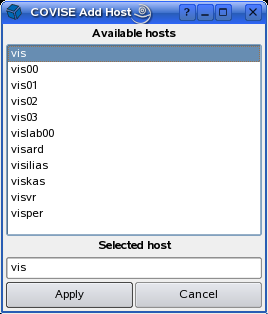
\includegraphics[scale=0.5]{mapeditor/pict/addhost1}
	  \end{minipage}
	  \hspace{1cm}
	  \begin{minipage}[b]{.4\linewidth}
   	 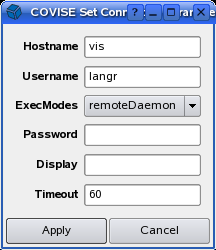
\includegraphics[scale=0.5]{mapeditor/pict/addhost2}
	  \end{minipage}
	  \caption{Adding hosts for distributed or dollaborative working mode}
	  \label{fighost}
	  \end{figure}
	  \endlatexonly

	 \end{itemize}

	 The timeout value specifies how many seconds a process will wait to be contacted by a new process
	 it initiated (e.g the Controller waiting for module). This parameter should be increased if the  network is slow.

	 The execeution mode specifies the command which should be used to start the {\bf CRB} 
	 on the remote computer. Possible execution modes are:

	 \begin{itemize}
	 \item {\bf rexec}

	 An userid and a password for the remote machine has to be typed. This is similar to login 
	 on a remote computer via telnet.

	 \item {\bf rsh}

	 In this case only the userid is required. A password on the remote machine is not needed. The rsh specific 
    rules for remote execution pf proceses have to be followed.

	 \item {\bf ssh}

	 Same as above, but a secure shell is needed. 

	 \item {\bf nqs}

	 This is not recommended. It can be used to put the {\bf CRB} into a batch queue.

	 \item {\bf manual} 

	 Manual means that someone has to start the {\bf CRB} process manually on the remote machine.
	 This can be useful for sessions across firewalls or access to the remote account is not available.
	 In this mode {\bf COVISE} writes a message in the window  \\
	 \verb/start "crb 31005 129.69.29.12 1005" on visper.hlrs.de/ . \\
	 The collaborativg partner has to type in this quoted string. 
    
	 \item {\bf remoteDamon} 

	 A remote {\bf COVISE} daemon has to run on the other machine. Currently this is only avalaible for Windows. 
    
	 \end{itemize}

	 When the remote host is successfully added, the remote username and hostname will appear 
    in the ist of hostnames of the {\mymodulebrowser} with a different color. 
 
 
 

	 \subsection{Module Menu}
    \label{modulemenu}
	 
	 Module icons in the {\mycanvas} can be manipulated.

	 \addimage{menumodule}
	 \addpict{0.5}{mapeditor/pict/menumodule}{Module Menu}{figmenuemodule}  

	 The settings are:

	 \begin{itemize}
	 \item {\bf Select all} 

	 All modules in the canvas are selected. Further operations can be applied on this group. 
    

	 \item {\bf Delete selected} 

	 Delete currently selected modules. 

	 \item {\bf Search modules...} 
    
    This entry opens a window which allows to enter a search string. All categories and/or modules containing 
    this string in the name will be highlighted. Icons of these module in the {\mycanvas} will also be highlighted.
	  
	 \addimage{search2}
	 \addpict{0.4}{mapeditor/pict/search2}{List of categories/modules after search operation}{figmenuesearch}  

	 \end{itemize}


   \clearpage
   

	 \subsection{Tools Menu}
    \label{toolmenu}

	 The items of this menu entry open additional window parts.
	 

	 \addimage{menutools}
	 \addpict{0.5}{mapeditor/pict/menutools}{Tools Menu}{figmenuexec}  

	 The settings are:

	 \begin{itemize}
	 \item {\bf Control Panel} 

	 Enables/disables an additional window on the right side. 
    
	 \addimage{mapeditor_with_cp}
	 \addpict{0.4}{mapeditor/pict/mapeditor_with_cp}{\mapeditor with Control Panel}{figmenumapcp}  
    
    \latex{More information about the {\bf Control Panel} is available in section \ref{control}.}
    \html{\htmlref{Control Panel}{control} shows more information.}
    

	 \item {\bf Data Viewer} 

	 Opens an additonal window containing the {\covise} {\mydataviewer} . 

	 \end{itemize}









	 \section{Available Help}
	 \label{help}


	 \subsection{Tooltips}
	 \label{tooltips}


	 A tooltip is a small piece of text that appears  when the cursor is hover a widget for a certain period of time.
    Tooltips are available for all icons of the {\mytoolbar}, the main buttons in the {\myparameter} window,   
	 the {\mycontrol}, the {\mysetting} and some other relevant items. 
    
    
	 \subsection{What's this ?}
	 \label{whatsthis}

    If more information is needed about a certain region of the {\mapeditor} the "What's This ?" mode is ideal. 
    The mode can be entered when the ? icon in the  {\mytoolbar} is clicked. The cursor changes to *** . Click a region 
    to obtain more information.
    
    
    \subsection{Online help}
    
    {\covise} opens a seperate help window when the item "Help" in the menubar is pressed. 
    This window is also available with \verb:Shift+F1:.
     
	 \addimage{menuhelp}
	 \addpict{0.5}{mapeditor/pict/menuhelp}{Available help items in the menubar}{figmenuhelp2_} 

	 The following help topics are available.

	 \begin{itemize}
	 \item {\bf Version} 
	 shows the version of your {\covise} installation. 
    
    \item {\bf Tutorial}
	 opens the online version of the Tutorial 

  	 \item {\bf User Guide} 
	 opens the online version of the User Guide

  	 \item {\bf Module Reference Guide} 
	 opens the online version of the Module Reference Guide
	 	 
	 \item {\bf Programming Guide} 
	 opens the online version of the Programming Guide 
	 
	 \end{itemize}





	 \section{Toolbar}
	 \label{toolbar}


	 The {\bf Toolbar} contains  
	 
	 \begin{enumerate}
	 \item icons for the most important actions
	 \item frequently used modules 
	 \end{enumerate}
	 
    
    
    
    
	 
	 \subsection{Toolbar Icons}

	 \addimage{toolicons} or   \addimage{toolbar2}
	 
    
	  \latexonly
	  \begin{figure}[!htbp]
	  \hspace{3cm}
	  \begin{minipage}[b]{.4\linewidth}
   	 
\includegraphics[scale=0.5]{mapeditor/pict/toolicons}
	  \end{minipage}
	  \hspace{1cm}
	  \begin{minipage}[b]{.4\linewidth}
   	 
\includegraphics[scale=0.5]{mapeditor/pict/toolbar2}
	  \end{minipage}
	  \caption{Available icons in the toolbar}
	  \label{figtoolicons}
	  \end{figure}
	  \endlatexonly
	  
	 These icons have the same behaviour as the items in the {\mymenubar}. The toolbar is dockable that means it can be 
    disconnect from the main window and show the content in an own separate window. A short decription
	 of the icons is given in the following list:

	 \begin{enumerate}
	 \item Load a new map into {\bf COVISE}
	 \item Save the current map. Overrides a given map name !!
	 \item Execute the module network 
	 \item The "What's This" help cursor 
	 \item Request the master state (only enabled if you are in slave mode) 
	 \end{enumerate}





    \subsection{Favourites}

    Favourites are often used modules. They can be used in the same manner as modules listed in the \mymodulebrowser.
	 
	 \addimage{favorites}
	 \addpict{0.5}{mapeditor/pict/favorites}{Frequently used modules}{figfavourites} 
    
    
	 \begin{enumerate}
	 \item The module name can be dragged into the {\mycanvas}. 
	 \item New favourite can be addeed to the list by dragging a module from the {\mymodulebrowser} to the favourite list. The drop 
    point marks the position in the list. 
	 \item A favourite can be removed from the list by dragging a favourite name to the {\mymodulebrowser} window. 
	 \item The list can be sorted by double clicking on a favourite name.
	 \end{enumerate}
	 

%\clearpage

	 \section{Module Browser}
	 \label{modulebrowser}

	 This area contains a hierarchy (tree) displaying the hostnames, category names and module names. When {\bf COVISE} is 
    started in single user mode only the name of the local host is shown in the tree. 
    
    \addimage{browser} 
	 \addpict{0.5}{mapeditor/pict/browser}{Parts of the Module Browser}{figbrowser} 
    
	 Modules running on a host appear in the same color as the host name in the list. The 
	 subdirectories of \verb+ ~/covise/ARCHSUFFIX/bin+ will be used as names of the categories. The files 
    in each category subdirectory are displayed as module names.  
    
    Short description of the category and the modules are shown as tooltips. Clicking on a 
    host with the right mouse button opens a popup menu with one single entry {\it Delete Host}. Clicking on this 
    item with the left mouse button will remove all modules running on that host and a possible 
    remote user interface. Clicking on a category or module with the right mouse button will open the {\bf COVISE} help system. 
    
    The modules shown for each category depend on the choosen modules in former sessions. To simplify the view 
    only modules which have been used before are shown. All other modules are hidden 
    behind the item {\it More..}. Clicking on this item will show all available modules in this category.
    
    The special category {\it All} contains all available modules in alphabetic order and the corresponding category.
   
	 \addimage{browser_all}
	 \addpict{0.5}{mapeditor/pict/browser_all}{The catgory ALL}{figbrowser1} 
    
    Interacting with the Module Browser is done in the following ways:
    
	 \begin{enumerate}
	 \item Clicking on the +/- sign open/close the corresponding category.
    \item Double clicking on a category name opens this specific category and closes all others.
    \item Clicking into the {\mycanvas} and typing / allows to enter a search string. All categories containing this string in the 
    module name will be highlighted. Icons of these module in the {\mycanvas} will also be highlighted.
	 \end{enumerate}
    
    
	 To start a module its module name has to be dragged to the canvas.  A {\myicon} on the canvas indicates, that the respective 
	 program representing the module has been started and waits for its execution. 


\clearpage
    
    
	 \section{Visual Programming Area (Canvas)}
	 \label{canvas}

	 This canvas is used to show the module network. Module icons,
	 that can be moves around, and connection lines between module ports can be seen. 
	 Executing a map visualizes the data using the {\bf Renderer} window. The execution of modules is indicated by 
	 highlighting the icon boundaries of currently executing modules. This red 
	 highlighting sweeps sequential through the processing pipeline.
    
	 \addimage{canvas}
	 \addpict{0.5}{mapeditor/pict/canvas}{The Visual Programming Area}{figcanvas} 



	 \subsection{Module Icon}
	 \label{icon}



	\latex{Fig. \ref{figicon}} \html{The above picture} shows a typically module icon. 
	 Each module is represented by such an icon. A module icon has 

	 \begin{itemize}
	 \item a background color which corresponds to the hostname color of the {\mymodulebrowser}.
    
	 \item input data ports
		 \begin{itemize}
		 \item {\bf pink}
       
       These ports have to be connected. Otherwise an error message appears.
		 \item {\bf green} 
       
       These ports can be optionally connected.
		 \end{itemize}
       
	 \item Output data ports
		 \begin{itemize}
		 \item {\bf blue}
       
       Normal output ports
		 \item {\bf orange}
       
       These output ports depend on an input port. If such an output port is selected 
		 the corresponding input ports change its color and become required. If disconnected the 
		 corresponding input port become green again.
		 \end{itemize}
       
	 \addimage{moduleicon}
	 \addpict{0.5}{mapeditor/pict/moduleicon}{Module Icon}{figicon} 
	 
	 \item a text label which consists of the module name and an instance number.
    
	 \item a book icon. If the closed book icon is selected, the {\myparameter} window of this module will be opened. 
		 In this window the module parameters are shown and can be changed. If an opened book icon is selected, the 
		 {\bf Module Parameter} window will be closed.
	 \end{itemize}



    \addimage{portinfo} 
	 \addpict{0.5}{mapeditor/pict/portinfo}{Available data types on a port}{figport1} 
    
    A tooltip shows port information like name, description and available datatypes.   
    If a data object exists (after the pipline has already been executed) information about the created
    data type are shown, otherwise the text {\it No data object} appears.



	 \subsection{Module Actions}
	 \label{actions}
    
	 A popup menu is shown, when the right mouse button is 
	 pressed on a module icon. This allows to 
	 perform the following module actions:  


	 \addimage{iconaction}
	 \addpict{0.5}{mapeditor/pict/iconaction}{Available Module Actions}{figiconaction} 


	 \begin{itemize}
	 \item {\bf Execute}

	 This executes the module network starting from the current module. It is typically 
	 more efficient to execute only a part of the map after having changed some parameters
	 instead of executing the whole network. I/O modules often need a lot of time to read in large
	 data files which is not necessary if a module parameter has been modified further 
	 down in the module chain.
	 
	 \item {\bf Delete} 

	 The module is deleted and disappears from the canvas. This function is also avaibale to remove a module group. 
	
	 \item {\bf Restart/Move} 
    
    Restarts the module with the current parameter values and connection lines.
    
    In distributed and collaborative working mode the module is moved to an other host 
    for execution. This means that the module is deleted on the current host and initialized 
	 on the other host. The current parameter and connections are moves too. This is only possible, 
	 if a further host was added.
	 
	 \item {\bf Clone/Copy} 

	 An exact copy of the module with the current parameter values is created. Connection lines 
    inside a copied module group are also picked.
    
    In distributed and collaborative working mode the module is copied to another host 
    for execution. This means that the module is initialized on the other host and remain on the original host. 
	 This is only possible, if an  additional host was added.
			
	 \item {\bf Rename}

	 The module is renamed. A new name is prompted for. This action is also avilable to add a label to a module group.
	 
	 \item {\bf Parameters} 

	 The \myparameter window is opened. This action has the same effect as clicking on a module book icon.

	 \item {\bf Help}

	 A HTML module description is shown in the Qt Help viewer, that is part of the {\mapeditor}. 

	 \end{itemize}





	 \subsection{How to move a module}

	 Hold down the left mouse button on the module icon.  The mouse pointer changes and you can move
	 the icon to a new position. The icon will follow the mouse pointer. Then release the mouse button. 
	 If the icons have connection lines to other ports, these lines will be repositioned too. 




	 \subsection{How to group modules}

	 \addimage{selectednodes}
	 \addpict{0.5}{mapeditor/pict/selectednodes}{Grouped module icons}{figselectednodes} 

	 YThere are two methods for grouping module icons on the canvas:

		 \begin{enumerate}
		 \item {\bf Specific Selection}

		 Press the SHIFT-Key and click on a module icon. The icon background changes to 
       the \html{\htmlref{user selected }{setting}} highlight color \latex{(see section \ref{setting})}. 
       Doing the same action on an already selected module icon deselects it.

		 \item {\bf Selection via a rubberband}

		 Click on an empty part of the canvas to determine the startpoint of the 
		 rubberband rectangle. Keep the mouse button pressed and move the mouse 
		 so that module icons which should be grouped together lie completely inside 
		 the rectangle. After the mouse button is released each of the icons inside the group
		 become red (the current hihglight color). Clicking on an empty part of the canvas ungroups the group. 
		 
       \item { \bf CTRL+A selects all modules on the canvas}.
		 \end{enumerate}


	


	 \subsection{Connecting Ports}
	 \label{connecting}

	 To build a module network you must connect the output ports of modules to the 
	 input ports of follow-on modules. Input and output ports of modules are 
	 color coded buttons according to the {\myicon}. A blue input 
	 port represents a data port, that has to be connected before a proper 
	 execution is possible. A green input port represents an optional port that can 
	 have a connection. Not all blue output ports need to be connected.  

    There are two methods for connecting ports:
    
    \begin{enumerate}
    \item{\bf Using the left mouse button}
    
	 The easiest way to establish proper connections without looking into 
	 the detailed descriptions of the module ports is by clicking with the left mouse 
	 button on the port of a module. This leads to  highlighting and/or blowing up of matching module ports, which 
    offer the appropriate data type. 
    
    \addimage{connect1} 
	 \addpict{0.4}{mapeditor/pict/connect1}{Generating a connection line: Image after clicking on a module port}{figiconaction} 
    
    Move the cursor to a heighlighted port. You now see a rubber line following 
    your mouse cursor. 
    
	 \addimage{connect2}
	 \addpict{0.4}{mapeditor/pict/connect2}{Generating a connection line: Move the cursor}{figiconaction2} 
    
    The connection is established when the mouse button is released within a port. 
    You can also directly click onto the the desired highlighted port. In the same 
	 way you have to connect all modules of a map.
    
	 \addimage{connect4}
	 \addpict{0.4}{mapeditor/pict/connect4}{Generating a connection line: Connection established}{figiconaction3} 


    \item{\bf Using the right mouse button}
    
	 Pressing/clicking on a port with the right mouse button pops up a menu that shows matching ports. 
    Selecting an item will create a connection line. This method is best when the network map has a lot a modules 
    some of them outside the visible range.
    
	 \addimage{connectright}
	 \addpict{0.4}{mapeditor/pict/connectright}{Generating a connection line with the right mouse button}{figiconaction4} 

    \end{enumerate}
    
    Move the mouse over a connection line. The line will be highlighted if the cursor is exactly on the 
    line. Delete the connection line by a double click or via a popupmenu that is shown 
    when using the right mouse button on a line.
    


	 %\clearpage

    
	 \section{Module Parameter}
	 \label{parameter}

	 Every module can present a detailed view of its input and output data objects 
	 as well as its parameters. Click with the left mouse button on the book icon of a module. 
    A new window appears on top of the {\bf MapEditor} window (default) or a new dockable widget becomes 
    visible inside the main {\mapeditor} window. The positions depends on your {\mysetting} parameter.

	 \addimage{moduleparameter1}
	 \addpict{0.5}{mapeditor/pict/moduleparameter1}{Module Parameter Window}{figmoduleparameter} 

	 Each parameter is represented  by 

	 \begin{itemize}
	 \item {\bf Name} 

	 This toggle button is used to map an interactor to 
	 the {\mycontrol} window. It contains also the name of the parameter. The type (
    {\it String, Boolean, Vector, Scalar, Slider, Choice, Browser}) and the description is shown as tooltip. 
    Most of the parameters were mapped with a standard appeareance that cannot be changed.

	 \item {\bf Appearance} 

	 Different appearance types for the parameter can be used {\it Scalar} and {\it Slider}. It is always
    possible to change the type.
     
    For the parameter type {\it Brower} and {\it Colormap} a folder icon is visible. Clicking on this icon 
    opens an additional browser window either below the parameter list inside the {\bf Module Parameter} window 
    or in a seperate window. Clicking on the open file icon will close the browser window.

	 \item{\bf Values} 

	 The value fields contain the parameter values. Depending on the parameter type different 
	 input fields to change the values are available. Values can be selectively overwritten . 
    The following list will show the different represenation of the parameter types

	 \begin{description}
	 \item[String] 
	 Just type in a string in a text input field.

	 \item[Boolean]
	 A toggle button is shown. Click on it to set/unset the state.
    
	 \item[Vector]
	 For each element of the vector a short text field is given which is used
	 as a string input field    

	 \item[Choice]
	 A combo box with the current item is shown. Click on the arrow to see all items.

	 \item[Scalar]
	 There are integer and float scalar parameters available. In the parameter window both are handled 
    in the same way. There are a text input field for the current value and one for a delta value. 
    The last value is only estimated. Please adapt this value. It is used by the interactors 
    to calculate a new current value.

	 \item[Slider]
	 Slider parameters are values that have a minimum and a maximum value, to be used to step up and down 
	 endless as a scalar parameter. They also have a delta value assigned that is used by the interactors.    
        
	 \item[Browser]
	 To choose a filename together with the proper path use either a string input field or 
	 a filebrowser. The first alternative is useful if the path and the 
	 filename is already known, otherwise open the file browser to find the file.	
    Depending on the settings the file browser 
    is opened in a seperate top level window or inside the {\bf Module Parameter} window.  
    
	 \addimage{filebrowser_in}
	 \addpict{0.4}{mapeditor/pict/filebrowser_in}{File Browser inside the Module Parameter window}{}
        
	 \item[Colormap]
	 How to modify a colormap is explained in {\mycolormap}.

    
	 \end{description}
	 \end{itemize}

   \clearpage
   
    
	 \section{Control Panel}
	 \label{control}

	 The purpose of the {\bf Control Panel} is the collection of graphical interactors which typically represent 
	 often used and changed parameters. 

    
	 \addimage{controlpanel1}
	 \addpict{0.5}{mapeditor/pict/controlpanel1}{Control Panel Window}{figcontrol}
	

	 Widgets corresponding to the parameter types are used for the layout of interactor. Interactors in the {\bf ControlPanel}  
	 allow the manipulation of parameters at every time without the need to 
	 pop up the {\myparameter}. By clicking the toggle button in the 
	 {\bf Module Parameter} window an interactor is generated. Its representation then appears in the 
	 {\bf Control Panel}.  

	 Changes made via interactors in the {\mycontrol} are updated in the 
	 corresponding parameter value fields of the {\myparameter} window.  This works also vice versa. 

	 Available interactors for each parameter are shown in the following list.

	 \begin{itemize}
	 \item {\bf String}
	 Only one string interactor is available. Just type in a string in a text input field.

	 \item {\bf Boolean}
	 A boolean interactor is realized as a toggle button. Click on it to set/unset the state.
	 This is the only one.

	 \item {\bf Vector}
	 A vector interactor has the same text input fields as in the {\myparameter} window. This is the default.	

	 \item  {\bf Choice}
	 As in the {\myparameter} window you see a combo box.  

	 \item {\bf Scalar}

	 \begin{itemize}
    
 			\item {\bf Scalar interactor = default}	This interactor has the same input fields as in the
			{\bf Module Parameter} window.

 			\item {\bf Sequencer interactor}	 Use this interactor like the control element of a
			videoplayer. There are no limits for the upper and lower value.
         
	 \end{itemize}	
    
	 \item {\bf Slider}
    
	 \begin{itemize}
 			\item {\bf Slider interactor = default}	

 			\item {\bf Player interactor}	Use this interactor like the control elements of a
			videoplayer. Keep in mind that the value has a range.		
         
	 \end{itemize}		
		
	 \item  {\bf Colormap}
	 This interactor works the same way as in the {\myparameter} window. Open/close a 
	 filebrowser if necessary.

	 \item  {\bf Browser}
	 This interactor works the same way as in the {\myparameter} window. Ppen/close a 
	 filebrowser if necessary.
     
	 \end{itemize}





	 \section{Data Objects, Data Viewer}
	 \label{data:viewer}

	 Data objects are created when a map is executed. The names of the data 
	 objects are generated generically, after the map was executed once. After a 
	 new execution the list is updated with the new names. 
    
    If you select a data object in the {\bf Data Object Browser}  more information is shown in the {\mydataviewer}
    on the right side of the {\mapeditor} 

	 \addimage{dataviewer}
	 \addpict{0.5}{mapeditor/pict/dataviewer}{Explore a COVISE Data Objects}{figdataviewer}
	 

	 Be careful if the data field is large or the data is located on another host, 
	 because this action will be time consuming.  

%\clearpage

	 \section{Colormap Editor}
    \label{colormap}

	 \addimage{colormap}
	 \addpict{0.5}{mapeditor/pict/colormap}{The Colormap Editor}{figcolormap}

         The purpose of the colormap editor is to define the ``transfer
         function'', i.~e.\ the mapping from scalar values to opacity
         (i.~e.\ inverse transparency) and colour values.
         The range of your data is mapped to $[0, 1]$ for the purpose of
         defining colour mappings.

         The transfer function is given as a piecewise linear mapping,
         the small triangles (``interpolation markers'') below the coloured bar
         in the picture above serve as nodes for linear interpolation.
         By clicking on an interpolation marker you can select it for
         manipulation:
         \begin{itemize}
         \item change its position by dragging it or by entering a new
         value in the input field labelled ``Current'', 
         \item modify colour and opacity -- this is described in
         more detail below.
         \end{itemize}

         The opacity can be modified by the self-named slider and input
         fields.
         For changing the colour values, there are more possibilities:
         \begin{itemize}
         \item enter red/green/blue values (in the range from $0$ to
               $1$) in the corresponding input fields,
         \item modify the colour according to the
         hue/saturation/value space: choose a colour hue and saturation in the large square
         and select the value in the coloured slider to the left of the
         large rectangular region, where the current colour is displayed,
         \item specify numerically hue, saturation and value in the
         corresponding input fields.
         \end{itemize}
         The resulting colour map is displayed in the large bar near the
         bottom.

         For speeding up, chose from predefined
         colour maps available in the configuration file with the
         ``Available Colormaps'' combo box, use the button labelled
         ``Save in ConfigFile'' for adding such a colour map.


%\clearpage
	
	 \section{Settings}
    \label{setting}

	 \addimage{settings}
	 \addpict{0.5}{mapeditor/pict/settings}{Settings for the Map Editor}{figsetting}

   Settings are used for the appearance and behaviour of the {\mapeditor}. These parameters are stored in the 
   file {\it mapqt.xml} which resides in \verb+$HOME/.covise+ and in \verb+$APPDATA\covise+ respectively.
   
   \begin{itemize}
   
   \item{\bf QT style (default)}
   
   defines the Qt theme used for the layout. These themes can differ from one operating system 
   to the other. On Linux systems the default style is used.
   
   \item{\bf Expert Mode (off)}
   
   If set all modules in the {\mymodulebrowser} are always shown.
   
   \item{\bf Auto connect hosts (on)}
   
   Autoconnect hosts of a loaded network if this map contains additional hosts.
   
   \item{\bf Embedded Filebrowser (on)}
   
   Opens the filebrowser for this module parameter inside the {\myparameter} window.
   
   \item{\bf Embedded OpenSG Renderer (off)}
   
   Integrate the OpenSG renderer windows inside the {\mapeditor} as a tab on the right side. Currently not implemented.
   
   \item{\bf Restore window layout (on)}
   
   After quitting the {\mapeditor} all positions and sizes of all windows are stored and reopened again the next time. 
   
   \item{\bf Error dialog boxes (off)}
   
   Off - show errors in the {\mymessagearea}. \\
   On  - pops up a dialog error window.
   
   \item{\bf User configuration path (~/.covise) }
   
   Path for storing files.
   
   \item{\bf Module History Length (50)}
   
   Maximal numbesr of modules that will be stored.
   
   \item{\bf Autosave file name (autosavemap.net)}
   
   After a certain amount of time a map is automatically stored using the above name.
   
   \item{\bf Autosave interval (120)}
   
   After a certain amount of time (120 sec) a map is automatically stored.
   
   \item{\bf Highlight module ports (on)}
   
   When connecting ports in the {\mycanvas} highlight matching ports.
   
   \item{\bf Highlight color (red)}
   
   Color name (from rgb.txt) for highlighting ports, connection lines and module icons.
   
   \item{\bf Enlarge module ports (on)}
   
   When connecting ports in the {\mycanvas} blow up module ports for better visibility .
   
   \item{\bf Enlarged port size (15)}
   
   Hight of enlarged module ports in pixel.
   
   \item{\bf Axis aligned connections (off)}
   
   When moving module icons in the {\mycanvas} the move of corresponding connection lines were shown (time comsuming)
   
   
   \end{itemize}



	
	 \section{Message Area}
    \label{message}

	 \addimage{message}
	 \addpict{0.5}{mapeditor/pict/message}{Message Area}{figmessage}

	 This scrollable text output window shows messages with different colors
	 \begin{itemize}
	 \item Error message are colored red.
	 \item Warning message are colored blue.
	 \item Info message are colored green.
	 \item Informations and control output produced by the {\mapeditor} itself are black.
	 \end{itemize}
    
	 Messages are sent from modules during their execution, the {\bf Controller} and the 
    request broker {\bf CRB}.





	 \section{Chat Line}
    \label{chat}


	 This editable text field is used for sending information to other partners joining a {\bf COVISE}  
    session. As expected, the chat line is shown for two or more partners only.  
    
			% using the mapeditor (Ruth Lang)	

\begin{htmlonly}


\usepackage{html, htmllist}
\usepackage{longtable}

\bodytext{bgcolor="#ffffff" link="#0033cc" vlink="#0033cc"}

%%%==================================================	
%%%==================================================	

% #1  mark defined by \label
% #2  a linktext 
% #3  a html link 
\newcommand{covlink}[3]{\htmladdnormallink{#2}{#3} \latex{(\ref{#1})} }


\newenvironment{covimg}[4]%
{
 \begin{figure}[htp]
  \begin{center}
   \latexonly
      \includegraphics[scale=#4]{#1/pict/#2}
   \endlatexonly  
   \html{\htmladdimg[align="center"]{pict/#2.png}}
   \caption{#3}
  \end{center}
 \end{figure} 
}{} 

\newenvironment{covimg2}[3]%
{ 
 \begin{figure}[htp]
  \begin{center}
     \latexonly
       \includegraphics[scale=#3]{#1/pict/#2}   
     \endlatexonly
     \html{\htmladdimg[align="center"]{pict/#2.png}}
  \end{center}
 \end{figure} 
}{}

\definecolor{output}{rgb}{0.,0.,1.}
\definecolor{depend}{rgb}{1.,0.65,0.}
\definecolor{required}{rgb}{0.58,0.,0.83}
\definecolor{optional}{rgb}{0.,0.39,0.}

\newcommand{\addimage}[1] {\html{\htmladdimg{pict/#1.png}}}

\newcommand{\addpict}[4] {\latexonly
	     \begin{figure}[!htbp]
			  \begin{center}
   	 		  \includegraphics[scale=#1]{#2}
   	 		  \caption{#3}
		 		  \label{#4}
			  \end{center}
	 		\end{figure}
	     \endlatexonly}



\newcommand{\mapeditor}{\textbf{Map Editor}}
\newcommand{\covise}{\textbf{COVISE}}


\end{htmlonly}


%=============================================================
\startdocument
\chapter{COVER}
\label{COVER}
%=============================================================

COVER (COvise Virtual Environment Renderer) is a COVISE renderer module
with support for Virtual Reality (VR) input devices, backprojection displays,
and intuitive interaction. 
COVER can also be started independendly of COVISE and just be used as a virtual
reality viewer for 3D geometry.

To start COVER within COVISE, select the module COVER in the module list
under the category Renderer.

To start COVER as a 3D viewer, type in 
\begin{verbatim}
    cover <filename>
\end{verbatim}

{\it Note: Please make sure to set the variable DISPLAY in your environment before starting
COVER!}

COVER is based on Performer, a high level 3D graphics library from
SGI, providing high speed rendering, multi-processing, multi-pipe,
scene graph, loaders for 3D database formats...
Performer is available for IRIX and Linux platforms.

This chapter about COVER describes the {\large {\bf COVER User Interface}} and 
has the two sections:

\begin{itemize}
\item \html{\htmladdnormallink{Interaction in COVER}{Interaction.html}}\latex{{\bf Interaction in COVER}
(\ref{label_chapter_interaction})}:
This section describes how to use COVER. It explains the entries in the 3D menu and the corresponding interaction techniques. 
\item  \html{\htmladdnormallink{PlugIns}{Plug_Ins.html}} \latex{{\bf PlugIns}
(\ref{Plug_Ins})}:
This section describes the plugins "Probe" and "Viewpoints".
\end{itemize}

For configuration of displays and input devices see the separate document \newline

 {\it COVER Installation and Configuration}\newline

with the sections

\begin{itemize}
\item {\bf Graphics Board and Display}: 
This section explains which types of Virtual Environments are supported and how to configure COVER and your graphics workstation for this Virtual Environment.
\item {\bf Input Devices}: This section explains which types of Virtual Environments are supported and how
to configure COVER and your graphics workstation for this Virtual Environment.
\end{itemize}

%\item[\html{\htmladdnormallink{Graphics Board and Display}{Graphics_Board_Display.html}}
%\latex{{Graphics Board and Display } (\ref{label_chapter_display})}]
%This section explains which
%types of Virtual Environments are supported and how
%to configure COVER and your graphics workstation for this Virtual Environment.

%\item[\html{\htmladdnormallink{Input Devices}{Input_Devices.html}}
%\latex{{Input Devices} (\ref{label_chapter_input})}]
%This section explains which
%3D input and tracking devices are supported and how to configure 
%COVER for your specific devices.

%\newpage
%\input cover/display/display 
%\newpage
%\input cover/input/input


\section{Interaction}
\label{label_chapter_interaction}

COVER can be used either as a viewer for 3D scenes or as a renderer
module in COVISE.

As a 3D viewer COVER supports all 3D file formats which are also supported by the 
graphics library OpenGL Performer and additionally vrml files with 
sound and interaction. To load a specific file call COVER with the file 
name as parameter:
\begin{samepage}
\begin{verbatim}
    cover <filename>
\end{verbatim}
\end{samepage}


As a COVISE renderer module COVER is started through the Mapditor. Select the category renderer
and drag the module COVER to the map area. You can now connect all modules
to COVER which generate geometric primitives like lines, triangle strips, 
polygons or points with colors, normals and textures.

\begin{covimg}{cover}{renderer_start}{Starting COVER as COVISE Renderer Module}{0.7}\end{covimg}

If you have a full COVISE installation you will recognize that there
are two COVERs: one called COVER and one called COVER\_VRML. Only the
second one supports vrml files with sound and interaction. As you don't
need this functionality for most COVISE visualisations, a smaller 
version without vrml support, named COVER, is provided, too.

\label{label_tracking_3dpointer}
\subsection{Headtracking and 3D Pointer}
In COVER the user can freely move in the virtual scene  
and manipulate it with a 3D input device.

The movement of the user is measured with a sensor 
mounted at the glasses. With the measured position and orientation an 
appropriate view on the scene is computed. This is called head tracking.
Currently only one user can be tracked. Other users don't have the correct 
view of the scene and therefore they have the impression that all objects 
are slightly distorted. This effect is minimized if they try to stand close 
to the user with the tracked glasses and try to look into the same 
direction as the one with the tracked glasses. 

The location and orientation of the 3D input device, which the user
holds in his hand, is measured through a sensor in the input device.
The input device usually has one two three buttons. One button is 
used to indicate a selection. On a three button device the other two buttons
are used to switch the navigation mode without using the 3D menu.

With the virtual laser beam which seems to come out of the 3D input device also
remote objects can be reached, for example buttons in the 3D menu.

\begin{covimg}{cover}{menu_selection}{Selecting a menu entry with the laser beam}{0.7}\end{covimg}

\subsubsection{Using COVER with the mouse}
COVER can also be used with the mouse. The viewer position is then fixed to
the position defined in covise.config:
\begin{samepage}
\begin{verbatim}
COVERConfig
{
    ...
    TRACKING_SYSTEM MOUSE
    VIEWER_POSITION  <x> <y> <z>
    ...
}
\end{verbatim}
\end{samepage}



The interaction possibilities with the menu and the 3D scene are described
in the following chapters.

\label{label_chapter_stereo}
\subsection{Stereo Viewing}

For the stereo projection two images are generated, one with the perspective
of the right eye and one with the perspective of the left eye. The stereo
glasses show only the appropriate image to each eye. Like stereo viewing
in reality the brain forms a 3D impression of the scene.

And similar to reality objects which are very close to the users head
are seens twice because the two images can't be fused any more, objects
which are very far don't appear to be three dimensional but flat.
Therefore the optimal location of obejcts for stereo viewing are not too
near and not too far. 

If the scene size fits into the virtual reality
environment, the best position is near the front screen, optimally one part
of the scene is in front of the screen and the other part behind. 
For many technical visualisations for example flow visualisation of
the air around a car the scene can be scaled so that it fits into the
virtual environment (see chapter xy view all).

Larges scenes like landscapes are best viewed on large screens.
If the scene is larger than the screens, but the screen is so small that it 
is inside the users field of view the stereo impression can get lost, 
when the object is located in  front of the screen. 
This happens because the human brain is so used to the fact that in reality
objects partly covered by something are behind that it can't form a stereo 
impression if a virtual scene is cut by the frame of the screen. 
Therefore for large scenes and small screens  the best position is behind 
the screen and the screens is like a window to the outside.

\label{label_chapter_3dmenu}

\subsection{3D Menu}

The navigation mode, viewing options, and manipulation modes are
selected through a 3D menue, called the Pinboard. You select a menu entry
by pointing to the button with the laser beam and pressing the 
button of the 3D input device. If the pinboard is used with a mouse
simply bring the mouse pointer over the menu entry and click a button.

The COVER Pinboard can be re-positioned in the VE by pointing to the title bar
and pressing the button of the 3D input device.If you have a 3-button device
and select it the left button, the menu is rotated around it's z axis so it 
always faces the viewer (billboard mode). Selected with the right button, it moves as if it's
mouned at the laser beam. Selected with the middle mouse button
it changes it's size according to the rotation of the users arm. 

The same applies for mouse input: left mouse button moves the menu in a 
way that it faces the viewer, right mouse button moves the menu with the
mouse pointer. The orientation is defined through a line from the viewer
to the mouse so it seems to face the viewer, too. Middle mouse button
scales the menu, movements up and down make the menu larger and smaller. 

For one-button devices the billboard mode and the scaling is not supported.


\begin{covimg}{cover}{drag}{Menu Positioning}{0.5}\end{covimg}

The initial position, orientation, size, layout of the menu and the start 
values of toggleand group buttons can be specified in the file covise.config
(see configuration in cover installation guide).

\subsubsection{Menu Button Types}

In the 3D menu there are three different types of buttons.

\paragraph{Simple Buttons} with only a label execute a certain function once, for example
if you press the "view all"  button , the scene is scaled once so that 
it fits onto the screen.

\paragraph{Toggle buttons} 
\latexonly

\includegraphics[scale=0.5]{cover/pict/toggle_button_icon} 
\endlatexonly
\html{\htmladdimg[ALIGN=TOP]{pict/toggle_button_icon.png}}
switch between two states, for example you can
switch headtracking on or off.


\paragraph{Radio buttons} 
\latexonly

\includegraphics[scale=0.5]{cover/pict/radio_button_icon} 
\endlatexonly
\html{\htmladdimg[SCALE=0.5 ALIGN=TOP]{pict/radio_button_icon.png}}
select one function in a group of functions.
All navigation functions are in such a button group, if you you have 
"move world" on and then switch to "scale world" the "move world" button 
is switched off. 
All collaborative working modes are also in a separate button group.
Group buttons can be spread across the menu and the submenus.

\paragraph{Slider buttons} 
\latexonly
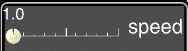
\includegraphics[scale=0.5]{cover/pict/slider_button} 
\endlatexonly
\html{\htmladdimg[ALIGN=TOP]{pict/slider_button.png}}
are used to select a numerical value between a minimum
and a maximum value. The "drive speed" button is such a slider button.
Currently only floating value slider buttons are implemented.

\paragraph{Submenu buttons} open a new menu. The submenu can be selected
and dragged like the pinboard.

\begin{covimg}{cover}{submenu_button}{Submenu Button}{0.5}\end{covimg}


	
\subsection{Navigation Modes}
With the functions XFORM, SCALE, FLY, DRIVE, WALK
the user navigates through the scene. These functions are grouped into
a radio button group, therefore only one navigation mode can be active.

\subsubsection{Move World (XFORM)}
\latexonly
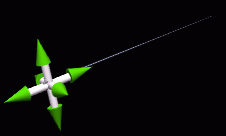
\includegraphics[scale=0.5]{cover/pict/xform} 
\endlatexonly
\html{\htmladdimg[ALIGN=TOP]{pict/xform.png}}

In XFORM mode (XFORM stands for transform) the whole scene 
(besides the coordinate axis and the pinboard) can be moved. 
The default button label is "move world" and
the default button location is in the main Pinboard menue. 
The XFORM mode indicated with the above 3D icon.

Only when the button of the 3D input device is pressed, the world
is translated and rotated with the users hand. The translation is relative 
to the point where the button was pressed. The center of rotation is the users
hand. The interaction is stopped when the button is released. For pulling
the whole scene closer to the user you can move the hand away from the body, 
then press the button and move the hand closer too th body, and then relase 
the button. Do this several times if the appropriate position can't be 
reached in one step. 

If the input device is the mouse, the scene is rotated when the left
mouse button is pressed and translated when the middle mouse button
is pressed. In rotate mode, up/down movements rotate around the x axis, 
left/right movements rotate around the z axis. In translate mode, up/down
movements translate into positive and negative z direction, left/right movements 
into positive/negative x axis.
		
\subsubsection{Scale World (SCALE)}
\latexonly
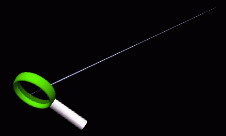
\includegraphics[scale=0.5]{cover/pict/scale} 
\endlatexonly
\html{\htmladdimg[ALIGN=TOP]{pict/scale.png}}

In SCALE mode the whole scene (besides the coordinate axis and the pinboard) 
can be scaled. 
The default button label is "scale world" and
the default button location is in the main Pinboard menue. 
The button belongs to the button group "Navigation".
The SCALE mode indicated with a magnifying class as 3D icon.

When the button of the 3D input device is pressed and the hand is
moved to he right, the world becomes larger, when the hand is moved
to the left, the world becomes smaller. The interaction is stopped when the
button is released.

The same applies for mouse input.
 		
\subsubsection{View All (VIEW\_ALL)}

When the VIEW\_ALL button is pressed, the whole scene 
(besides the coordinate axis and the pinboard) 
is scaled so that it fits into the visible part of the world - 
typically the screen size. 
The default button label is "view all" and
the default button location is in the main Pinboard menue. 
The button is a function button.

The size for the scaling is defined in the file covise.config in 
the section COVERConfig
with the keyword SZENE\_SIZE. It is defined in mm. A 19'' Monitor for
example has 340 x 270 mm, there a good choice would be 270, in a 
CAVE with the wall size 2800 x 2500 mm we would choose 2500.

\begin{samepage}
\begin{verbatim}
COVERConfig
{
    ...
    SCENE_SIZE <size in mm>
    ...
}
\end{verbatim}
\end{samepage}

COVER also supports an "autoscale" mode. In this mode a "view all" is performed
every time a new object is appended to the scene graph. You enable
this mode in the scope COVERConfig with the keyword SCALE\_ALL.
\begin{verbatim}
COVERConfig
{
    ...
    SCALE_ALL <ON or OFF>
    ...
}
\end{verbatim}

		
\subsubsection{Stop Headtracking (FREEZE)}
With FREEZE headtracking is enabled/disabled. 
The default button label is "headtracking" and
the default button location is in the main Pinboard menue. 
The button is a toggle button. The default state is 
OFF, this means headtracking is enabled. 

Freezing the current view can be useful for demonstrations with many 
people, where it is
impossible, that all users move with the demonstrator. Or for taking
pictures or making a video. There you get the best results when the
camera position matches the viewer position. In some configurations
the camera must be in the area where the magnetic tracking system doesn't
deliver correct values. Then you can freeze headtracking at starting time and
specify a viewer position:

\begin{verbatim}
COVERConfig
{
    ...
    FREEZE ON
    VIEWER_POSITION 	0 -3000 500
    ...
}
\end{verbatim}
This means for example the viewpoint is 3 m in negative y direction and
50 cm above the origin in z direction. The Performer coordinate system is
x=RIGHT, z=UP, and Y=into the screen.

		
\subsubsection{FLY}
\latexonly
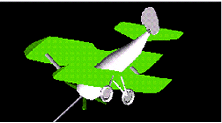
\includegraphics[scale=0.5]{cover/pict/fly} 
\endlatexonly
\html{\htmladdimg[ALIGN=TOP]{pict/fly.png}}

In FLY mode the whole scene (besides the coordinate axis and the pinboard) 
is moved as if the user sits in an airplane. 
The default button label is "fly" and
the default button location is in the "Navigation" submenu. 
The button belongs to the button group "Navigation".
The FLY mode indicated with an airplane as 3D icon.

You start the fly mode by pressing the button of the 3D input device
and then moving the hand into the direction you want to fly.
Moving the hand far away from the point where you pressed the button 
results in faster flying. Moving the hand close to the body behind the point
where you pressed the button, results in flying backwards.
A scale factor for the fly speed can be applied with the slider "SPEED".

Mouse input in fly mode doesn't work.		
\subsubsection{WALK}
\latexonly

\includegraphics[scale=0.5]{cover/pict/walk} 
\endlatexonly
\html{\htmladdimg[ALIGN=TOP]{pict/walk.png}}

In WALK mode the whole scene (besides the coordinate axis and the pinboard) 
is moved as if the user walks in the scene. 
The default button label is "walk" and
the default button location is in the "Navigation" submenu. 
The button belongs to the button group "Navigation".
The WALK mode is indicated with shoes as 3D icon.

You start the walk mode by pressing the button of the 3D input device
and then moving the hand into the direction you want to walk. COVER
then intersects a line from the feet into the negative z direction (towards the
bottom) with the scene and if close enough, repositions the user on that
point in the scene. 
As the feet are not tracked, the feet position is calculated from the
head position  and the floorHeight and the stepSize. FloorHeight and stepSize
are specified in the section COVERConfig in the file covise.config.
\begin{verbatim}
COVERConfig
{
    ...
    floorHeight <z position of the floor in mm>
    stepSize <step length in mm>
    ...
}
\end{verbatim}
	

When using a mouse for input, pressing the left button and moving the mouse
up, down, left right moves forward/backward,left and right.

\subsubsection{DRIVE}
\latexonly
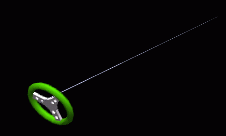
\includegraphics[scale=0.5]{cover/pict/drive} 
\endlatexonly
\html{\htmladdimg[ALIGN=TOP]{pict/drive.png}}

In DRIVE mode the whole scene (besides the coordinate axis and the pinboard) 
is moved as if the user drives in the scene. 
The default button label is "drive" and
the default button location is in the "Navigation" submenu. 
The button belongs to the button group "Navigation".
The DRIVE mode is indicated with a driving wheel as 3D icon.


\subsubsection{COLLIDE}
With COLLIDE collision detection between the viewer and the scene
is enabled/disabled.
The default button label is "collide" and
the default button location is in the "Navigation" submenu. 
The button is a toggle button. The default state is OFF.


\subsubsection{SPEED}
With SPEED you can adjust a scale factor for the velocity in fly, drive
or walk mode.
The default button label is "speed" and
the default button location is in the "Navigation" submenu. 
The button is a slider button. The default minimum speed is 1 and 
the default amximum speed is 30. The default value is 1.
The minimum and maximum and the initial value can be defined in the scope
COVERConfig:
\begin{samepage}
\begin{verbatim}
COVERConfig
{
    ...
    SPEED               <min> <max> <initial value>
    ...
}
\end{verbatim}
\end{samepage}

\subsubsection{Viewpoints}

The "viewpoints" submenu is described in the section about plugins.

\subsection{View Options}

\subsubsection{COORD\_AXIS}
With COORD\_AXIS drawing of a coordinate axis system is enabls/disabled. 
The default button label is "coord axis" and
the default button location is in the "view options" submenu. 
The button is a toggle button. The default state is OFF.

The axis are drawn as lines with a small arrow at the end. The origin
is in the world coordinate origin and the length of the axis is
0.5 * SZENE\_SIZE. The wolrd coordinate system origin is defined
in the scope ScreenConfig (see ection Display Configuration) through
the position of the screen center and the orientation of the screen. 

Typically the x axis points to the right and is drawn red, the
y axis points into the screen and is drawn green and the z axis points
up and is drawn in blue.

\subsubsection{SPECULAR}
With SPECULAR the properties of the light are changed so that objects with
a specular material appear specular.
The default button label is "specular" and
the default button location is in the "view options" submenu. 
The button is a toggle button. The default state is ON.

 
\subsubsection{SPOTLIGHT}
With SPOTLIGHT a lamp like light is attached to the users hand.
The default button label is "spotlight" and
the default button location is in the "view options" submenu. 
The button is a toggle button. The default state is OFF.
		
\subsubsection{STEREO\_SEP}
With STEREO\_SEP the offset between the left and right eye can be set
to zero.
The default button label is "stereo separation" and
the default button location is in the "view options" submenu. 
The button is a toggle button. The default state is OFF.

When STEREO\_SEP switched on, only the ofset is set to zero. The video
mode is not changed to a mono mode, so you don't have any rendering
performance advantage. Use STEREO\_SEP for example if you want to take
pictures or a video from the VE.	

\subsection{Part Manipulation}

\subsubsection{SNAP}
With SNAP constarints for the manipulation of objects are enabled/disabled.
The default button label is "snap" and
the default button location is in the "part manipulation" submenu. 
SNAP is a TOGGLE button. The default state is OFF.

Currently only the cuttingsurface and cutgeometry interaction
supports snapping. In CuttingSurface and CutGeometry 
interaction the plane orientation
is corrected to angles which are multiples of 45 degree.
 
\subsubsection{REMOVE}
In REMOVE mode objects can be selected with the pointer ray and can
removed on button press.

The default button label is "remove" and
the default button location is in the "part manipulation" submenu. 
The button belongs to the button group "Navigation".
The REMOVE mode indicated with a red pointer ray.
 
\subsubsection{UNDO}
With UNDO the REMOVE actions are undone.
The default button label is "undo" and
the default button location is in the "part manipulation" submenu. 
UNDO is a function button. To undo several remove actions, press UNDO
several times.

\subsubsection{MOVE\_PARTS}

With MOVE\_PARTS a cetrtain object can be selected and re-position/re-oriented.
The default button label is "move parts" and
the default button location is in the "part manipulation" submenu. 
The button belongs to the button group "Navigation".
In MOVE\_PARTS mode the object which is closest to the pointer ray is selected
and if the button on the 3D input device is pressed, moved with the
hand. The movement is relatively to the position where the button is pressed.
 


\subsection{Animation}
		
\subsubsection{FORWARD}

FORWARD sets the animation mode to forward playing. This means that
the objects in the animation sequence are drawn one after each other. After the
last object in the sequence it re-starts with the first object. The button appears 
only if COVER receives a COVISE set objects with timesteps.
The default button label is "forward" and
the default button location is in the "animation" submenu.  
FORWARD is a function button.


\subsubsection{Backward}
BACKWARD sets the animation mode to backward playing. This means that
the objects in the animation sequence are drawn in backwards order. After the
first object in the sequence it re-starts with the last object.
The button appears 
only if COVER receives a COVISE set objects with timesteps.
The default button label is "forward" and
the default button location is in the "animation" submenu.  
FORWARD is a function button.

\subsubsection{ANIM\_SPEED}
With ANIM\_SPEED the time interval how long an object in the sequence
is drawn, can be set.
The default button label is "anim speed" and
the default button location is in the "animation" submenu.  
FORWARD is a slider button. The minimum and maximum value and the initial
value can be defind in the scope COVERConfig:

\begin{samepage}
\begin{verbatim}
COVERConfig
{
    ...
    ANIM_SPEED               <min> <max> <initial value>
    ...
}
\end{verbatim}
\end{samepage}

The default values are min=0, max=5,0 and value=1.0.

When the slider is set to the maximum value, objects are drawn as
fast as possible. In this case a timestep containing only a few objects is drawn
faster than a timestep containing a large number of objects.


\subsubsection{Steady Cam}
With STEADY\_CAM the user can attach the viewer to an animated object and
move with this object. For example if the viewer wants to see a car crash
from the view of the person sitting in the car he can attach the camera
to the seat and then he is moved with the crashing car.
The default button label is "steady cam" and
the default button location is in the "animation" submenu.
The button belongs to the button group "Navigation".
		
		
\subsection{COVISE}

The Mapeditor function "Execute" and the parameters of the most important 
COVISE modules can be accessed from within COVER.

\subsubsection{EXECUTE}
With the function button EXECUTE the whole pipeline is eceuted once.
The default button label is "execute pipeline" and
the default button location is in the "COVISE" submenu.
		
\subsubsection{CUTTINGSURFACE}
The module CuttingSurface cuts a plane/cylinder or sphere out of a 
3D grid and interpolates the data to the plane/sphere/cylinder.
The position and orientation of the cutting surface is specified with the
parameters vertex and scalar. In the 2D interface the user has to provide
the orientation of the plane with the parameter vertex (which is the normal
on the plane) and the parameter scalar (which defines the distance from the
origin).

In COVER the user selects the button Cuttingsurface\_i, where i stands for
the instance of the module. A transparent plane is now attached to
the users hand. The plane can be positioned in the scene inside the geometry
by moving the hand to the desired position/orientation. When the Select-button
of the 3D input device is pressed, the current position/orientation is converted
to a normal and distance and sent back to the CuttingSurface module. The
CuttingSurface module is automatically executed and within a few seconds
the new cuttingsurface appears in COVER.

The default button label is "CuttingSurface i", where i is replaced
by the module instance and
the default button location is in the "COVISE" submenu.
The button belongs to the button group "Navigation", this means that if the
previos mode was a navigation mode like XFORM, this mode is switched off. 

\subsubsection{CUTGEOMETRY}
The module CutGeometry cuts a COVISE geometry with a plane.
The position and orientation of the cutting plane is specified with the
parameters vertex and scalar. In the 2D interface the user has to provide
the orientation of the plane with the parameter vertex (which is the normal
on the plane) and the parameter scalar (which defines the distance from the
origin).

In COVER the user selects the button "CutGeometry i", where i stands for
the instance of the module. A transparent plane is now attached to
the users hand. The plane can be positioned in the scene inside the geometry
by moving the hand to the desired position/orientation. When the Select-button
of the 3D input device is pressed, the current position/orientation is converted
to a normal and distance in object space and sent back to the CutGeometry module. 
The CutGeometry module is automatically executed and within a few seconds
the new cutted geometry appears in COVER.

The default button label is "CutGeometry i", where i is replaced
by the module instance and
the default button location is in the "COVISE" submenu.
The button belongs to the button group "Navigation". 
		
\subsubsection{ISOSURFACEP}
The module IsosurfaceP computes an isosurface which contains a
certain point. This point is specified with the parameter point. Then the
value at this point is computed and the all grid points, containings this
value are computed. In the 2D interface the user nters the x, y, and z coordinate
of the point in object coordinates.

In COVER the user selects "IsosurafceP i", where i stands for the instance
of the module. A red sphere is attached to the users hand. The sphere can be 
positioned in the scene by moving the hand to the desired point. 
When the Select-button
of the 3D input device is pressed, the current position is converted
to a object coordinates and sent back to the IsosurfaceP module. The
IsosurfaceP module is automatically executed and within a few seconds
the new isosurface appears in COVER.

The default button label is "IsosurfaceP i", where i is replaced
by the module instance and
the default button location is in the "COVISE" submenu.
The button belongs to the button group "Navigation". 
		
\subsubsection{Tracer}

The COVISE modules TracerUSG, MagTracer, MagBlockTracer, STracer, BlockSTracer,
CellTracer and TetraTrace all computes streamlines or particle traces.

The traces start either on a line or on a plane. In the COVISE module the
line is specified with the parameters startpoint1 and startpoint2, and the
number of traces started on that line is defined with the parameter
no\_startpoints. The plane is specified with the parameters startpoint1,
startpoint2 and normal. 
% Aber wie ?

In COVER the user selects "*Trace* i" from the Pinboard, where *Trace* stand 
for the Tracer module and i for the instance of the module. A red sphere
is now attached to the users hand. When the user presses the select-button
of the 3D input device, the current position is converted to object space
and is taken as startpoint1. The user
can move the hand now to the endpoint of the line while keeping the select-button
pressed. When he releases the button the current position is converted to object
space and is taken as startpoint2. The parameters are sent back to the tracer
module and the module is executed. Within a few seconds the new particle traces
appear in COVER.



\section{Plug Ins}
\label{Plug_Ins}


COVER provides an interface for programming Plug Ins. For details see COVISE Programming Guide,
section COVER Plugin Programming. Below you get a description of some plug ins you may find useful for
your current work.

\subsection{Probe}

{\bf Probe} is a new plugin for 2D probing. To use Probe, select first the Probe button from
the menu; a red icon will appear. If the pointer intersects a 2D object (polygon or 
triangle strips) and the button is pressed, a label will show the coordinates of the 
intersection (relative to the object) plus scalar and vector data values at that point.
The plugin reads the PROBE2D attribute(s) of the grid object which indicate the 
name(s) of the data object(s). You can configure line length and text font of the 
label, the format of the text, and a default for the kind of data to be displayed,
e.g. TEMP, in covise.config, section VRProbe:
\begin{verbatim}
VRProbe
{
   LabelLineLen 90
   LabelFontSize 7
   ScalarFormat %s= %.3f
   VectorFormat %s= %.3f  %.3f %.3f
   DefaultSpecies TEMP (e.g. - if not specified: Unknown)
}
\end{verbatim}
Additional information:
\begin{itemize}
\item don't write anything into the PROBE2D attribute
\item add the following line in the section COVERConfig 
\begin{verbatim}
             MODULE      VRProbe
\end{verbatim}
\end{itemize}
The label will be shown until a new intersection will be selected or the
Probe button will be unselected.

\subsection{Viewpoints}

A viewpoint defines the current position, orientation and scaling factor of the
scene. 
The {\bf Viewpoints} plugin allows to the user to load viewpoints from file
and save them to file ot interactively define new viewpoints. It offers a flight
through all viewpoints or activated only one selected viewpoint. 

The Viewpoint Plugin is activated if the line  
\begin{verbatim}
MODULE VRViewpoint
\end{verbatim}
in COVERConfig (as for all plugins) is available.

\subsubsection{Viewpoint Definition}

Default viewpoints can be defined in covise.config in
the section VRViewpoints, and they will be automatically inserted into the
list of viewpoints:

\begin{verbatim}
VRViewpoints
{
    1    S=1    X = 0 y=0 z=0 h=0 p=0 r=0
    10   S=10   X = 0 y=0 z=0 h=0 p=0 r=0
    100  S=100  X = 0 y=0 z=0 h=0 p=0 r=0
    1000 S=1000 X = 0 y=0 z=0 h=0 p=0 r=0
}
\end{verbatim}

In addition, and even if there is no "Viewpoints" entry in covise.config, there
is a parameter "Viewpoints" in COVER, which contains the name of a custom file
where the viewpoints are stored. If no name is indicated then the file
default.vwp will be loaded (if default.vwp doesn't exist it will be
created).
If a file is specified it will be loaded, and if it doesn't
exist, it will be created.

If COVER is started from the console, the custom viewpoints will be loaded
using  the "-v" option and the path of the .vwp file:
\begin{verbatim}
cover -v example.vwp 
\end{verbatim}


\subsubsection{The Viewpoints Menu}

The button "Viewpoints" opens a submenu with the following entries:
\begin {itemize}
\item "SaveViewPoint"
\item "Flying mode" - toggles animated flight from current to next viewpoint
\item "Flight" - opens a submenu
\item "StartRecord" - starts recording viewpoints
\item "StopRecord" - stops recording viewpoints
\item "First default viewpoint from covise.config" - if one exists
\item   ....
\item "Last viewpoint from covise.config"
\item "First viewpoint from custom viewpoint file" - if one exists
\item  ...
\item "Last viewpoint from custom viewpoint file"
\end {itemize}
By pressing "SaveViewPoint" a new entry, "NewViewpoint", will appear, and
it will be saved in the file. The name "NewViewoints" can be changed in the
file with a text editor.
By chosing a viewpoint and pressing on this entry the viewpoint will be
activated. 

If "flying mode" is active then an animated flight from the
current viewpoint to the selected viewpoint will be started. The selection of viewpoints
can also be done using the keys F1-F12.

The "Flight" button opens a submenu with a list of all viewpoints and
a button "Run". "Run" starts an automatic flight through all selected 
viewpoints in the list. Viewpoints can be removed from the flight by deselecting them 
in the list.

"StartRecord" starts recording viewoints. The viewpoints are saved in vrml
format to a file named animation.wrl. "StopRecord" stops recording viewpoints.
The recorded viewpoints have to be added to a vrml file and become available
in the submenu VrmlViewpoints, as soon as the file is loaded.

\subsection{Snapshot}

This plugin is available when an entry
\begin{verbatim}
MODULE Snapshot
\end{verbatim}
in COVERConfig is present.

When pressing the Snapshot button of the pinboard,
a submenu appears, which has a single button as long
as you have creted no snapshots. When you press this button,
the submenu disappears, and a snapshot will be creted whenever
you press the pointer again. A snapshot may encompass several rgb
files. One or two files are generated for each screen in a screen 
selection list.
By default this list reduces to screen in the first entry in the
ChannelConfig section of covise.config. You may create your own list
by adding a SNAPHOT\_SCREEN entry in section {\sl Snapshot}
of covise.config.

The rgb snapshot files are created by default in the working
directory. You may override this behaviour if a SNAPHOT\_DIR
entry in section {\sl Snapshot} is present, for instance:
\begin{verbatim}
Snapshot
{
SNAPHOT_SCREEN FRONT TOP.
SNAPHOT_DIR /usr/tmp
}
\end{verbatim}

The generated files have the following structure:\newline
snap\{number\}\_\{extra digits\}\_\{left$\mid $right\}Eye\_Screen\{Screen name\}.rgb.
The first number is a snapshot counter. The extra digits have no special
meaning, they are only used in order to prevent new file or button
names from being repeated. Whenever you create a snapshot, a new
viewpoint entry is also created for the Viewpoint plugin, which
should also be in use, otherwise the COVER will crash.
For these new viewpoints associated with snapshot actions,
new buttons are also created in the Snapshot submenu, with
the same name as in the Viewpoint submenu. These names
have the structure: snap\{number\}\_\{extra digits\}.

\subsection{Sketches}

You create drawings in 3D space using this plugin. A sketch is a set of lines.
A line is defined in this context to be a series of connected points.

The Sketches Plugin is activated if the line  
\begin{verbatim}
MODULE Sketcher
\end{verbatim}
in COVERConfig is present.

%\subsubsection{Sketch Generation}

In order to create a sketch, you should activate the {\sl Draw} button
in the {\sl Sketches} menu. Then you may create lines by pressing the
pointer and moving it. When it is released, the current line is finished.
You may create several lines by repeating this operation. When you
are done with one sketch, then you will want to create a new entry
in the list of available sketches. You should press the button {\sl NewSketch}
in this case. But this is not enough to save the sketch in a file
(see below comment on button {\sl SaveSketches}).

The available sketches may be shown or hidden by activating
or deactivating the corresponding entry in the menu.

All sketches are saved to the file specified by 
the COVER parameter {\sl Viewpoints} when you press the button
{\sl SaveSketches}, whose action will be eventually preceded
by the action of button {\sl NewSketch}. 
You may edit this file in order to change
some attributes of the sketches or their lines: sketch name,
color attributes, etc.

The position of the sketching tool with respect to the hand may
be parametrised by a pertinent section in covise.config:
\begin{verbatim}
Sketcher{
ANGLE 5.0
DISPLACEMENT 0.5
SCALE 100.0
}
\end{verbatim}
where SCALE determines the size of the sketching tool,
DISPLACEMENT stands for a displacement along the local Y axis
relative to the sketching-tool size,
and ANGLE parametrises a rotation around the local X axis in degrees.

By way of summary, you may read the table below with explanation to the
buttons in the submenu {\sl Sketches}.
%\subsubsection{The Sketches Menu}
The button {\sl Sketches...} opens a submenu with the following entries:
\begin {itemize}
\item "Draw" - enters drawing mode
\item "NewSketch" - ends the definition of a sketch and creates a new entry in the list of sketches
\item "SaveSketch" - saves all sketches to file
\item "First sketch name" - if one exists
\item "Second sketch name" - if one exists
\item   \ldots
\end {itemize}


				% using COVER (Daniela Rainer)	
\begin{htmlonly}


\usepackage{html, htmllist}
\usepackage{longtable}

\bodytext{bgcolor="#ffffff" link="#0033cc" vlink="#0033cc"}

%%%==================================================	
%%%==================================================	

% #1  mark defined by \label
% #2  a linktext 
% #3  a html link 
\newcommand{covlink}[3]{\htmladdnormallink{#2}{#3} \latex{(\ref{#1})} }


\newenvironment{covimg}[4]%
{
 \begin{figure}[htp]
  \begin{center}
   \latexonly
      \includegraphics[scale=#4]{#1/pict/#2}
   \endlatexonly  
   \html{\htmladdimg[align="center"]{pict/#2.png}}
   \caption{#3}
  \end{center}
 \end{figure} 
}{} 

\newenvironment{covimg2}[3]%
{ 
 \begin{figure}[htp]
  \begin{center}
     \latexonly
       \includegraphics[scale=#3]{#1/pict/#2}   
     \endlatexonly
     \html{\htmladdimg[align="center"]{pict/#2.png}}
  \end{center}
 \end{figure} 
}{}

\definecolor{output}{rgb}{0.,0.,1.}
\definecolor{depend}{rgb}{1.,0.65,0.}
\definecolor{required}{rgb}{0.58,0.,0.83}
\definecolor{optional}{rgb}{0.,0.39,0.}

\newcommand{\addimage}[1] {\html{\htmladdimg{pict/#1.png}}}

\newcommand{\addpict}[4] {\latexonly
	     \begin{figure}[!htbp]
			  \begin{center}
   	 		  \includegraphics[scale=#1]{#2}
   	 		  \caption{#3}
		 		  \label{#4}
			  \end{center}
	 		\end{figure}
	     \endlatexonly}



\newcommand{\mapeditor}{\textbf{Map Editor}}
\newcommand{\covise}{\textbf{COVISE}}


\end{htmlonly}



%=============================================================
%=============================================================

\startdocument
\chapter{The Renderer}
\label{Renderer}

\section{Introduction}

In this chapter the main functionality of the COVISE Renderer is summarized.
Like the map editor, one renderer is started on every host in a cooperative
working session, once the master renderer has been brought up on the master map editor. 

The design of the Renderer supports collaborative working (for more details see chapter 5,
COVISE CE - Collaborative Working): Basically the Renderer works in a 
"what you see is what I see" mode. This is called
the Master/Slave Mode or Tight Coupling. It means, that every partner in the session
has the same viewpoint in respect to the rendered geometry objects. Only the 
master has the ability to change the view in the other renderers. On the slave
side it is possible to change the camera position independently from the others
as long as the master isn't changing anything. As soon as the master performs an
interaction, the slaves automatically become synchronized and updated.
(Strictly speaking, there is a
slight difference between "Master/Slave Mode" and "Tight Coupling": "Master/Slave" causes the slave
renderer to be updated at the end of a move only, whereas "Tight" makes a contiuous update. The two
possibilities have been introduced due to performance considerations.) 

Alternatively, the master has the ability to switch to a second mode called Loose
Coupled Mode. When this mode is enabled, every partner has full access to all
Renderer functionalities without disturbing the other partners setup and view.
This mode is convenient when the partners have stopped their discussion about the
current rendered objects and want to do some postprocessing on the data, like
changing some colors, adding light sources, saving or printing etc.. 

The discussion on the data is supported by introducing Telepointers. A telepointer
marks a position in the renderer's window to guide the other partners to interesting
details on the screen. Each renderer has a telepointer attached to the current
mouse position, which is sent to the remote renderers.

In addition, the renderer supports stereo viewing mode with the Crystal Eyes
shutter glasses as well as with various autostereoscopic viewing devices.
It also supports the Spaceball or the DLR Spacemouse for 6Degree of Freedom interaction.

\section{Getting started}
To start the Renderer simply select the module named Renderer in
the category Renderer in the MapEditor. After a few moments the renderer's icon \ref{fig48}
is displayed in the MapEditor canvas and the renderer main window appears on the
screen as shown in \ref{fig50}.

 \html{\htmladdimg{pict/image1.png}} 
 \latexonly
 \begin{figure}[htp]
  \begin{center}
   
\includegraphics[scale=0.7]{renderer/pict/image1}
   \caption{The Renderer Icon}
	\label{fig48}
  \end{center}
 \end{figure}
 \endlatexonly

Note that you can resize the renderer according to your needs, but reducing the
window size may hide some of the menu components. By clicking on the module setup
button in the Renderer icon, the data object and parameter list for the Renderer
appears (\ref{fig49}).

As you can see, no parameters can be set or adjusted, and there is currently only
one input port called DO\_Geometry. In the future there may be additional input
ports, e.g. for pixel images. Unlike other application modules in the COVISE
environment, the renderer has it's own Motif based point and click user interface.
You can connect all modules with geometry output ports to the renderer's input
port. The renderer will accept any number of input objects. After an execution
of a complete module network, the renderer will appear highlighted while new
objects from local memory or remote machines are sent into the module. New
rendered objects will be shown in the geometry objects list in full name. You
can find out your point of view in respect to the scene by looking at the
coordinate axes and their orientation. If you cannot see objects just select
the View All icon on the right side of the drawing area. 

You see the objects as you would look through a camera lens. While pressing
the left mouse button and dragging the mouse around in the Viewer Area, you
can move the camera around the scene. This allows you to rotate the whole view
around a point of interest using a virtual trackball. The viewer area uses the
camera's focal distance to figure out the point of rotation, which is usually
set to be in the center of the scene. You can also translate the camera in the
viewer plane by using the middle mouse button as well as zoom (getting closer
or moving backward from the scene center) by using both left and middle mouse
buttons. The viewer area also supports seeking (see description of viewer pop-up
and decoration). You can also use the decoration thumb wheels around the viewer
area for most of these operations. Changing the camera means changing the view
in respect to all visible objects. If you want to do editing operations like
scaling certain objects or changing some colors, you need to switch to the Edit
Mode (or Pick Mode) first. Therefore, press the Pick Mode icon on the right
side of the viewer area. The cursor changes to an arrow shape and you can select
objects now by clicking on them with the left mouse button. A wireframe bounding
box appears around the selected object and the name of the object gets highlighted
in the geometry object list. Now it is possible to edit this object by bringing
up multiple manipulators and editors, all explained in detail in the next
sections. If you want to return in viewing mode click on the View Mode icon.
Note that editing operations are only possible in master mode. Only the master
has access to the menu bar functionality. For the slave renderers the menu bar is disabled.

 \html{\htmladdimg{pict/image2.png}} 
 \latexonly
 \begin{figure}[htp]
  \begin{center}
   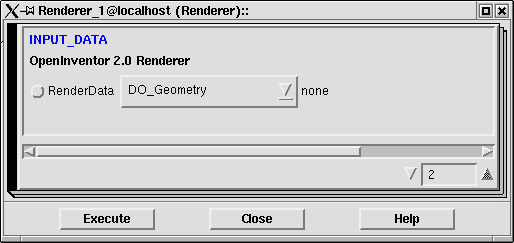
\includegraphics[scale=0.7]{renderer/pict/image2}
   \caption{Renderer Module Setup in the MapEditor}
	\label{fig49}
  \end{center}
 \end{figure}
 \endlatexonly

 

\section{Cooperative Working Modes}

see Chapter 5, COVISE CE, section MasterCtrl, subsection Synchronization

%The COVISE renderer is able to communicate with other renderers in a cooperative
%working session in a master/slave relationship. The communication between
%renderers is done by passing special kinds of messages via the controller.
%That means, no renderer knows anything about the existence of any other renderer.
%For the user the updating of the scene view in the cooperative environment is
%handled transparently. As already mentioned, there is a master/slave relationship
%established in a cooperative session. If the master e.g. translates the camera
%view by dragging the mouse, the view becomes updated on the remote renderer's side. 

%Currently in tight coupled and master/slave relationship the 

%\begin{itemize}
%\item Telepointer
%\item Object transformations
%\item Camera positions
%\item Draw style and draw mode
%\item Picking/editing mode
%\item Background color editing
%\item Switching of fog, antialiasing and axes on/off
%\end{itemize}

%become automatically updated in the other slave renderer windows. Advanced features
%like changing material properties or adding new lights to a scene are merely thought
%for local use and postprocessing of data and therefore not sent to the partners.
%However, the most important thing for cooperative working, that is the placement,
%the orientation of objects and the viewers perspective in respect to the scene,
%are always the same for all partners.
%(Strictly speaking, there is a
%slight difference between "Master/Slave Mode" and "Tight Coupling": "Master/Slave" causes the slave
%renderer to be updated at the end of a move only, whereas "Tight" makes a contiuous update. The two
%possibilities have been introduced due to performance considerations.)



\subsection{Using the Telepointer}

see Chapter 5, COVISE CE, section MasterCtrl, subsection Telepointer

%In addition to the COVISE multimedia support, the renderer introduces the Telepointer.
%The telepointer operates in all directions. If you press the SHIFT key on your
%keyboard, your machine's name will appear at your current mouse position in the
%other renderer's drawing areas. To set the telepointer to another position,
%release the SHIFT key, move the mouse and press SHIFT again at the new position,
%or move the mouse while the SHIFT key is still pressed.

\section{The Renderer's User Interface}

In the following sections the components of the renderer user interface are discussed.

\html{\htmladdimg{pict/general.png}} 
 \latexonly
 \begin{figure}[htp]
  \begin{center}
   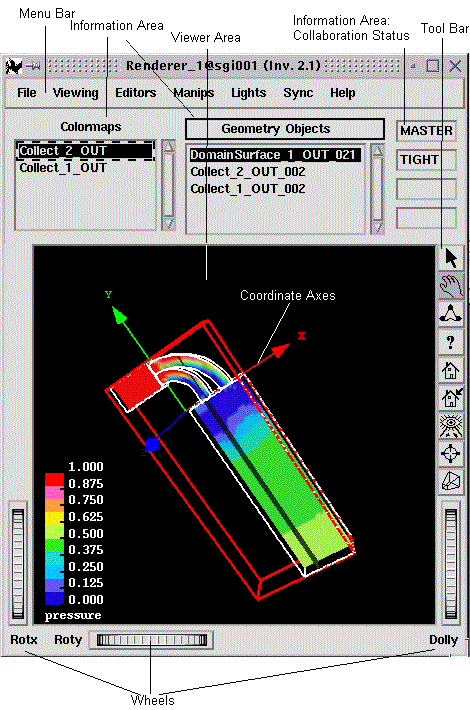
\includegraphics[scale=0.7]{renderer/pict/general}
   \caption{Renderer Main Window Components}
	\label{fig50}
  \end{center}
 \end{figure}
 \endlatexonly

\clearpage

\subsection{The Viewer Area}

In the viewer area objects are displayed and can be manipulated in several ways.
The coordinate axes show the current view orientation.

\subsubsection{Direct Interaction}

Using the mouse buttons in viewing mode affects the camera position, the line of
sight, and the angle of vision in respect to the scene. In the default viewing mode,
the mouse buttons have the functionality as described earlier. In edit (pick)
mode, pressing the left mouse button selects the object under the mouse cursor.
When seeking is enabled by clicking on the seek icon, pressing the left mouse
button starts seeking to the selected point.

% \html{\htmladdimg{pict/image4.png}} 
% \latexonly
% \begin{figure}[htp]
%  \begin{center}
%   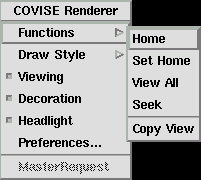
\includegraphics[scale=0.7]{renderer/pict/image4}
%   \caption{The Viewer Popup Menu}
%	\label{fig51}
%  \end{center}
% \end{figure}
% \endlatexonly

 \html{\htmladdimg{pict/popup.png}} 
 \latexonly
 \begin{figure}[htp]
  \begin{center}
   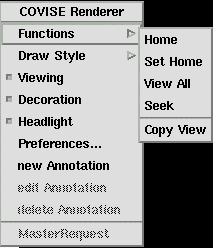
\includegraphics[scale=0.7]{renderer/pict/popup}
   \caption{The Viewer Popup Menu}
	\label{fig51}
  \end{center}
 \end{figure}
 \endlatexonly


\subsubsection{The Viewer Popup Menu}

The popup menu (\ref{fig51}) is activated by clicking the right mouse button while
the mouse pointer is positioned in the viewer area. The popup menu contains
several items and sub menus. These are:

\begin{itemize}
\item {\bf Functions}: The items of this popup sub menu correspond to the icons
on the right side of the viewer area.

\item {\bf Draw Styles}: There are two drawing modes (Still Mode and Move Mode) and seven different drawstyles
for each of these modes, among which the user can choose.   Move Mode is
automatically enabled when interactively moving objects or the camera
using the mouse. The objects may be rendered in a simpler style when
selecting one of the menu items. This is especially useful on slower
machines; thus z-buffering is turned off while rendering in these styles.
The different mode items are:

\begin{itemize}
\item As is
\item Hidden Line
\item No Texture
\item Low Resolution
\item Wireframe
\item Points
\item Bounding box
\end{itemize}

The last three items of the drawstyle sub menu in the viewer popup menu activate
single buffering, double buffering or the switching between single buffering
during manipulation and double buffering otherwise.

% \html{\htmladdimg{pict/image6.png}} 
% \latexonly
% \begin{figure}[htp]
%  \begin{center}
%   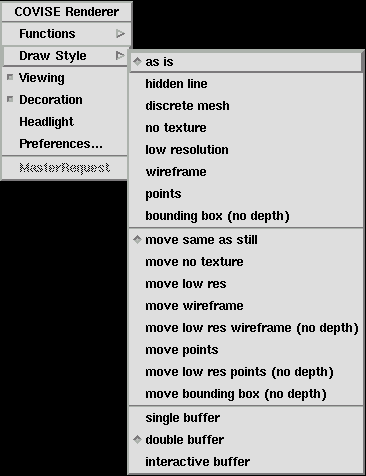
\includegraphics[scale=0.7]{renderer/image6}
%   \caption{Available Drawstyles in the Viewer Popup Menu}
%	\label{fig52}
%  \end{center}
% \end{figure}
% \endlatexonly

 \html{\htmladdimg{pict/drawstyle.png}} 
 \latexonly
 \begin{figure}[htp]
  \begin{center}
   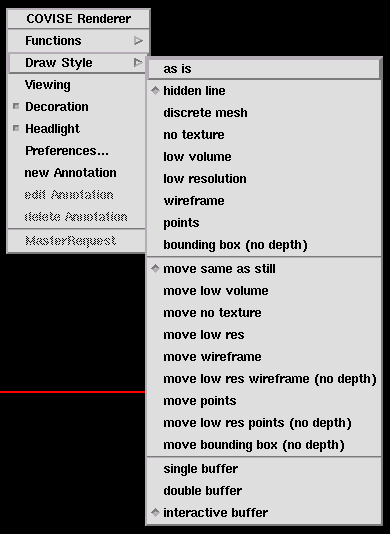
\includegraphics[scale=0.7]{renderer/pict/drawstyle}
   \caption{Available Drawstyles in the Viewer Popup Menu}
	\label{fig52}
  \end{center}
 \end{figure}
 \endlatexonly
 
You can see different viewing modes in  \ref{fig53}, \ref{fig54}, and \ref{fig55}. The
hidden line representation removes all lines which normally could be seen 
shining through in a wireframe representation.

 \html{\htmladdimg{pict/image8.png}} 
 \latexonly
 \begin{figure}[htp]
  \begin{center}
   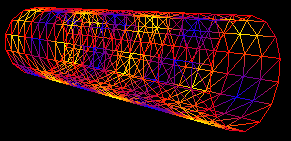
\includegraphics[scale=0.7]{renderer/pict/image8}
   \caption{Wireframe Representation}
	\label{fig53}
  \end{center}
 \end{figure}
 \endlatexonly

 \html{\htmladdimg{pict/image9.png}} 
 \latexonly
 \begin{figure}[htp]
  \begin{center}
   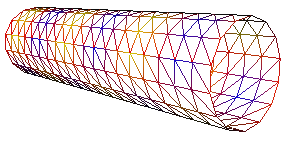
\includegraphics[scale=0.7]{renderer/pict/image9}
   \caption{Hidden Line Representation}
	\label{fig54}
  \end{center}
 \end{figure}
 \endlatexonly

 \html{\htmladdimg{pict/image10.png}} 
 \latexonly
 \begin{figure}[htp]
  \begin{center}
   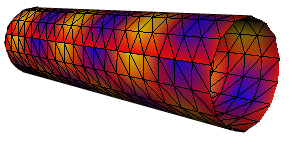
\includegraphics[scale=0.7]{renderer/pict/image10}
   \caption{Discrete Representation}
	\label{fig55}
  \end{center}
 \end{figure}
 \endlatexonly

\clearpage

\item {\bf Viewing}: Toggles between View and Edit (Pick) mode. When picked, a red bounding
box appears surrounding the selected object (\ref{fig56}). 

 \html{\htmladdimg{pict/image11.png}} 
 \latexonly
 \begin{figure}[htp]
  \begin{center}
   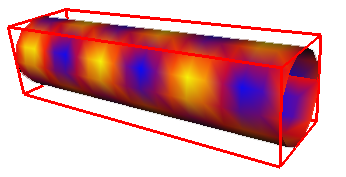
\includegraphics[scale=0.7]{renderer/pict/image11}
   \caption{A Selected (Picked) Object}
	\label{fig56}
  \end{center}
 \end{figure}
 \endlatexonly

When you click on the background in the viewer area the object becomes deselected
again. You can only select one object at a time.

\item {\bf Decoration}: Hides and shows the decoration around the render area. The render area appears a
bit enlarged while decoration is hidden.

\item {\bf Headlight}: Switches the headlight on and off. If you are in PHONG shading mode and no other
lights are active, the objects may become invisible depending on the direction of
the normals on the object surface. It is possible to add more lights to a scene.
This is described later in this chapter.

\item {\bf Preferences}: You can select options from the Preference Sheet:
 \html{\htmladdimg{pict/image12.png}} 
 \latexonly
 \begin{figure}[htp]
  \begin{center}
   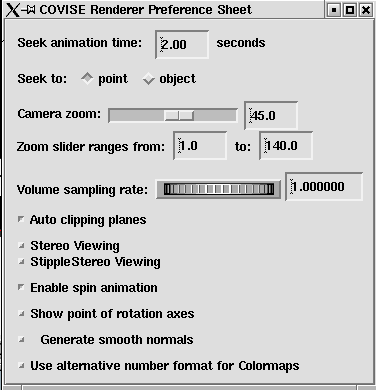
\includegraphics[scale=0.7]{renderer/pict/image12}
   \caption{The Preference Sheet}
	\label{fig57}
  \end{center}
 \end{figure}
 \endlatexonly
\clearpage
 
A menu appears in which defaults for the seek mode, zoom slider bounds, clipping
planes and stereo viewing can be set, or an {\bf alternative number format for colormaps} can
be specified:\newline
This field can be used to specify formats of the numbers along the
color legend. It must be a float format for the "printf" format as
specified in the unix manual pages and should be left-justified.
\begin{verbatim}
Examples: Values 0 0.1 0.2 0.3 0.4 0.5

Format: %-.3f   -->   0.000 0.100 0.200 0.300 0.400 0.500
        %-.2f   -->   0.00 0.10 0.20 0.30 0.40 0.50
\end{verbatim}	
The Volume sample rate thumbwheel is needed for
Volume Rendering (see Appendix).

%When stereo viewing is enabled, a thumb wheel appears, where the stereo offset
%can be adjusted to improve the stereo impression (See "Stereo Viewing Mode" on
%page 58). 

When Spin Animation is enabled, objects can be rotated around in an
animated fashion in viewer mode.


\item {\bf Annotation} (new, edit, delete): With the items of this sub menu (new Annotation / edit Annotation /
delete Annotation) you can add a description to the Renderer image, like "isosurface" in
the figure below.

 \html{\htmladdimg{pict/annotation.png}} 
 \latexonly
 \begin{figure}[htp]
  \begin{center}
   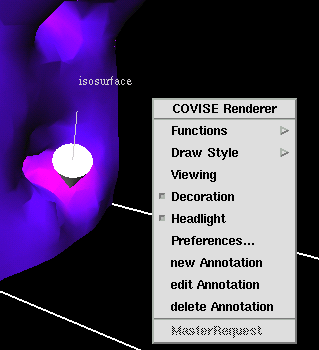
\includegraphics[scale=0.7]{renderer/pict/annotation}
   \caption{Annotion function}
	\label{fig57a}
  \end{center}
 \end{figure}
 \endlatexonly
 
Switch to pick mode and click on the detail you want to explain:
You can now (using a popup with "apply")
\begin{itemize}
\item add a {\bf new Annotation}
\item {\bf edit} an existing {\bf Annotation}
\item {\bf delete} an {\bf Annotation}
\end{itemize}

Please note:
\begin{itemize}
\item Annotations can be saved as part of a map
\item Annotations are "static" - they do not move e.g. with an isosurface if the isovalue is changed
\end{itemize}

\item {\bf MasterRequest}: same function as MasterCtrl in MapEditor

\end{itemize}
\clearpage

\subsubsection{The Decoration Area}

The decoration consists of three thumb wheels for rotating (Rotx, Roty) and
zooming (Dolly) as well as a zoom slider trim (Zoom) and six viewer icons to
the right side of the viewer area. These icons are shortcuts for some of the
viewer pop-up functionality. From top to bottom there are icons for 

\begin{itemize}
\item switching between View and 
\item Edit (Pick) Mode
\item Head Tracking Mode (currently not implemented)
\item invoking the help browser (Help) - not implemented, use help button in menu bar instead
\item resetting camera position to the home position (Home)
\item saving a new home position for the camera view (Set Home)
\item viewing the whole scene (View All)
\item seeking to a certain point of the scene (Seek)
\end{itemize}

\clearpage

\subsection{The Menu Bar}

The menu bar of the renderer window is shown below.

 \html{\htmladdimg{pict/menubar.png}} 
 \latexonly
 \begin{figure}[htp]
  \begin{center}
   
\includegraphics[scale=0.7]{renderer/pict/menubar}
   \caption{Renderer Menubar}
	\label{fig58}
  \end{center}
 \end{figure}
 \endlatexonly

\subsubsection{File Menu}

 \html{\htmladdimg{pict/image13.png}} 
 \latexonly
 \begin{figure}[htp]
  \begin{center}
   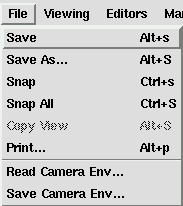
\includegraphics[scale=0.7]{renderer/pict/image13}
   \caption{The File Menu}
	\label{fig59}
  \end{center}
 \end{figure}
 \endlatexonly

\begin{itemize}
\item {\bf Save}: The current objects are saved in Inventor 3D format. Programs reading this format
like IRIS Explorer or IRIS Showcase can load this objects and allow further usage
and postprocessing of the 3D data.

\item {\bf Save as}: Save the whole scene. A file selector box appears where directory and file name
can be selected.

\item {\bf Snap}: Take a snapshot of the viewer area. Format of the snapshot files is .tiff
(changed with Rel. 5.2.3). Creates an error dialog if offscreen rendering
is not possible due to low colordepth. Offscreen rendering requires at
least a 24bit true color. Same applies to Snap all.

\item {\bf Snap all}: Take a series of snapshots of the viewer area.\newline
You can use this series of snapshots in order to {\bf generate a simple
movie}.\newline
Example on SGI: call {\bf 'mediaconvert'} and fill in the entries as shon below

\html{\htmladdimgpict{pict/mediaconvert.png}} 
 \latexonly
 \begin{figure}[htp]
  \begin{center}
   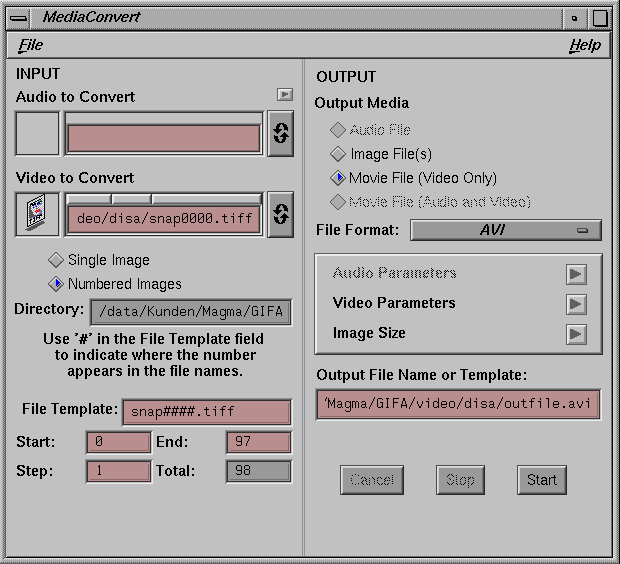
\includegraphics[scale=0.6]{renderer/pict/mediaconvert}
   \caption{MediaConvert - Movie on SGI}
	\label{fig59a}
  \end{center}
 \end{figure}
 \endlatexonly
\clearpage

\item {\bf Copy View}: The currently selected object is copied to a buffer from which other programs
like IRIS Showcase can directly paste the 3D object into their application. 

\item {\bf Print}: It is possible to save the currently visible scene in an Postscript file or to
send the postscript output directly to a printer. The available printers are
listed below in the printer list. The output quality and print size in inches
can be adjusted The page format can be chosen between landscape or portrait.

 \html{\htmladdimg{pict/image14.png}} 
 \latexonly
 \begin{figure}[htp]
  \begin{center}
   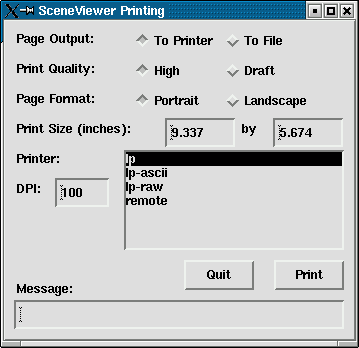
\includegraphics[scale=0.7]{renderer/pict/image14}
   \caption{The Printing Menu}
	\label{fig60}
  \end{center}
 \end{figure}
 \endlatexonly

\item{\bf Read/Save Camera Env...}: Restore/Save the camera environment

\end{itemize}
\clearpage

\subsubsection{Viewing menu}

The viewing menu is shown in \ref{fig61}.

\begin{itemize}
\item {\bf Pick/Edit}:

By default the renderer is in the View mode. The viewer uses a virtual
trackball to rotate the scene graph around the point of interest. If you want
to change the view of a scene but a specific object in respect to other objects,
you have to switch from the View mode to Pick/Edit mode. In Edit mode the
outlined hand cursor changes to an arrow shape cursor. If you click on an object
with the left mouse button, the object becomes selected and highlighted by a
red wireframe box which now surrounds the object. You can select only one object
at a time. If you have opened any editors or enabled manipulators, these will
be attached to the selected target object for further editing. If you switch
between objects by clicking on a different object all manipulators and editors
automatically become attached to this object.

 \html{\htmladdimg{pict/image15.png}} 
 \latexonly
 \begin{figure}[htp]
  \begin{center}
   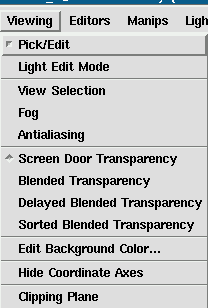
\includegraphics[scale=0.7]{renderer/pict/image15}
   \caption{The Viewing Menu}
	\label{fig61}
  \end{center}
 \end{figure}
 \endlatexonly
\clearpage

\item {\bf Light Edit Mode}:

Enabling this mode lets you interactively edit the current visible light sources
in the scene by using the mouse. 

\item {\bf Fog}:

This item affects the environment of a scene to simulate various atmospheric
effects such as fog, haze, pollution and smoke which are grouped under the term fog.

\item {\bf Anti-aliasing}:

 This technique is useful to eliminate or reduce jagged lines and make objects
 drawn on the screen look smooth. Enabling this item reduces drawing speed.

\item {\bf Screen Door Transparency}:

This and the next three items affect the transparency quality level. Screen
door transparency is the default and the only supported mode on some machines.
For transparency details refer to the editor's section. Screen door
transparency uses GL patterns for achieving the transparency effect.

\item {\bf Blended Transparency}:

 uses GL alpha blending.

\item {\bf Delayed Blended Transparency}:

 uses GL alpha blending, opaque objects are rendered first, then transparent objects.

\item {\bf Sorted Blended Transparency}:

uses GL alpha blending, opaque objects are drawn first, then transparent objects.
Additionally the objects are sorted by their distance from the camera and are
drawn from back to the front.



\item {\bf Edit Background Color}:

Invokes a color editor for changing the background color of the render area (default is black).

\item {\bf Hide Coordinate Axes}:

Toggles between hiding and showing the three coordinate axes. The axes are on by default.

\item {\bf Clipping Plane}: Cut Geometry

\end{itemize}
\clearpage

\subsubsection{Editors menu}

 \html{\htmladdimg{pict/editors.png}} 
 \latexonly
 \begin{figure}[htp]
  \begin{center}
   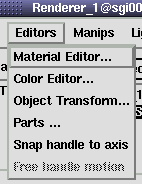
\includegraphics[scale=0.7]{renderer/pict/editors}
   \caption{Editors Menu}
	\label{fig62}
  \end{center}
 \end{figure}
 \endlatexonly

\begin{itemize}
\item {\bf Material Editor}:

The material editor is used for customizing objects by interactively changing
values for ambient, diffuse, specular, transparent, emissive and shininess
elements and immediately seeing the effects of these changes.

 \html{\htmladdimg{pict/image16.png}} 
 \latexonly
 \begin{figure}[htp]
  \begin{center}
   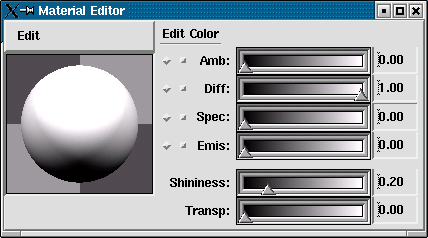
\includegraphics[scale=0.7]{renderer/pict/image16}
   \caption{The Material Editor}
	\label{fig63}
  \end{center}
 \end{figure}
 \endlatexonly



The diffuse color is the object's base color specified in the color array of
the renderer geometry input data objects. If no colors are specified, the color
of each vertex of the object is set to RGB [1.0 1.0 1.0] default. Editing the
diffuse color of those objects affects all vertices of the object, thus the
whole object changes its color. If one color is specified for the whole object
(color binding OVERALL) all vertices of the object are colored according to
this value. If you edit the diffuse color of these objects, also all vertices
are affected by color changes. If vertex based objects such as polygons or
lines with colors attached per vertex (color binding PER\_VERTEX) or per face
(binding PER\_FACE) are present, only the first vertex is affected by changes
of the diffuse color field, therefore editing the diffuse color of those
objects is not very useful. The next items affect the whole object in any
case. The Ambient Color is the reflected color of an object in response to
the ambient lighting in the scene. The default value for this field is [0.2 0.2 0.2].
The Emissive Color is the light caused by self illuminating objects.
The default for this field is [0.0 0.0 0.0], which means the object
is emitting no light. The degree of shininess of an object's surface
is for e.g. achieving metallic effects on the surface of an airplane
wing. The value ranges from 0.0 (default) for a diffuse surface with
no shininess to 1.0 for a highly polished surface. Let us assume there
are two objects present by one object covering the other, where one
cannot see the covered object. By adjusting the Transparency Level of
the covering object you can see either both (values larger than 0.0)
or only the previously covered object (value 1.0).

\item {\bf Color Editor}:

The color editor lets you interactively change the color properties of an
object, a light source or the background color of the render area. You can
set RGB or HSV values or pick a color directly from the color wheel. By
selecting Manual from the edit menu bar item you can prevent changes being
reflected immediately in the object until you are ready. Use the two color
squares to test new colors and store the previous one. By clicking on the
three pads beneath the squares, you can switch back and forth between colors.
The new color is always on the left and the previous color on the right.
You can send the new color to the right square, or the old color to the
left square. RGB values range from 0.0 to 1.0 for the red, green and blue
color component, where [0.0 0.0 0.0] is black and [1.0 1.0 1.0] is white.

 \html{\htmladdimg{pict/image17.png}} 
 \latexonly
 \begin{figure}[htp]
  \begin{center}
   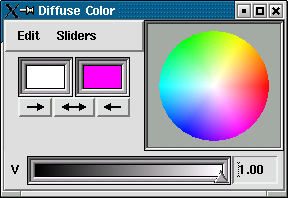
\includegraphics[scale=0.7]{renderer/pict/image17}
   \caption{The Color Editor}
	\label{fig63a}
  \end{center}
 \end{figure}
 \endlatexonly

\item {\bf Object Transform}:

Transform sliders are useful to change the position of objects in respect
to each other or to scale an object to make it appear larger or smaller on
the screen. If you click on an item in the transform slider set sub menus
appear in which you can do the desired editing operations by adjusting
sliders with the mouse or typing exact values using input fields. There
are three different widget layout styles available, simply click on Style
in the slider menu. Note that the changes only affect the currently
selected object in the scene. Translation changes the position of an
object in the scene. Scale changes the size of an object. Rotation
changes the orientation of the object in the scene. Scale Orientation
changes the orientation for scale operations. Center changes the center
around which rotations take place.

 \html{\htmladdimg{pict/image18.png}} 
 \latexonly
 \begin{figure}[htp]
  \begin{center}
   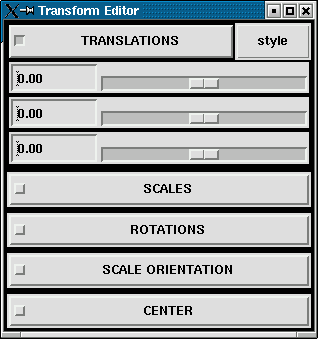
\includegraphics[scale=0.7]{renderer/pict/image18}              
   \caption{The Transform Editor}
	\label{fig64}
  \end{center}
 \end{figure}
 \endlatexonly

\clearpage

\item {\bf Part Editor}:

If the geometry objects displayed by the Renderer can be identified (in case of modules 
using finite elements) you can use the {\bf COVISE Part Editor} to select which parts of 
the geometry will become visible or invisible and, optionally, which part is fixed 
during movements.

 \html{\htmladdimg{pict/partedit.png}} 
 \latexonly
 \begin{figure}[htp]
  \begin{center}
   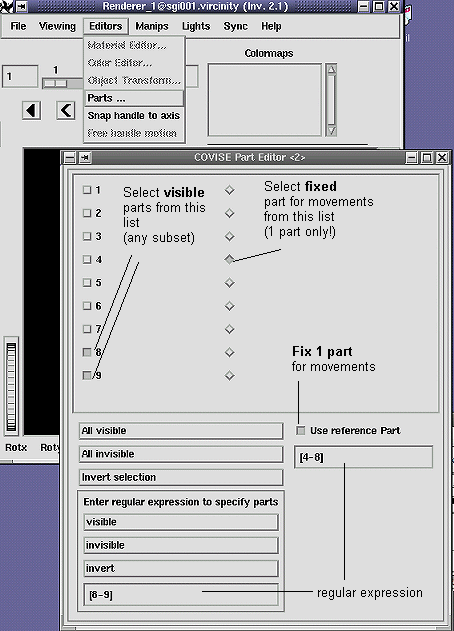
\includegraphics[scale=0.7]{renderer/pict/partedit}
   \caption{Part Editor}
	\label{fig65}
  \end{center}
 \end{figure}
 \endlatexonly

The {\bf left side} of the Part Editor window provides the functions to select which parts 
are {\bf visible}; you have 3 possibilities:
\begin{itemize}
\item Select any subset of parts out of the selection list (toggle switches,any subset)
\item Set all parts visible/invisible or invert your selection
\item Specify the subset of parts by a regular expression and press RETURN
\end{itemize}

On the {\bf right side} you can (optionally) select a {\bf reference part} that will be 
{\bf fixed } during movements; to specify this reference part you can use 2 possibilities:
\begin{itemize}
\item Select this part from the list (toggle switches, 1 part only)
\item Specify a regular expression and press RETURN; the first part matching the 
regular expression is fixed.
\end{itemize}

\clearpage

\item{\bf Interactors (Snap/Free handle)}:

The last two options of the Editors menu item have been added to select options for an 
{\bf Interactor}. If you want to move e.g. a Cutting Surface,
you can attach an interactor to it. An interactor attached to a point of
a Cutting Surface consists of

\begin{itemize}
\item a {\bf tangential plane} (reduced to a square) at that point
\item a {\bf normal} at that point
\end{itemize}
(see example below)

\html{\htmladdimg{pict/interactor.png}} 
 \latexonly
 \begin{figure}[htp]
  \begin{center}
   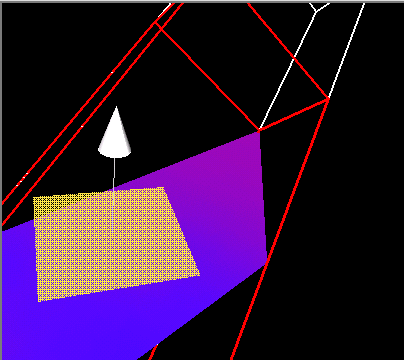
\includegraphics[scale=0.7]{renderer/pict/interactor}
   \caption{Interactor}
	\label{fig65a}
  \end{center}
 \end{figure}
 \endlatexonly
 
You attach an interactor by clicking on a point of the Cutting Surface.

Note: You must be in pick mode and select (click on) the Cutting Surface before you 
can attach an interactor

You can
\begin{itemize}
\item {\bf rotate} the Cutting Surface by using the normal (arrow) as a handle 
\item {\bf translate} the Cutting Surface by pulling the plane
\end{itemize}

You use the option
\begin{itemize}
\item {\bf Snap handle to axis} in order to in order to enable ... 
\item {\bf Free handle motion} in order to disable the orientation of 
CuttingSurfaces normal to coordinate axis
\end{itemize}

\end{itemize}
\clearpage

\subsubsection{Manips menu}

Manipulators are used for direct manipulation of a certain object, like
the editors explained in the last section. 

 \html{\htmladdimg{pict/image19.png}} 
 \latexonly
 \begin{figure}[htp]
  \begin{center}
   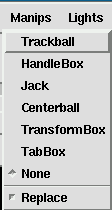
\includegraphics[scale=0.7]{renderer/pict/image19}
   \caption{The Manips Menu}
	\label{fig66}
  \end{center}
 \end{figure}
 \endlatexonly

This way of manipulation is more direct than using editors, but less precise
than using the sliders. To attach a manipulator to an object, switch to the
picking mode and select a manipulator type in the Manips Menu  shown in \ref{fig66}.

Now click on the desired object. The manipulator appears and surrounds
the object. There are different manipulators to transform, rotate, scale,
and move an object in the viewer. 

\begin{itemize}
\item {\bf Trackball}:

This manipulator is for rotating and scaling an object. It appears as a
transparent sphere around the selected object.

 \html{\htmladdimg{pict/image20.png}} 
 \latexonly
 \begin{figure}[htp]
  \begin{center}
   \includegraphics[scale=0.7]{renderer/pict/image20}
   \caption{Object with Trackball Manipulator Attached}
	\label{fig67}
  \end{center}
 \end{figure}
 \endlatexonly
\item {\bf Handle Box}: This inserts a transparent cube into the scene that allows the user to
scale and translate the object by moving the mouse in various ways.
Use the SHIFT and ALT keys with the left mouse button to achieve specific
effects for both the trackball and the handlebox manipulator. (see \ref{fig68})

\item {\bf Jack}: The object can be zoomed and rotated.

\item {\bf Centerball}: Is for moving the center point of rotation for an object. Afterwards
the object can be rotated around the new rotation point.

\item {\bf TransformBox}: This manipulator is for transforming the selected object. 

\item {\bf TabBox}: This lets you scale an object by doing a click-drag-release motion with
the mouse after clicking on the green control points.

\item {\bf None}: This is the default. If an object gets picked, no manipulator is attached to the object.

\item {\bf Replace}: If a different manipulator is selected from the list the currently active
manipulator is either replaced or stays attached. 

 \html{\htmladdimg{pict/image21.png}} 
 \latexonly
 \begin{figure}[htp]
  \begin{center}
   \includegraphics[scale=0.7]{renderer/pict/image21}
   \caption{Tube Surrounded by a Handlebox Manipulator}
	\label{fig68}
  \end{center}
 \end{figure}
 \endlatexonly
\end{itemize}

\clearpage


\subsubsection{Lights menu}

The lights menu is for creating, editing, and removing light sources
in an object scene. This is a feature used for changing the appearance
of an object by changing its illumination. Light information is
currently not sent to other renderers in a cooperative working environment.
Each entry in the menu is explained now in detail.

 \html{\htmladdimg{pict/image22.png}} 
 \latexonly
 \begin{figure}[htp]
  \begin{center}
   \includegraphics[scale=0.7]{renderer/pict/image22}
   \caption{The Lights Menu}
	\label{fig69}
  \end{center}
 \end{figure}
 \endlatexonly

\begin{itemize}
\item {\bf Lightmodel BASE\_COLOR}: Each object has its own base color also called diffuse color. If no
colors are specified, the objects are colored white over all faces
or vertices. When the base color model is enabled (the default), all
objects are rendered by taking only their diffuse color into account.
If it is disabled all objects are PHONG shaded. The PHONG lighting
model takes into account all light sources in the scene and the object's
surface orientation (the normals on faces or vertices) with respect to
the lights to generate a realistic smooth shaded 3D appearance of an
object. Scientists often prefer to see only the real colors defined
for the object without shading effects, so switching between the two
modes is introduced here.
\item {\bf Create Dir Light}: This creates a light which illuminates uniformly along a particular direction.

\item {\bf Create Point Light}: A point light, like a star, radiates light equally in all directions
from a given location in 3D space.

\item {\bf Create Spot Light}: A spot light illuminates from a point in space along a primary direction.
Its illumination is a cone of light diverging from the light's position.
This feature is hardware dependent. If not supported, a spotlight appears
as a point light.

 \html{\htmladdimg{pict/image23.png}} 
 \latexonly
 \begin{figure}[htp]
  \begin{center}
   \includegraphics[scale=0.7]{renderer/pict/image23}
   \caption{The Spot Light Icon}
	\label{fig69}
  \end{center}
 \end{figure}
 \endlatexonly

\item {\bf Ambient Lighting}: This is used for the PHONG lighting mode, it lets you edit the ambient
ligthing in the scene.

\item {\bf Turn all ON}: Turns all currently defined light sources on.

\item {\bf Turn all OFF}: Turns all currently defined light sources off.

\item {\bf Show all Icons}: Shows the icons of the currently defined light sources.

\item {\bf Hide all Icons}: Hides the icons of the currently defined light sources.

\item {\bf Headlight}: This is the default light. A sub menu lets you edit the color of this
light or removing it from the scene. The icon for the headlight is turned off by default. If you create new lights, new entries will appear below. 

\item {\bf New lights}: are shown by placing the light icon at a default position in the scene.
These lights can be edited interactively with the mouse after turning
on the Light editing mode. To edit the properties of a light you can
also select Edit from the sub menu of the Headlight item.
The edit window appears, displaying the light you have selected.
You can change the intensity of the light emanating from the source
by moving the intensity slider. You can also adjust the angle at which
the light shines on the object by clicking on the directional arrow and
changing its position in the window. Editing the color of the light
brings up the color editor. 

 \html{\htmladdimg{pict/image24.png}} 
 \latexonly
 \begin{figure}[htp]
  \begin{center}
   \includegraphics[scale=0.7]{renderer/pict/image24}
   \caption{New Light Entries}
	\label{fig70}
  \end{center}
 \end{figure}
 \endlatexonly
 
 \html{\htmladdimg{pict/image25.png}} 
 \latexonly
 \begin{figure}[htp]
  \begin{center}
   \includegraphics[scale=0.7]{renderer/pict/image25}
   \caption{The Light Editor Menu}
	\label{fig71}
  \end{center}
 \end{figure}
 \endlatexonly

\end{itemize}
\clearpage

\subsubsection{Sync menu}

\html{\htmladdimg{pict/image26.png}} 
 \latexonly
 \begin{figure}[htp]
  \begin{center}
   \includegraphics[scale=0.7]{renderer/pict/image26}
   \caption{The Sync Menu}
	\label{fig72}
  \end{center}
 \end{figure}
 \endlatexonly
 
see Chapter 5, COVISE CE, section MasterCtrl, subsection Synchronization

%relationship has been established between the partners of a working session.
%From the renderer's point of view this means that there is only one
%partner who has all of the interaction facilities. This is often
%inconvenient. Assume other partners want to save a certain scene or
%object without having to ask the master to take over control for this
%single operation.

%COVISE offers three degrees of coupling:

%\begin{description}
%\item[Loose Coupling] mode has been introduced as an addition to the master/slave and tight
%coupling mode.
%If the master enables this mode all partners have the same interaction
%facilities as the master. Camera positions and object transformations
%are no longer sent to other renderers. Only the master has the ability
%to switch between the two modes. If the mode is set back to master/slave
%all manipulators and editors become detached and invisible and the menu
%bar is set to insensitive in the slave renderers. Additionally, the
%scene is updated according to the view in the master renderer.  
%\item[Master/Slave] Slave Renderers controlled by Master - update at the end of a move 
%operation. This is the {\bf default} cooperative mode.
%\item[Tight Coupling] Slave Renderers controlled by Master - continuous update. 

% \html{\htmladdimg{pict/image26.png}} 
% \latexonly
% \begin{figure}[htp]
%  \begin{center}
%   \includegraphics[scale=0.7]{renderer/pict/image26}
%   \caption{The Sync Menu}
%	\label{fig72}
%  \end{center}
% \end{figure}
% \endlatexonly

%\end{description}

\subsubsection{Help}

Pressing Help provides you online help for the Renderer - but you can easily branch e.g. to help for
MapEditor or Modules. 

\clearpage

\subsection{The Information Area}

 \html{\htmladdimg{pict/general.png}} 
 \latexonly
 \begin{figure}[htp]
  \begin{center}
   \includegraphics[scale=0.7]{renderer/pict/general}
   \caption{Information Area of the Renderer}
	\label{fig73}
  \end{center}
 \end{figure}
 \endlatexonly

On the left side of the information area, the list of currently displayed geometry objects is shown
(together with the colormaps used).

 \html{\htmladdimg{pict/image28.png}} 
 \latexonly
 \begin{figure}[htp]
  \begin{center}
   \includegraphics[scale=0.7]{renderer/pict/image28}
   \caption{List of Current Geometry Objects and Color Maps}
	\label{fig74}
  \end{center}
 \end{figure}
 \endlatexonly
 
If you click on a certain object in the render area the name of the object gets highlighted in the object list. It is also possible to select an object in the render area by clicking on it's name in the object list. The red bounding box appears around the selected object in the render area to highlight the selection.
Thus, similar objects can be distinguished by their unique name.


On the right side of the information area there are four lines; the first two display the
collaboration status of the renderer:

\begin{itemize}
\item {\bf Interaction Mode}: Shows whether the renderer is master or slave.

\item {\bf Synchronization}: Tells whether tight, master/slave (=SYNC), or loose coupling is enabled between the renderers in the environment.

\item {\bf Rendering State}: - obsolete, not used

\item {\bf Rendering Time}: - obsolete, not used

\end{itemize}


\section{Using Spaceball and Spacemouse}

% commented following image - logitec no longer present in updated version

% \html{\htmladdimg{pict/image12.png}} 
% \latexonly
% \begin{figure}[htp]
%  \begin{center}
%   \includegraphics[scale=0.7]{renderer/pict/image12}
%   \caption{CrystalEyes Shutter Glasses, Logitech Ultra Sonic Transmitter and Spacemouse}
%	\label{fig575}
%  \end{center}
% \end{figure}
% \endlatexonly

If the Spaceball or the DLR Spacemouse is connected to your workstation, you are able to manipulate the geometry objects in 3D space in a six degrees of freedom fashion. The device should beep two times at renderer startup time when initialization of the device was successful. To move an object around select the object in picking mode. The device is now attached to the selected object. Some of the device buttons provide some additional functionality:

\begin{itemize}
\item Button 1: Disable/enable rotation
\item Button 2: Disable/enable translation
\item Button *: Set home selected object
\item Button 3: Set home all objects
\end{itemize}

If no object is selected, the spacemouse changes the viewpoint in respect
to the scene by changing the current camera position. 

\section{Stereo Viewing Mode}


 \html{\htmladdimg{pict/image29.png}} 
 \latexonly
 \begin{figure}[htp]
  \begin{center}
   \includegraphics[scale=0.7]{renderer/pict/image29}
   \caption{Stereo mode in the preference sheet}
	\label{fig76}
  \end{center}
 \end{figure}
 \endlatexonly
Some platforms support stereo in a window viewing. Stereo viewing is enabled
by choosing Stereo Viewing in the renderer's preference sheet. You return to
the default mode by deselecting Stereo Viewing in the preference sheet or
typing in a shell window: 

/usr/gfx/setmon -n 72HZ
or
/usr/gfx/setmon -n 60HZ
depending on the type of monitor attached. 

\section{Head Tracking Mode}

currently not implemented

%When a Logitech Head Tracking Device with CrystalEyes shutter glasses is
%connected to a serial port, the visualized data  can be investigated by
%moving  your head. By turning the head, objects can be seen from a different
%angle and by moving the head forward or backward, objects can be seen closer
%or farther. Thus, it is possible to see object from different sides or "fly"
%through a data set. In conjunction with stereo viewing  a much more immersive
%impression is provided to the user which can be helpful in many 3D scientific
%visualization cases. The serial port can be adjusted in the preferences menu.
%It is also possible to use a Polhemus Fastrak tracking device for position
%and orientation detection.

%\section{Performance Considerations in a Cooperative Session}

%Particularly for performance reasons, it is advantageous to know little
%about what is going on behind the scenes when the mouse is moved around
%in the viewer area, especially when working with the master renderer in
%the environment.

%\subsection{Updating the Telepointer}

%The telepointer is operating in all directions. If you press the SHIFT
%key on your keyboard, your machine's name will appear at your current
%mouse position in the other renderer's drawing areas. To reposition the
%telepointer to another position, release the SHIFT key, move the mouse
%and press SHIFT again at the new position, or move the mouse while the
%SHIFT key is still pressed. The difference here is, that in the second
%case the new mouse position is sent over the network very often.

%\subsection{Updating the Head Tracker}

%In head tracking mode, the current tracking update rate can be adjusted
%by the thumbwheel in the viewer preference sheet. A lower update rate
%produces less network traffic. The default tracking rate is currently
%0.1sec. The ideal tracking rate depends heavily on the scene complexity
%and hardware platform used. Also note that the others partner's graphics
%hardware might be not able to render at your locally available graphics
%speed. If you want the head tracking to have only local effect, change
%to loose coupling in the sync menu of the renderer's menu bar. When you
%switch back to tight coupling later on, the screens become automatically
%updated and synchronized again.






    
%\subsubsection{Direct Manipulation}

%Normally, new positional information is only sent, when the master
%releases the mouse button in the viewer area. 

%\subsubsection{Using the Decoration Around the Viewer Area}

%The same is true for the thumb wheels and the slider around the
%viewer. When you release the mouse button information is sent over
%the network. 

%\subsubsection{Using Sliders}

%As far as the sliders in the transform editor are concerned, the situation
%is somewhat different. If you are using the transform sliders by pressing
%the mouse button and moving back and forth, every little movement will
%directly go over the network. If you want to avoid this, click on the
%slider once at the desired position or use the input line. Note that
%renderers running on machines without advanced graphics hardware can
%manually change the scene drawstyle changed to wireframe or points for
%locally doing extensive editing operations. This especially applies to
%the master/slave mode.

%\subsection{System Requirements}

%The COVISE renderer is based on the OpenInventor high level object oriented 
%graphics toolkit developed by Silicon Graphics. OpenInventor itself uses 
%OpenGL, the 3D graphics standard as its rendering interface.

%SGI Systems ship with OpenInventor 2.1 and OpenGL 1.2, there are no
%additional requirements.

%The Rendering speed can vary significantly, depending on the graphics
%adaptor and the quality of the OpenGL implementation. Currently we support SGI, HP and Linux platforms.
%Spacemouse/Spaceball as input device is currently only supported in the SGI
%version.


%Another thing regarding OpenInventor has to be mentioned: On SGI we currently
%support three different Inventor releases: 1.1, 2.0 and 2.1.2. Depending on
%the eoe subsystem installed on your machine there should exist a link from
%one of these renderers (Renderer11,Renderer20,Renderer21) to a module called renderer. 

			% using the Desktop Renderer (Uwe Woessner)

\begin{htmlonly}


\usepackage{html, htmllist}
\usepackage{longtable}

\bodytext{bgcolor="#ffffff" link="#0033cc" vlink="#0033cc"}

%%%==================================================	
%%%==================================================	

% #1  mark defined by \label
% #2  a linktext 
% #3  a html link 
\newcommand{covlink}[3]{\htmladdnormallink{#2}{#3} \latex{(\ref{#1})} }


\newenvironment{covimg}[4]%
{
 \begin{figure}[htp]
  \begin{center}
   \latexonly
      \includegraphics[scale=#4]{#1/pict/#2}
   \endlatexonly  
   \html{\htmladdimg[align="center"]{pict/#2.png}}
   \caption{#3}
  \end{center}
 \end{figure} 
}{} 

\newenvironment{covimg2}[3]%
{ 
 \begin{figure}[htp]
  \begin{center}
     \latexonly
       \includegraphics[scale=#3]{#1/pict/#2}   
     \endlatexonly
     \html{\htmladdimg[align="center"]{pict/#2.png}}
  \end{center}
 \end{figure} 
}{}

\definecolor{output}{rgb}{0.,0.,1.}
\definecolor{depend}{rgb}{1.,0.65,0.}
\definecolor{required}{rgb}{0.58,0.,0.83}
\definecolor{optional}{rgb}{0.,0.39,0.}

\newcommand{\addimage}[1] {\html{\htmladdimg{pict/#1.png}}}

\newcommand{\addpict}[4] {\latexonly
	     \begin{figure}[!htbp]
			  \begin{center}
   	 		  \includegraphics[scale=#1]{#2}
   	 		  \caption{#3}
		 		  \label{#4}
			  \end{center}
	 		\end{figure}
	     \endlatexonly}



\newcommand{\mapeditor}{\textbf{Map Editor}}
\newcommand{\covise}{\textbf{COVISE}}


\end{htmlonly}


%=============================================================
\startdocument
\chapter{COVISE CE (Collaborative Engineering)}
\label{CollabEngineering}
%=============================================================

\section{Architecture and Configuration}
\label{Architecture}

\subsection{Architecture Summary}
\label{Architecture_Summary }

%{\bf Note:}

{\bf Usage Hints:}
\vspace{0.5cm}

This short introduction has been prepared for users with basic experience in using
COVISE VR in a standalone environment only; for this user group it provides the necessary
background to extend the use of COVISE to Collaborative Engineering, i.e. COVISE CE. The information 
has been collected from the Tutorial, the first chapters of the (old) User's Guide, and other sources
to provide one reference chapter for these users. 
   
\vspace{0.5cm}

For collaborative working you can either use COVISE CE alone - as described in this document - or
you can extend a collaborative COVISE session to a complete (virtual) meeting, using  
{\bf \begin{htmlonly}N'S³\end{htmlonly}\latexonly N'S$^3$\endlatexonly (COVISE Conference
Room Interface)}.
The Conference Room Interface (optional feature, described in a separate document)
\begin{itemize}
\item has been developed in the framework of the \begin{htmlonly}N'S³\end{htmlonly} 
\latexonly N'S$^3$\endlatexonly (ENScube) project.
\item is based on Sametime (Sametime is a trademark of IBM Lotus Corporation)
\end{itemize} 
\vspace{0.5cm}

{\bf Architectural Concepts:}

For collaborative working with COVISE you should know the basic architectural concepts of COVISE.
After having read this chapter you will be familiar with:

\begin{itemize}
\item The Architecture of COVISE
\item how to prepare COVISE for a distributed or collaborative session
\end{itemize}

In COVISE it is possible to run modules on remote computers. This is also known as 
"Distributed Computing". By distributing modules across a network one can make use 
of remote resources for example of a compute server with more CPUs or memory than on a 
local workstation or PC. The COVISE session is controlled from the Mapeditor on the
local workstation. Remote hosts are included in the session via the menu item 
CSCW \latexonly $>>$ \endlatexonly \begin{htmlonly} > > \end{htmlonly} AddHost (CSCW = \underline{C}omputer
\underline{S}upported \underline{C}ollaborative \underline{W}ork).

In a multiuser session each participant has his own Mapeditor and Renderer. The 
session has to be initiated by one partner who adds the other partners to the 
session (menu item CSCW \latexonly $>>$ \endlatexonly \begin{htmlonly}> > \end{htmlonly} AddPartner). The initiating partner plays the master role, 
which means that he has the control over the Mapeditor and the Renderer. If he e.g. 
changes the camera position in the Renderer all other partner's cameras are synchronised 
with the master camera. The master role can be exchanged between partners. This way of 
working together in a multiuser session is also known as "Collaborative Working" or - for COVISE
applications - as "Collaborative Engineering" where COVISE is regarded as a "Shared Application" 
which is aware of the sharing.

As the hosts of the partners can also be used for distributed computing COVISE extends 
far beyond a "Shared Application" such as the ones based on X Windows sharing or a 
Windows application shared via Netmeeting.

The next sections provide background information on the COVISE architecture and explain how a 
distributed session (Distributed Computing) or a collaborative 
session (for Collaborative Engineering) is implemented.

\begin{longtable}{|p{14cm}|}
\hline
\newline
{\bf See also: Additional feature COVISE daemon "covised":}\newline
The COVISE daemon "covised" - included as a {\bf preversion} in Rel. 5.2 - 
provides a more general and more comfortable user interface for collaborative 
working than CSCW, using a concept of "rooms" (working groups - can be {\bf predefined}) 
like N'S³ (see {\bf 5.6 New Collaborative COVISE})\newline 
\\									
\hline
\end{longtable}


\subsection{Distributed Computing}
\label{distributed}

In {\bf COVISE} it is possible to run modules on remote computers. This is also 
known as {\it Distributed Computing}. By distributing modules across a network 
remote resources are used for example of a compute server with 
more CPUs or memory than o<Zwischenablage leer>n your local workstation or PC. The {\bf COVISE} 
session is controlled from the {\bf MapEditor} on the local workstation. 

	
\begin{covimg}{collab}{distr-a}{Distributed Session (Distributed
Computing)}{0.5}\end{covimg}
\begin{htmlonly}
Figure 5.1: Distributed Session (Distributed Computing)
\vspace{0.5cm}
\end{htmlonly} 
  
The previous figure shows the elements of an example for 
distributed working in {\bf COVISE}. The 
application consists of three modules: a module which reads in data (READ) 
a module which extracts a special feature (FILTER) and a module which displays 
the extracted data (RENDER). As the filter module consumes much CPU 
time and memory it will be started on a remote compute server, also the Reader because the data  
to be read in is on the remote machine. 
The first process started by {\bf COVISE} is the {\bf Controller} 
which in turn starts the user interface process {\bf MapEditor} and the data 
management process {\bf CRB}. As soon as another host is included in the 
session a {\bf CRB} is started on that computer. The read module is started on the 
local workstation, the filter module on the remote computer  and the 
renderer on the local workstation. The green arrows between the processes 
{\bf Controller}, {\bf MapEditor}, {\bf CRB} and the modules indicate TCP sockets, the blue arrows 
indicate shared memory access. 

When the module map is executed the {\bf Controller} sends a start message to 
the remote read module. The read module reads in the data file and creates a 
{\bf COVISE} data object (1) in shared memory and after processing tells the 
{\bf Controller}  that the module  has finished. The {\bf Controller} informs the filter module on the 
remote computer to start. The filter module asks its data management 
process ({\bf CRB}) for the data object (1). The filter module now reads that data object, computes 
something and puts the data object (2) into shared memory. It then tells the 
{\bf Controller} that it has finished. The {\bf Controller} informs the renderer module to 
start. The renderer asks the {\bf CRB} for object (2) and as this object is not 
available on the local workstations the {\bf CRB} transfers it from the compute 
server into the shared memory of the local workstation (2'). Now the renderer can 
access this object and display the data. 

\subsection{Collaborative Working}
\label{collaborative}

In a multiuser session each participant has it's own {\bf MapEditor} and {\bf Renderer}. 
The session has to be initiated by one partner who adds the other partners to 
the session. The initiating partner plays the 
master role, which means that he has the control over the {\bf MapEditor} and the 
{\bf Renderer}. If he e.g. changes the camera position in the {\bf Renderer} all other 
partner's cameras are synchronised with the master camera. The master role 
can be exchanged between partners. This way of working together in a 
multiuser session is also known as {\it Collaborative Working / Collaborative Engineering}.
The hosts of the partners can also be used for distributed computing.


\begin{covimg}{collab}{collab-a}{Collaborative Session (Collaborative
Engineering in COVISE CE)}{0.5}\end{covimg}
\begin{htmlonly}
Figure 5.2: Collaborative Session (Collaborative Engineering in COVISE CE))
\vspace{1cm}
\end{htmlonly}
	 
In a collaborative session (see figure) a user interface process ({\bf MapEditor}) 
and a {\bf Renderer} are started also on the remote machine. The {\bf Renderer} 
module is the only module which is started on all computers in a session.


%
\clearpage

\subsection{Preparing COVISE for a Distributed or a Collaborative Session}

\begin{longtable}{|p{14cm}|}
\hline
\newline
{\bf See also: Additional feature COVISE daemon "covised":}\newline
The COVISE daemon "covised" - included as a {\bf preversion} in Rel. 5.2 - 
provides a more general and more comfortable user interface for collaborative 
working than CSCW, using a concept of "rooms" (working groups - can be {\bf predefined}) 
like N'S³ (see {\bf 5.6 New Collaborative COVISE})\newline 
\\									
\hline
\end{longtable}

Every computer that will participate in a distributed or collaborative session should be included in the section
HostConfig in the file covise.config. For each host you have to specify the memory model for data exchange between
modules on the local machine, the execution mode and a timeout for TCP connections. 

\begin{verbatim}
HostConfig
{
    # Hostname MemoryModel ExecutionMode Timeout
    vista       shm        rexec       30
    visit       shm        rexec       30
}
\end{verbatim}

For workstations and PCs the memory model is shm which stands for shared memory. There 
are other memory models like none specifically for machines such as CRAY Y-MP computers.

The execution mode specifies the command which should be used to start the CRB on the remote computer. Possible
execution modes are:

\begin{itemize}
\item rexec
\item rsh
\item ssh
\item nqs
\item manual
\end{itemize}

For all execution modes besides manual one needs access to the account on the remote 
computer. For rexec one has to enter the hostname, the user id and the password on the 
remote machine (similar to logging in on the remote computer using telnet). rsh and ssh 
can only be used if they allow to log in without password specification (see man rsh and 
ssh for the files where allowed users are specified). nqs is not recommended, it can be 
used to put the CRB into a batch queue. Manual means that one has to start the CRB 
process manually on the remote machine. This can be useful for sessions across a 
firewall or if one doesn't have access to the remote account. In this case COVISE 
shows a command in the window where COVISE was started.

The time-out value specifies how many seconds a process will wait to be contacted by a 
new process that he initiated (e.g. the Controller waiting for a module). The default 
value is 5 seconds. For slow networks a time-out of 30 seconds is useful. For very 
slow networks even a higher value is recommended.


\subsection{COVISE across Firewalls}

As shown in Figure 5.2 COVISE uses TCP sockets for communication with remote hosts. 
A socket is defined by an IP address, a port number and the protocol (here tcp). COVISE 
port numbers start by default at 31000. One can configure the start number in the 
file covise.config using the keyword COVISE\_PORT in the section network:
 
\begin{verbatim}
Network
{
    COVISE_PORT     5000
}
\end{verbatim}

For collaborative or distributed sessions across firewalls the firewall has to allow 
tcp connections to ports in both directions starting with the number defined in 
covise.config. You need as many ports as modules started during the whole session +3 
for distributed sessions or + 4 for collaborative sessions (if you load several maps 
in a session each map needs new ports). Depending on the execution mode the ports for 
rexec, rsh or ssh have to be allowed. For the execution mode manual no extra port 
is required.

Note:

If you use IP forwarding from your firewall to your local computer you
have to make additional configurations.
Every host that wants to connect to your session has to know that you
are behind a firewall and use IP forwarding.
Therefore you can tell COVISE not to connect to your machine but to your
firewall instead. This is done by adding an IP\_ALIAS entry on every client side. 
Assume your IP is 192.168.0.15 and your firewall has the IP 133.168.226.234 
from the outside. Then you have to add

\begin{verbatim}
Network {
   IP_ALIAS    192.168.0.15    133.168.226.234
   #           <your IP>       <your firewall IP> =

}
\end{verbatim}

to the config file on every host you want to connect to.


\section{CSCW}
\label{CSCW}

\subsection{CSCW Summary}

After having read this section you will be familiar with:

\begin{itemize}
\item including a remote host or partner in the session
\item starting a module on the remote computer
\end{itemize}

\begin{longtable}{|p{14cm}|}
\hline
\newline
{\bf See also: Additional feature COVISE daemon "covised":}\newline
The COVISE daemon "covised" - included as a {\bf preversion} in Rel. 5.2 - 
provides a more general and more comfortable user interface for collaborative 
working than CSCW, using a concept of "rooms" (working groups - can be {\bf predefined}) 
like N'S³ (see {\bf 5.6 New Collaborative COVISE})\newline 
\\									
\hline
\end{longtable}

Notes:
\begin{itemize}
\item It is strongly recommended to use COVISE version 5.2 (or higher) on all
participating hosts. Otherwise you may have different sets of options and you may run into
compatibility problems (e.g. with changes in the implementation of data types).  
\item Set Mirrors etc: see Section 4, Mirroring
\item Open Conference Room: By using the COVISE Conference Room Interface (optional feature, based on Sametime - Sametime is a trademark of IBM Lotus
Corporation) you can extend a Collaborative COVISE Session to a complete meeting - see COVISE Conference
Room Interface (separate document).
\end{itemize}

\subsection{Including a remote host or partner in the session}

\begin{covimg}{collab}{HostsMenu}{Hosts(CSCW) Menu}{0.7}\end{covimg}
\begin{htmlonly}
Figure 5.3: Hosts(CSCW) Menu
\vspace{0.5cm}
\end{htmlonly}

Figure 5.3 shows the menu item for adding a remote host or including a new partner 
into the session (CSCW = \underline{C}omputer \underline{S}upported \underline{C}ollaborative 
\underline{W}ork).

The window in Figure 5.4 will pop up. First select a hostname or enter a new one. 
.gif
If the selected hostname is available, the window in Figure 5.5 will appear. You 
can select the parameters for a connection.

Depending on the configuration parameters in {\it covise.config} the execution model 
and the time-out are adjusted. Now one can change the time-out and the execution mode 
if other values than the standard are required. 

For execution mode rexec the user id and password on the remote computer has to
be entered. For execution mode rsh or ssh only the user id is needed


In the manual execution mode COVISE writes a message in the window saying how COVISE 
should be started on the remote computer. It looks like 

\begin{verbatim}
   start "crb 31005 129.69.29.12 1005" on 
   visit.rus.uni-stuttgart.de
\end{verbatim}


\begin{covimg}{collab}{ConnectParameters}{Set Connection Parameters}{0.7}\end{covimg}
\begin{htmlonly}
Figure 5.5: Set Connection Parameters
\vspace{0.5cm}
\end{htmlonly}

The collaboration partner has to type in the following command (which has to be 
provided to him by means such as phone, video conference or email):
\begin{verbatim}
   crb 31005 129.69.29.12 1005
\end{verbatim}

When the remote  host is successfully added, the remote username and hostname will appear 
in the list of hostnames of the {\bf Module Browser}.  Depending on the specification 
in the scope {\it UIConfig} of the  config.file , the new host 
and his modules are shown either in another color or have the hostname in their label. 
Here the option is used that hosts are shown colored(see Figure 2.4).                                      
When the remote computer is added successfully the remote username and hostname will 
appear in the module browser list (see Figure 2.4). Here the option is used that hosts 
are shown colored.

\begin{covimg}{collab}{modulebrowser}
    {Module Browser Windows for Local and Distributed/Collaborative Working}{0.5}\end{covimg}
\begin{htmlonly}
Figure 5.6: Module Browser Windows for Local and Distributed/Collaborative Working
\vspace{1cm}
\end{htmlonly}

In a multiuser session (CSCW \latexonly $>>$ \endlatexonly \begin{htmlonly} > >
\end{htmlonly} AddPartner) a Mapeditor will pop up on the remote workstation.

\begin{covimg}{collab}{canvas_l_d}
           {Module Map for Local and Distributed/Collaborative Working}{0.5}\end{covimg}
\begin{htmlonly}
Figure 5.7: Module Map for Local and Distributed/Collaborative Working
\vspace{1cm}
\end{htmlonly}
\clearpage


\subsection{Starting a module on the remote computer}


When selecting the remote computer in the hosts list the categories and modules 
available on this computer will be offered. Clicking on a module it is started on the 
remote computer. This is indicated by the hostname in front of the module 
name (Figure 2.5), if the hosts are not colored.

                              
\begin{covimg}{collab}{RemoteIcon}{Icon  for a Remote Module}{0.7}\end{covimg}
\begin{htmlonly}
Figure 5.8: Icon  for a Remote Module
\vspace{0.5cm}
\end{htmlonly}

Next the module ports have to be connected and parameters adjusted. It does not make 
any difference whether modules are executed locally or on a remote computer.

When a map is saved (menu File \latexonly $>>$ \endlatexonly \begin{htmlonly} > > \end{htmlonly} Save) the information about the hostname is 
saved, too. When a map is loaded which was saved including remote modules one is 
asked to add the remote hosts first



\section{MasterCtrl}
\label{Master Control}

\subsection{MasterCtrl Summary}

After having read this chapter you will be familiar with:

\begin{itemize}
\item sending a Master Request (using MasterCtrl in the MapEditor or the Renderer PopUp Menu)
\item synchronization of Renderers
\item using the Telepointer
\item using the Chat Line
\end{itemize}

\subsection{Master Request}

CSCW \latexonly $>>$ \endlatexonly \begin{htmlonly} > > \end{htmlonly} AddPartner includes the remote host in the session and starts a Mapeditor 
on the remote machine. Except for the renderers all other modules are started on the 
computer which was selected in the hosts list. Renderer modules are started on all 
workstations.

The partner who initiated the session initially has the master role. He can load maps 
or start modules and connect them. He also controls the renderers. The slave partners 
can watch all actions of the master but all menu items besides the menu master and 
interaction in the Mapeditor are deactivated. This is indicated by grey text on the menu buttons and in
the modules. The slave partners can request the master role using the menu 
MasterControl \latexonly $>>$ \endlatexonly \begin{htmlonly} > > \end{htmlonly} Request
(or use the corresponing item "MasterRequest" of the Viewer Popup Menu in the Renderer).
Fig. 5.9 and 5.10 below show both possibilities.

\begin{covimg}{collab}{MasterCtrl}{MasterControl from Mapeditor}{0.7}\end{covimg}
\begin{htmlonly}
Figure 5.9: MasterControl from MapEditor
\vspace{0.5cm}
\end{htmlonly}

\begin{covimg}{collab}{MasterRequest}{MasterRequest from Renderer}{0.7}\end{covimg}
\begin{htmlonly}
Figure 5.10: MasterRequest from Renderer
\vspace{0.5cm}
\end{htmlonly}
\clearpage

If you click on MasterCtrl, a question dialog (Figure 5.11) pops up on the master computer:

\begin{covimg}{collab}{Request}{Master Request Window}{0.7}\end{covimg}
\begin{htmlonly}
Figure 5.11: Master Request Window
\vspace{0.5cm}
\end{htmlonly}

If the master replies {\bf No} you will be informed by the window shown in Fig. 5.12

\begin{covimg}{collab}{RequestDenied}{Negative Response}{0.7}\end{covimg}
\begin{htmlonly}
Figure 5.12: Negative Response
\vspace{0.5cm}
\end{htmlonly}

If the master replies {\bf Yes}
\begin{itemize}
\item all previously grey menu items on the former slave side are now black (selectable), only MasterCtrl becomes grey (not
selectable)
\item all previously black menu items on the master side are now grey (not selectable), only MasterCtrl becomes black
(selectable)
\end{itemize}

This applies not only to the Mapeditor menu but also to the parameter entries
in Module Info and Control Panel window - but please note the following
{\bf restrictions for scalar/slider parameters} if their appearance type has been changed
to "player"/"sequencer":
\begin{itemize}
\item A player/sequencer will be stopped if you transfer control to the slave
\item the "delta value" is will not be transferred to the slave; so if you don't like the
default value you have to explicitly set delta at the slave.
\end{itemize}
\clearpage

\subsection{Synchronization}

The slave Renderers are synchronised with the master renderer which means that all 
manipulation actions like changing the camera position, zooming, selecting objects 
etc. are sent to the slave Renderers. As long as the master doesn't do anything in 
the Renderer the slave Renderers can be used independently. 

Depending on the line speed of your connection, you can choose your adequate level of synchronization (see Fig.
5.13); use
LOOSE coupling if you have a slow connection.
  
\begin{covimg}{collab}{Sync}{Increasing levels of Synchronization}{0.7}\end{covimg}
\begin{htmlonly}
Figure 5.13: Increasing levels of Synchronization 
\vspace{0.5cm}
\end{htmlonly}

This is a summary of the different levels of coupling: 
\begin{itemize}
\item {\bf Master/Slave Coupling - Sync Field=SYNC (default value):}
Normally a master/slave relationship has been established between the partners of a working session. 
Only the master can change e. g. the camera position in his renderer, and the cameras of all other 
partners are synchronized with the master camera. In general, manipulators and editors become 
detached and invisible, the menu bar is set to insensitive in the slave renderers, and the scene in 
all slave renderers is updated according to the view in the master renderer. 
(Exception: Light information is not sent to other renderers in a cooperative environment ) 
The Sync field of the information area is set to {\bf SYNC}.
\item {\bf Tight Coupling - Sync Field=TIGHT:}
The only difference between TIGHT and Master/Slave (SYNC) is that 
TIGHT enforces permanent synchronization whereas Master/Slave updates the slave renderers at 
endpoints only.
The Sync field of the information area is set to {\bf TIGHT}.
\item {\bf Loose Coupling - Sync Field=LOOSE:}
If the master enables this mode all partners have the same interaction facilities as the master; 
the camera positions etc. are no longer sent to other renderers. The Sync field of the information 
area is set to {\bf LOOSE}.
\end{itemize}
\clearpage

\subsection{Telepointer}

One can make his own mouse pointer visible for the partners by pressing the SHIFT key 
and moving the mouse. This functionality is called Telepointer. In all remote renderers 
the originating hostname appears at the position pointed at (Figure 3.5). This also works
for Renderer windows having different sizes as the position in 3D space is transmitted 
and not the 2D pixel coordinates. 

Figure 5.14 shows a snapshot from a collaborative session. The 
user pw\_te on host richard.visenso.de uses the telepointer to show the other user(s) the 
backflow zone in a channel. 

\begin{covimg}{collab}{Telepointer}{Telepointer in the Renderer}{0.7}\end{covimg}
\begin{htmlonly}
Figure 5.14: Telepointer in the Renderer
\vspace{0.5cm}
\end{htmlonly}
\clearpage

\subsection{Chat Line}

\begin{covimg}{collab}{ChatLine}{Message Area and Chat Line}{0.7}\end{covimg}
\begin{htmlonly}
Figure 5.15: Message Area and Chat Line
\vspace{0.5cm}
\end{htmlonly}

The {\bf Message Area} is a scrollable text output window (lower part of Map Editor window) that shows warning and
information text produced by modules during their execution. In addition, this Message Area can be used for receiving
information sent from other partners. The {\bf Chat Line} is an editable text field (below the Message Area) that can be used
for sending information to other partners joining a COVISE session. After pressing ENTER, the contents are sent to all other
message areas of the participating user interfaces. A beep happens on the receiving host, and the information text is
highlighted (reverse video mode). The layout of these messages is

\begin{verbatim}
>> hostname >> Text
\end{verbatim}

\section{Performance Considerations in a Cooperative Session}
\label{Performance}
Particularly for performance reasons, it is advantageous to know little
about what is going on behind the scenes when the mouse is moved around
in the viewer area, especially when working with the master renderer in
the environment.

\subsection{Updating the Telepointer}

The telepointer is operating in all directions. If you press the SHIFT
key on your keyboard, your machine's name will appear at your current
mouse position in the other renderer's drawing areas. To reposition the
telepointer to another position, release the SHIFT key, move the mouse
and press SHIFT again at the new position, or move the mouse while the
SHIFT key is still pressed. The difference here is, that in the second
case the new mouse position is sent over the network very often.

%\subsection{Updating the Head Tracker}
%
%In head tracking mode, the current tracking update rate can be adjusted
%by the thumbwheel in the viewer preference sheet. A lower update rate
%produces less network traffic. The default tracking rate is currently
%0.1sec. The ideal tracking rate depends heavily on the scene complexity
%and hardware platform used. Also note that the others partner's graphics
%hardware might be not able to render at your locally available graphics
%speed. If you want the head tracking to have only local effect, change
%to loose coupling in the sync menu of the renderer's menu bar. When you
%switch back to tight coupling later on, the screens become automatically
%updated and synchronized again.


    
\subsection{Direct Manipulation}

Normally, new positional information is only sent, when the master
releases the mouse button in the viewer area. 

\subsection{Using the Decoration Around the Viewer Area}

The same is true for the thumb wheels and the slider around the
viewer. When you release the mouse button information is sent over
the network. 

\subsection{Using Sliders}

As far as the sliders in the transform editor are concerned, the situation
is somewhat different. If you are using the transform sliders by pressing
the mouse button and moving back and forth, every little movement will
directly go over the network. If you want to avoid this, click on the
slider once at the desired position or use the input line. Note that
renderers running on machines without advanced graphics hardware can
manually change the scene drawstyle changed to wireframe or points for
locally doing extensive editing operations. This especially applies to
the master/slave mode.


\section{Mirroring}
\label{Mirroring}

\subsection{Mirroring Summary}

After reading this chapter you will be able to work with a "mirror" of your map.

{\bf The main purpose of mirroring is to show a map in a slave without copying huge amounts
of input data.}
 
COVISE allows you to "mirror" a whole pipeline (also distributed) or parts of it completely to 
another host (and to delete it):
\begin{itemize}
\item {\bf Set Mirrors} - Sets the mirror for each host in the session
\item {\bf Mirror Node} - Mirror nodes (modules) of the current map to the chosen mirror host
\item {\bf Delete Mirrored Nodes} - Delete all mirrored nodes (modules); the original map remains unchanged
\end{itemize}
You can set new mirrors and add more hosts (see next 3 sections with a simple - not
realistic - example).
For a motivation to use mirroring see the realistic example in the last section.


\subsection{Set Mirrors}

In order to {\bf Set Mirrors}, you should have added at least one partner/host; in case of the example below
you are working as user "covise@sgi002.vircinity.de" and you have added "pw\_te@sgi001.vircinity.de" as a partner. You can
specify now sgi001.vircinity.de as mirror of sgi002.vircinity.de (and sgi002.vircinity.de as mirror of
sgi001.vircinity.de).
 
\begin{covimg}{collab}{setmirror}{Set Mirrors}{0.7}\end{covimg}
\begin{htmlonly}
Figure 5.16: Set Mirrors
\vspace{0.5cm}
\end{htmlonly}

\clearpage

\subsection{Mirror Nodes}

If you have set mirrors, you can issue {\bf Mirror Nodes} in order to mirror either a complete map (default) or a selected group of
nodes.


\begin{covimg}{collab}{markmirrornodes}{Mark nodes to be mirrored (default: complete map)}{0.7}\end{covimg}
\begin{htmlonly}
Figure 5.17: Mark nodes to be mirrored (default: complete map)
\vspace{0.5cm}
\end{htmlonly}

\clearpage

Now you can mirror the selected nodes (shown in yellow) and compare e.g. execution times of original and mirrored
modules. In the example below you see that the mirrored modules run faster, so you might choose to change
your map accordingly.

\begin{covimg}{collab}{mirrornodes}{Mirror nodes (and compare execution times)}{0.7}\end{covimg}
\begin{htmlonly}
Figure 5.18: Mirror Nodes (and compare execution times)
\vspace{0.5cm}
\end{htmlonly}
\clearpage

\subsection{Delete Mirrored Nodes}

{\bf Delete Mirrored Nodes} is just the inverse operation of {\bf Mirror Node}, i.e. it removes the mirrored nodes
and leaves your original map unchanged.

\subsection{Example}

The advantage of mirroring modules to your partner's host is that you save the time of transferring the whole visualization
data every time the object changes. Changing the camera position in the renderer doesn't change the visualization data itself.
Therefore if you only use functions of the Renderer, the visualization data will not be transferred multiple times. You don't need the 
Mirror mode feature in this case.
But if you really want to change the visualization data during the session you should use this mode. For example if you want to change the 
data mapped on the surface from temperature to pressure you can take advantage of the mirror mode.

Suppose you want to share the visualization of a crash with your partner. The data has 53 time steps and the whole data size
including all these time steps is 20MB. It was computed with 54.800 elements. Assume
you use an ISDN line and can transfer 8kB/s data in average. Then it takes around 43 minutes to transfer the data to your partner.

You are in the session now and you want perhaps just change the color map of your visualization to analyse a certain
range of values. Do you really want to wait 43 minutes before you can continue the meeting?

The mirror mode solves this problem in the following way: You have to tranfer once your data to your partner's side. 
Every execution you do on your side is also done on your partner's machine. Therefore no visualization data has to be transferred.
All changes are updated on both sides independently. You can see the status of execution on your partner's side in the Mapeditor.

{\b NOTE:} The path- and filenames of your data have to be identical on every machine! The easiest way to create this scenario
is to put the data in your COVISE directory. All modules of COVISE allow the usage of path names that are relative the current COVISE directory. 
  

\clearpage

\section{New Collaborative COVISE (Daemon)}
\label{NewCollab}

This chapter introduces a new concept of Collaborative COVISE that is more general and
more flexible than using the CSCW operations AddPartner etc.

COVISE Rel. 5.2 provides a first implementation of this approach - 

- {\bf use this preversion at your own risk}.  

Section 1 is a concept paper about this approach that provides the necessary background
even if it might be obsolete in some details.

Section 2 shows you the implementation (your actual view might be slightly different).

Section 3 provides you the actual information to use the COVISE daemon "covised".


\subsection{Concept of Collaborative COVISE}

\subsubsection{What's new?}


The goal of this project is to improve the way of using COVISE in collaborative mode 
and provides the following features:
\begin{itemize}
\item every user has the information about his potential partners and is able to ask 
to be accepted into a certain group. Also, if he wants to show his 
work to the others, he is able to create a new group (we name it "room") 
where he is the master. In this case, the others can join or he can invite some 
partners or "force" the hosts to  work together.
\item the connection between partners is done once; every COVISE session has 
already this information and adds automatically the partners or hosts;
\item the concept is able to handle firewalls.
\end{itemize}

\subsubsection{Structure and Functionality}

The management of the participants and conference rooms is done by a special 
application named {\bf "covised"} (COVISE daemon). It can launched by every user and can be 
configured to run with or without user interface. Every daemon reads from a 
configuration file (.covised) a list of users he is interested in (masters list) and 
a list of predefined rooms. A room is a list of potential partners and is directly 
related to the user who created it (the master of the room) . It can be 
private (only the name of the room is propagated to the members ), normal 
(the members are propagated but only inside the room - only this version is currently
implemented) or public (the name of the members and the name of the room are propagated to everybody who asks).

\begin{verbatim}
Example of .covised file for user_x@host_j:

#Masters_list  
  user1@host1
  user2@host2
   ...

#Rooms_list
Room1_user_x{
  user3@host3
  user4@host4
  user4@computeServer  host  "ssh hwwo2k 'covised -host user_x@host_j'" 
  ...
 }
\end{verbatim}
 
When the covised is launched it tries to establish first the connections with every 
user of his masters list. Some of them are already connected and ready to inform him 
about the rooms where they take part (entire list of potential participants and 
those who already work together with a different color). If there are some predefined 
rooms in his list (he is the master), the application will try to connect to all 
potential members of the room(s) and if they run covised and he is included in their 
masters list, a (info) connection will be established and the information about rooms 
will be sent. 

\begin{covimg}{collab}{concept}{Concept of Collaborative COVISE}{0.7}\end{covimg}
\begin{htmlonly}
Figure 5.19: Concept of Collaborative COVISE
\vspace{0.5cm}
\end{htmlonly}


This is the first step: obtaining the informations about rooms and partners, and it 
is done automatically by the application opening some permanent connections between 
the members who have launched covised ("passive members"). That does not mean that they 
already work together: they need to be invited or to ask to be accepted to become 
an "active member" of a certain room. In the figure above, the user1@host1 which 
is not the master of the Room1\_user\_x is also displayed with different color because 
he was invited  by the user1, he accepted the invitation and he is considered now 
an active member (and the option "Join a room" will be transformed 
into "Invite a partner" for the same list). When the user\_x wants to join the 
Room1\_user\_1 (double click on the room), a request will be sent to the master, which 
will accept (send a message to all connected members of the room:  user6, user\_x) 
or will refuse the request (sending a message to user\_x). 

A special situation is with the user5 who does not not have an user interface. 
In this case he will try to connect  to  user1 (read from .covised) and will 
become automatically an active member of the rooms which are defined by user1 
(Room\_1\_user\_1) and include him as member. 

The non-GUI covised will also be used if there is a firewall  between host1 and 
host5, for example, and host5 can be used as "host". user1 opens a secure 
shell (ssh) on host5, launches covised without GUI but with an argument "-host". 
The connection between daemons will be done and a COVISE session will add 
automatically user5 as "host". If the host is defined in the .covised file, the 
daemon could also be started automatically by a command in the file as shown in 
the example file for user4@computeServer.

But the final goal of the users is to have a collaborative COVISE session. It will 
be launched by the master (does not matter the number of active members), which will 
press a button attached to the room. The controller, crb and MapEditor will be 
launched and if there are already some active members, a crb command will be 
generated (as in manual "AddPartner") and will be transmitted through the directly 
opened connection to their covised, which will launch the crb, and everything will 
work as in old collaborative covise. As soon as there are new active members 
they will be added automatically as partners.

An active member can quit by asking the master or can be eliminated by him. 
An automatic "remove partner" will be done in the COVISE session, but the connection will 
be kept because he is still a passive member. An exit from collab\_covise will also close 
the connection. For detecting crashes,  there will be  an exchange 
of messages between the master and slaves every 30s.

\subsubsection{Multiuser Concept}   
 
If there is more than one user on the same machine running covised, the usage 
of a fix port (31000) is not sufficient. The first process, which accepts connections 
on 31000, will route, in this case all, messages between other users and their 
partners. If a new user on the same machine launches covised, it will connect to 
31000 for sending or receiving messages to or from outside through the first user.
 
If the first user terminates covised or crashes, his role should be taken by another 
daemon of another user. For doing that, there will be a priority list (FIFO principle) 
which will be sent to all local users.  When the "owner" of 31000 will exit, the 
first in the list will listen to 31000 and the others will connect there.   

\clearpage

\subsection{Implementation}

The pictures below show you an example of the implementation of Collaborative
COVISE with "covised" (Your actual view might slightly differ from the images shown below).


There are 2 members
\begin{verbatim}
 covise@sgi001 
 covise@sgi001
\end{verbatim}
and the following configuration of rooms
\begin{verbatim}
active:     Room 2 - Master: active members covise@sgi001 and covise@sgi002

potential: (Room 1 - Master) 
            Room 3 - Master: potential member covise@sgi001 
(see Fig. 5.20)

active:     Room 2  - Slave: active members covise@sgi001 and covise@sgi002  
           (Room 2X - Master)    
potential: (Room 1X - Master) 
            Room 3X - Master: potential members covise@sgi002 and covise@sgi001
(see Fig. 5.21) 
\end{verbatim}

\begin{covimg}{collab}{implementation1}{active: Room 2 - Master / potential: (Room 1 - Master) Room 3 - Master}{0.7}\end{covimg}
\begin{htmlonly}
Figure 5.20: \newline
active:     Room 2 - Master \newline
potential: (Room 1 - Master) Room 3 - Master   
\vspace{0.5cm}
\end{htmlonly}

\begin{covimg}{collab}{implementation2}{active: Room 2  - Slave (Room 2X - Master) / potential: (Room 1X -
Master) Room 3X - Master}{0.7}\end{covimg}
\begin{htmlonly}
Figure 5.21: \newline
active:     Room 2  - Slave  (Room 2X - Master) \newline   
potential: (Room 1X - Master) Room 3X - Master   
\vspace{0.5cm}
\end{htmlonly}

\clearpage

\subsection{Instructions for using the COVISE daemon}

The following section provides you the necessary information how to use the COVISE Daemon ("covised")
as a comfortable and more powerful replacement of the CSCW menu in the MapEditor.

\subsubsection{Introduction to the COVISE daemon ("covised")}

\begin{itemize}

\item Function: \newline
	The COVISE Daemon "covised" is a special software which allows the creation of
        working groups of COVISE users in collaborative mode.

\item Terminology:
    
    \begin{itemize}
	\item 	The working groups are called "rooms". They are used for
              	sharing information within a COVISE session.
	\item 	The user who has created/predefined a working group is called
              	"master" of this room (working group)
	\item 	Any user who is in the list of available partners for
              	a defined room is called "member" of this room.
 	\item   Rooms can have two type of members, displayed in separate lists:
	
	 	\begin{itemize}
	 		\item 	"Active members" are the members which have joined
                       		the room in order to participate in a COVISE session.
              		\item 	"Potential members" are the members which have started a "covised"
                       		session but have not yet joined the room.	
         	\end{itemize}
		
 	\item 	When launching a "COVISE" session in one of the defined rooms,
          	the main part of "COVISE" is started for the user which is
          	the "master" of the room. For the other users from the list
          	specified for that room,  "COVISE" is started in "partner"|"host"
          	mode.
     \end{itemize}
     
\end{itemize}
     
\subsubsection{Using the COVISE daemon ("covised")}

In order to use the COVISE daemon "covised" the following operations are provided:
   
\begin{enumerate}

\item Prepare the environment for using "covised":\newline
      Before starting "covised", an initialization file can be prepared. 
      The name of the file has the following format: ".covised[-hostname]",
      where "hostname" is optional.\newline
      The initialization file has two sections :
      	\begin{itemize}
        	\item 	\#MASTERS\_LIST section with the names of the users and
        		hosts to which covised tries to establish connection
         	\item   \#ROOMS\_LIST section which contains predefined
        		working groups established for using COVISE in collaborative mode.
	\end{itemize}
	
\item Start a "covised" session:
        \begin{itemize}
		\item 	After the start, "covised" tries to establish connections to the
        		COVISE daemons started by the other users specified in the \#MASTERS\_LIST section.
        	\item 	After connecting to the users from the "\#MASTERS\_LIST", covised
        		tries to establish connections to the members of the rooms defined in the
        		initialization file but not yet connected.
        	\item	If the connection is established the process of exchanging the available
        		"rooms" is started in both directions. The "rooms" are sent only to
        		the users which are members of those "rooms".
	\end{itemize}

\item   Create active rooms:
        \begin{itemize}
		\item 	After covised has been started the available rooms including the members 
			to which connection has been established are displayed in the
        		room list. The rooms created by the user who has started "covised"
        	 	have a "M" icon on the left side of the room name. The rooms received
        		by connected partners don't have this icon.
        	\item  	If the master of the room joins a room by clicking on "Join",
        		the room becomes an "active" room and is displayed on the
        		upper part of the covised user interface. Only the active rooms are
        		sent to the partners.
	\end{itemize}

\item   Start a COVISE session:
	\begin{itemize}
        	\item  	Click on "Launch": \newline
			A COVISE session is started including
        		all the active members of the room.
	\end{itemize}
	
\item   Invite a partner:
	\begin{itemize}
        	\item  	Select a potential member of the room and click on "Invite": \newline
			The selected member becomes an active member of the
        		room. If a COVISE session has already been started the selected
        		member is included in the session.
	\end{itemize}
	
\item   Remove a partner:
        \begin{itemize}
		\item 	Select an active member of the room and click on the "Remove": \newline
			The selected member becomes a passive member of
          		the room. If a COVISE session has already been started 
			the selected member is removed from the session.
	
	\end{itemize}
\end{enumerate}
	
        		

\clearpage

\section{Web Interface}
\label{WebInterface}

{\bf Please note: This feature is included as a preversion and with draft documentation - use at your own risk!}

  The web\_interface allows a web user to display in his browser
  the current renderer view from a running covise session.
  In order to do that execute the following steps:
  
  \begin{enumerate}
  \item Set the configuration file "init.www" : \newline
        This file contains the next environment variables which have to be set :
	\begin{itemize}
         \item HOSTSRV - the name of the host where the web server is running
         \item SERVER\_PATH( optional) - the path where the files needed to run the web interface are stored
         \item HTTP\_PORT - the number of the port on which the web interface is accessed from a web browser
         \item COVISE\_PORT - the number of the port on which the web interface is accessed
	 from the COVISE session
        \end{itemize}
	
	{\LARGE IMPORTANT:}
	
	\begin{longtable}{|p{13cm}|}
        \hline
	        Before starting the web\_srv, a COVISE session, or
        stopping the web\_srv, the environment variables
        have to be set using command "source init.www"\\
	\hline
        \end{longtable}
        

  \item Start the web\_interface :
        \begin{itemize}
         \item execute command web\_srv
         \item if the following error is displayed
        \begin{verbatim}
	       ERROR: bind to port : xxx ... 
	\end{verbatim}
        (where xxx is the port number of the HTTP\_PORT or COVISE\_PORT)
        the corresponding port (HTTP\_PORT or COVISE\_PORT)
        should be changed to a new value. Set the corresponding environment
        variable to the new value and restart the web\_interface.
        \end{itemize}
	
  \item Access the web\_interface :
        \begin{itemize}
	\item Using a a browser with a VRML plug-in installed (for example CosmoPlayer) the user should access the following URL address:
        \begin{verbatim}  
	       http://HOSTSRV:HTTP\PORT/ClientApplet.html
	\end{verbatim} 
        \item The web page displayed will contain a display area for VRML objects
          and a list of "registered renderers". This list contains the
          identifiers of VRML renderers connected from covise sessions.
        \item The user can select one of the available VRML\_renderers, and by using
          Connect button the objects stored in the VRML renderer are displayed
          in the browser.
        \item By selecting the "dynamic synchronization" option, the changes of the
          objects from the selected VRML renderer are also shown in the browser.
          If the user wants to interact directly with the objects
          displayed in the browser then he should deselect this option.
          To restore the synchronization with the COVISE Renderer the COVISE
          viewpoint should be reselected and the synchronization option
          reactivated. (After interacting with the objects in the
          browser area the name of the viewpoint is displayed with different fonts)
        \end{itemize}
 
 \item Use COVISE with the web\_interface;
         \begin{itemize}     
         \item In the COVISE session the objects you want to display in the browser
         have to be connected to the VRML renderer module.
         \item For interaction with the objects the IVRenderer module has to
         be used with the same input objects connected to the VRML renderer.
         If the web user allows synchronization with the renderer
         the changes made by user in the IVRenderer are transferred to the
         web browser.
         \item In the COVISE session one pair of the IVRenderer/VRML\_renderer modules can
         be used. If a new map is opened in covise session
         the identifier of the new VRML\_renderer is sent to the browser.
         \end{itemize}
	 
  \item Stop the web\_interface:
         \begin{itemize}
         \item execute command 
	 \begin{verbatim}
	        tsc_client
	 \end{verbatim}
	 \end{itemize}
\end{enumerate}





				% using COVISE CE (edited by P. Wolf)

\begin{htmlonly}


\usepackage{html, htmllist}
\usepackage{longtable}

\bodytext{bgcolor="#ffffff" link="#0033cc" vlink="#0033cc"}

%%%==================================================	
%%%==================================================	

% #1  mark defined by \label
% #2  a linktext 
% #3  a html link 
\newcommand{covlink}[3]{\htmladdnormallink{#2}{#3} \latex{(\ref{#1})} }


\newenvironment{covimg}[4]%
{
 \begin{figure}[htp]
  \begin{center}
   \latexonly
      \includegraphics[scale=#4]{#1/pict/#2}
   \endlatexonly  
   \html{\htmladdimg[align="center"]{pict/#2.png}}
   \caption{#3}
  \end{center}
 \end{figure} 
}{} 

\newenvironment{covimg2}[3]%
{ 
 \begin{figure}[htp]
  \begin{center}
     \latexonly
       \includegraphics[scale=#3]{#1/pict/#2}   
     \endlatexonly
     \html{\htmladdimg[align="center"]{pict/#2.png}}
  \end{center}
 \end{figure} 
}{}

\definecolor{output}{rgb}{0.,0.,1.}
\definecolor{depend}{rgb}{1.,0.65,0.}
\definecolor{required}{rgb}{0.58,0.,0.83}
\definecolor{optional}{rgb}{0.,0.39,0.}

\newcommand{\addimage}[1] {\html{\htmladdimg{pict/#1.png}}}

\newcommand{\addpict}[4] {\latexonly
	     \begin{figure}[!htbp]
			  \begin{center}
   	 		  \includegraphics[scale=#1]{#2}
   	 		  \caption{#3}
		 		  \label{#4}
			  \end{center}
	 		\end{figure}
	     \endlatexonly}



\newcommand{\mapeditor}{\textbf{Map Editor}}
\newcommand{\covise}{\textbf{COVISE}}

    
\end{htmlonly}

%=============================================================
%=============================================================


%=============================================================
\startdocument
\chapter{Volume Rendering in COVISE}
\label{Volume_Rendering}
%=============================================================

For volumetric scalar data, in addition to cutting planes and iso-surfaces, COVISE offers a direct volume 
rendering method based on texture hardware. This technique displays entire volume datasets. 
Transfer functions are used to determine the visual appearance of the datasets. The volume rendering
functionality of COVISE was originally developed as part of the project VIRVO (Virtual Reality Volume Rendering)
at HLRS.

{\bf Please note:}

The {\bf Volume Rendering} function has been provided as a {\bf preversion} together with COVISE version 5.2.
You gain additional functionality but you might encounter minor problems.

\section{Volume Rendering Basics}

This chapter will give some basic information about volume rendering in COVISE. It will describe what
types of volume data can be processed and how the user can display them.

\subsection{Transfer Functions}

Since scalar volumetric data represent a solid 3D block of data values, the user needs a way to look 
inside of the block. A simple way to look inside is to clip the block along a plane, a more sophisticated 
method is to assign opacities to the data values. Opacity is the opposite of
transparency: the higher the opacity, the lower the transparency. The assignment of opacity values to 
data values is defined by a transfer function. In addition to the transfer function for opacity, there is a 
transfer function that assigns colors to the scalar values. In Figure 5.1, both transfer functions are
depicted: the opacity function is drawn as a line, the color function is represented as a color gradient.
On the desktop, a ColorEdit module serves as a transfer function editor,
the VR renderer COVER has its own built-in editor which comes with the Volume plugin and is displayed
as soon as volume data is loaded.

\begin{covimg}{volumerendering}{transferfunction}{Opacity and color transfer functions}{0.7}\end{covimg}
\begin{htmlonly}
Figure 5.1: Opacity and color transfer functions
\vspace{0.5cm}
\end{htmlonly}

\subsection{Rendering Technique}

Depending on the available graphics hardware, either 2D or 3D textures are used for displaying the volume data. 
If only 2D textures are supported, three sets of textures have to be stored in texture memory, one for each 
principal axis. For 3D textures the volume data only needs to be stored once. For technical reasons, on SGI 
machines each voxel occupies at least two bytes of texture memory, even if only 8 bits per voxel are stored.

The volumes are displayed by drawing them slice by slice (see Figure 5.2). 
The number of slices drawn determines the rendering speed: 
the faster the graphics hardware, the more slices can be drawn and the higher the image quality. The 
slices are always oriented in a way that their normal vectors point towards the user, so that the user never 
looks in-between slices. The number of slices that can be drawn at interactive rates depends on
the size of the volume object on screen. This is due to the pixel fill rate being the limiting factor.

\begin{covimg}{volumerendering}{slicing}{Slicing approach for texture based volume rendering}{0.7}\end{covimg}
\begin{htmlonly}
Figure 5.2: Slicing approach for texture based volume rendering
\vspace{0.5cm}
\end{htmlonly}

\section{COVISE Modules}

In order to work with volumetric data, a dataset that is compatible to the volume rendering subsystem needs 
to be created. Compatible data must be located on a cartesian grid, which means that the coordinate axes must 
be perpendicular to each other, and the data values must be distributed equally on each coordinate axis. 
There can be different sample distances on each coordinate axis, but not within an axis. If the
source data is not on a cartesian grid, it has to be resampled with the appropriate COVISE modules. 

The total size of texture memory required for rendering can be computed by multiplying the number of voxels 
in each dimension with one another and with the number of byes per voxel. For example, a 16 bit per voxel dataset 
with 256 x 256 x 256 voxels requires 256x256x256x2 bytes = 32 megabytes of texture memory. If the data does not 
fit entirely into texture memory, it either has to be swapped in and out, which is time consuming, or it does 
not load at all. In the latter case, a white volume dataset is displayed.

Volume data in COVISE is internally represented as one of the following data types:

\begin{itemize}
\item 8 bit per voxel scalar data
\item 16 bit per voxel scalar data (usually only the most significant 12 bits can be displayed by the graphics hardware) 
\item 24 bit per voxel RGB data: 8 bit are stored for each color component 
\item 32 bit per voxel RGB+scalar data: the scalar value is used as a look-up into the opacity transfer function 
and for rendering, the color components are multiplied by the resulting value Module ReadVolume
\end{itemize}

In COVISE, Volume data can either be computed at runtime, or it can be read from disk using the 
module ReadVolume. This module reads standardized VIRVO volume files, as well as sequences of 2D slice images. 
Volume files can be created by the module WriteVolume.

\subsection{Module ReadVolume}

Figure 5.3 shows a typical COVISE network to read a volume file and display it in the renderer. 
It accepts several volume data types, and it can load a series of 2D images and merge 
them to a volume dataset. Files types are distinguished exclusively by the suffixes of their file names.

\begin{covimg}{volumerendering}{readvolume-net}{Map with ReadVolume to read volume datasets from disk}{0.7}\end{covimg}
\begin{htmlonly}
Figure 5.3: Map with ReadVolume to read volume datasets from disk
\vspace{0.5cm}
\end{htmlonly}

The following file types are supported by the module ReadVolume:

\begin{table}
\begin{tabular}{|c|l|}
\hline 
{\bf File Extension} & {\bf Description} \\
rvf & Raw Volume File \\ %
xvf & Extended Volume File \\ %
avf & ASCII Volume File \\ %
tif, tiff & 3D TIF File (2D TIFF not supported) \\ %
dat & Raw volume data (no header) - automatic format detection \\ %
rgb & RGB image file (SGI 8 bit grayscale only) \\ %
pgm & Portable Graymap file (P5 binary only) \\ %
ppm & Portable Pixmap file (P6 binary only) \\ 
\hline
\end{tabular}
\end{table}

Figure 5.4 shows the ReadVolume Preferences window. The source file name must be set at the FilePath
entry. If CustomSize is unchecked, the size entries are ignored and default values or the values
from the respective volume file are used. Otherwise, the volume size will be
set as entered in VolumeWidth, -Height, and -Depth.

\begin{covimg}{volumerendering}{readvolume-pref}{ReadVolume Preferences window}{0.7}\end{covimg}
\begin{htmlonly}
Figure 5.4: ReadVolume Preferences window
\vspace{0.5cm}
\end{htmlonly}

ReadVolume can create a volume from a number of 2D slice images (RGB, PGM, or PPM files). 
To do so, the slice images have to be numbered ascendingly, 
for instance IMAGE001.RGB, IMAGE002.RGB, IMAGE003.RGB, etc. The first file name has
to be entered as the source path in the ReadVolume Preferences window. 
Then, on execution, the module loads all slice images and creates a volume dataset from them. 

\subsection{Module WriteVolume}

Figure 5.5 shows an example COVISE network to write volume data from GenDat. 

\begin{covimg}{volumerendering}{writevolume-net}{Map with WriteVolume to write volume datasets to disk}{0.7}\end{covimg}
\begin{htmlonly}
Figure 5.5: Map with WriteVolume to write volume datasets to disk
\vspace{0.5cm}
\end{htmlonly}

The following file types are supported by WriteVolume:

\begin{table}
\begin{tabular}{|c|l|}
\hline {\bf File Extension} & {\bf Description} \\
rvf & Raw Volume File \\ %
xvf & Extended Volume File \\ %
dat & Raw volume data (no header) - automatic format detection \\ %
pgm, ppm & Density or RGB images (depending on volume data type) \\ 
\hline
\end{tabular}
\end{table}

Figure 5.6 shows the preferences window of the module WriteVolume. The FileName entry expects the destination file name.
If OverwriteExisting is checked, the destination file will be overwritten, if it previously existed.
The file type and data format can be selected with the respective choice menus.
MinimumValue und MaximumValue allow to constrain the stored data range. All values that are smaller
or equal to MinimumValue will become zero, values greater or equal to MaximumValue will become
255 or 65535, depending on the data format (8 or 16 bit per voxel). The remaining values are 
distributed linearly inbetween.

\begin{covimg}{volumerendering}{writevolume-pref}{WriteVolume Preferences window}{0.7}\end{covimg}
\begin{htmlonly}
Figure 5.6: WriteVolume Preferences window
\vspace{0.5cm}
\end{htmlonly}


\section{Desktop Renderer}

COVISE's desktop renderer displays volume data after they had been classified with the Color Editor module. 
A simple module layout can be created with the GenDat module (see Figure 5.7) as a uniform grid generator, 
when volume rendering compatible parameters (see Figure 5.8) are used. 
Both a uniform grid and scalar data are needed as data sources for volume data. 
The Color Editor (see Figure 5.9) acts as a transfer function editor. 
In order to get a volume display with semi-transparencies, the Transparency checkbox must be checked. 
The Color Editor module converts incoming scalar values to RGBA tuples, which are then passed on to the Collect module. 
The Collect module combines grid and data value information and feeds them into the renderer (see Figure 5.10). 

\begin{covimg}{volumerendering}{gendat-net}{Simple volume rendering map with GenDat}{0.7}\end{covimg}
\begin{htmlonly}
Figure 5.7: Simple volume rendering map with GenDat
\vspace{0.5cm}
\end{htmlonly}

\begin{covimg}{volumerendering}{gendat-parameters_small}{GenDat parameters suitable for volume rendering}{0.7}\end{covimg}
\begin{htmlonly}
Figure 5.8: GenDat parameters suitable for volume rendering
\vspace{0.5cm}
\end{htmlonly}

\clearpage

\begin{covimg}{volumerendering}{gendat-coloredit}{ColorEdit's color editor window}{0.7}\end{covimg}
\begin{htmlonly}
Figure 5.9: ColorEdit's color editor window
\vspace{0.5cm}
\end{htmlonly}

\begin{covimg}{volumerendering}{gendat-output}{Volume rendering output of simple GenDat application}{0.7}\end{covimg}
\begin{htmlonly}
Figure 5.10: Volume rendering output of simple GenDat application 
\vspace{0.5cm}
\end{htmlonly}

In the renderer window, the volume object is just another COVISE data object. If both volume data 
and traditional data are displayed, occlusion artifacts may occur. 
For this case, the renderer menu offers several types of transparency sorting. 

The desktop renderer offers a special draw style for volume data: while the data is rotated with the mouse,
the volume is drawn in a lower quality to speed up the drawing process, and when the mouse button is
released, the volume is drawn in regular quality. 
This draw mode ("move low volume") can be enabled in the pop-up menu which appears 
when the right mouse button is pressed in the renderer window.

The quality of the static volume display can be set in the renderer's 
Preferences window (sampling rate, see encircled area in Figure 5.11). 
The Preferences window can be accessed from the renderer window's pop-up.

\begin{covimg}{volumerendering}{inventor-pref}{Desktop renderer's Preferences for volume quality}{0.7}\end{covimg}
\begin{htmlonly}
Figure 5.11: Desktop renderer's Preferences for volume quality
\vspace{0.5cm}
\end{htmlonly}

\clearpage

\section{VR Renderer}

In order to work with volume data in the VR renderer COVER, the volume plugin must be loaded by adding the following line 
to the COVERConfig section of the covise.config file:

\begin{verbatim}
MODULE VolumePlugin
\end{verbatim}

COVER's volume rendering capabilities can be accessed by the Volume menu (see Figure 5.12), 
which appears in the COVER main menu (see Figure 5.13) when the volume plugin was 
successfully loaded at startup. Its topmost entry is Files, which opens another 
menu with a selection of volume files. The file selection can be defined in the covise.config file in the VolumeFiles 
scope. Each line represents a file entry, consisting of a file path and a display name. These
files can be created with the COVISE module WriteVolume, the supported file types are the same as
for ReadVolume.

\begin{covimg}{volumerendering}{volume-menu}{COVER Volume menu with Animation sub-menu}{0.7}\end{covimg}
\begin{htmlonly}
Figure 5.12: COVER Volume menu with Animation sub-menu
\vspace{0.5cm}
\end{htmlonly}

\begin{covimg}{volumerendering}{cover-menu}{The COVER main menu}{0.7}\end{covimg}
\begin{htmlonly}
Figure 5.13: The COVER main menu
\vspace{0.5cm}
\end{htmlonly}

\clearpage

The Probe Mode checkbox toggles a mode in which only a cubic sub-volume is displayed (see Figure 5.16), 
which can be dragged around with the left mouse button and the size of which can be adjusted by twisting the mouse. 
Due to a smaller displayed region, a higher image quality is gained in the sub-volume.

A clipping plane can be enabled by the Clipping Plane entry. By default the plane clips off the data on one 
side of the plane (see Figure 5.14), but it displays an opaque plane at the clipping location if Opaque Clipping 
is enabled (see Figure 5.15). To move the clipping plane, it has to be turned off and on again. The Clipping Plane
checkbox enables or disables both clipping plane modes, the Opaque Clipping checkbox defines only the clipping type used.

With the Frame Rate slider, the Volume menu allows to set the rendering speed, which in turn affects display quality. 

\begin{covimg}{volumerendering}{lambda-clip}{Lambda dataset with clipping plane}{0.7}\end{covimg}
\begin{htmlonly}
Figure 5.14: Lambda dataset with clipping plane
\vspace{0.5cm}
\end{htmlonly}

\begin{covimg}{volumerendering}{lambda-oclip}{Lambda dataset with opaque clipping plane}{0.7}\end{covimg}
\begin{htmlonly}
Figure 5.15: Lambda dataset with opaque clipping plane 
\vspace{0.5cm}
\end{htmlonly}

\begin{covimg}{volumerendering}{lambda-probe}{Lambda dataset in probe mode}{0.7}\end{covimg}
\begin{htmlonly}
Figure 5.16: Lambda dataset in probe mode
\vspace{0.5cm}
\end{htmlonly}

\clearpage

Another menu entry toggles a boundary box (see Figure 5.17) around the dataset.
Yet another entry toggles data value interpolation (see Figure 5.18). By default,
three-linear interpolation is used (if supported by the graphics hardware), when the interpolation
is off, nearest neighbor interpolation is used for the volume display.

\begin{covimg}{volumerendering}{lambda-boundaries}{Lambda dataset with wireframe boundary box}{0.7}\end{covimg}
\begin{htmlonly}
Figure 5.17: Lambda dataset with wireframe boundary box
\vspace{0.5cm}
\end{htmlonly}

\begin{covimg}{volumerendering}{lambda-interpol}{Lambda dataset without trilinear interpolation}{0.7}\end{covimg}
\begin{htmlonly}
Figure 5.18: Lambda dataset without trilinear interpolation
\vspace{0.5cm}
\end{htmlonly}

When the Discrete Colors knob is set to zero, the Discrete Colors mode is turned off, and continuous
color gradients are used for the transfer function. If the knob is set to a non-zero value, only as many different 
colors are used for the color transfer function as selected.

The Animation menu can be used to control the display of time dependent datasets. If only a single time step
is loaded, this menu has no effect. When Animate is checked, the time steps are cycled at the value
selected by Speed. When the Speed slider is in the middle of its range, the speed is zero. The animation runs backwards
if the slider is in the left half of its range. Step Forward and Backward can be used to switch to the next or 
previous time step respectively. The Frame slider can be used to directly access a specific time step.

When the Save Volume menu item is clicked on, the currently loaded volume dataset, together with the 
current transfer function, is stored to the file "virvo-saved.xvf", which is located in the directory which
was current when COVER was started. The file can be read with ReadVolume, but only without the transfer function.
When it is loaded directly from COVER's Volume Plugin by entering it into the list of files for the Files menu entry 
(in covise.config), the saved transfer function will be restored.

As soon as a volume is loaded from the menu, the transfer function editor window pops up (see Figure 5.19). 
The transfer function 
for opacity can be combined by a number of different elements: a tent function, a ramp, and an alpha blank. 
In the transfer function window, the elements can be accessed by Pins, which are represented as vertical lines. 
These lines can be moved horizontally. For each scalar value, the maximum value of the alpha function's 
components define the current transfer function. Alpha blanks dominate over all other alpha Pins, they set the 
alpha value to transparency no matter what other elements are located at the same position. 

\begin{covimg}{volumerendering}{tfe-commented}{Transfer function editor in three different interaction states}{0.7}\end{covimg}
\begin{htmlonly}
Figure 5.19: Transfer function editor in three different interaction states
\vspace{0.5cm}
\end{htmlonly}

Since in some cases the volume data display in virtual environments may be poor (see Figure 5.20) due 
to large image sizes, 
stereo projection and multiple screens, a high quality rendering mode (see  Figure 5.21) was implemented. 
The user can switch 
to that display mode by clicking a mouse button while the mouse is located above the user's head. Then the volume 
is displayed with full detail, but the frame rate usually drops. No interaction with menus is
possible, until the user leaves this mode with another mouse click at an arbitrary position.

\begin{covimg}{volumerendering}{lambda-lowq}{Low quality Lambda dataset}{0.7}\end{covimg}
\begin{htmlonly}
Figure 5.20: Low quality Lambda dataset
\vspace{0.5cm}
\end{htmlonly}

\begin{covimg}{volumerendering}{lambda-hiq}{High quality Lambda dataset}{0.7}\end{covimg}
\begin{htmlonly}
Figure 5.21: High quality Lambda dataset
\vspace{0.5cm}
\end{htmlonly}

\clearpage

\section{Volume file types}

{\bf DAT: Pure volume data file}

This file type stores raw volume data without a header. The data can contain 1,2,3, or 4 byte per voxel.
When loading a file of this type, the program tries to find the volume dimensions automatically. If this
doesn't work, you can help by adding the volume size to the file name prefix, 
for instance "cthead256x256x64.dat" for a 256 x 256 x 64 voxels dataset. 

The order of voxels in the file is: start at top-left-front, go right first, then down, then back 
(just like the order of letters in a book).
All bytes of each voxel are stored consecutively, beginning with the most
significant byte for 8 and 16 bit per voxel files, or in RGB(A) order for 24 and 32 bit per voxel files.
DAT files can only store one time step.

{\bf RVF: Raw volume file}

This format can easily be created by hand from any voxel data array on disk 
by adding the appropriate header: 3 x 2 Bytes (big endian) for the volume's width, height, 
and depth in voxels. This can be done with a hex editor, for example. 
The header of a 256x128x127 volume would be (hex values): 01 00 00 80 00 7F 
The volume data can only have 8 bit per voxel in RVF files, and only one time step can be stored. 
The data order is the same as in DAT files.

{\bf XVF: Extended volume file}

This format can store more information than DAT and RVF, but it is still easy enough to describe and to 
create manually. XVF files can store multiple volume datasets (time steps) in one file, 
and the storage of a random number of transfer functions. 8 to 32 bit can be stored per voxel.
In order to create an XVF file manually, it is important to know that the byte order of integer
values is big endian (most significant first), floating point values are stored in big endian
mode and 4 byte IEEE standard. In this standard, the hexadecimal representation of 1.0 is: 3F 80 00 00. 
Here is the XVF header specification:

{\bf XVF Header:}



\begin{longtable}{|p{2.5cm}|p{3.5cm}|p{8cm}|}
\hline
   {\bf Length} & {\bf Data Type} & {\bf Description} \endhead
\hline\hline
	9 bytes & char &  file ID string: "VIRVO-XVF" \\
\hline
	2 bytes & unsigned short & offset to beginning of data area, from top of file [bytes] \\
\hline
	2 x 4 bytes & unsigned int &  width and height of volume [voxels] \\
\hline
	4 bytes & unsigned int &  number of slices per time step \\
\hline
	4 bytes & unsigned int &  number of frames in volume animation (time steps) \\
\hline
	1 byte & unsigned char &  bits per voxel (supported values: 8, 16, 24, 32) \\	 
\hline
	3 x 4 bytes & float & real world voxel size (width, height, depth) [mm] \\
\hline
	4 bytes & float & length of a time step in the volume animation [seconds] \\
\hline
  2 x 4 bytes & float & physical data range covered by voxel data (minimum, maximum) \\
\hline
  3 x 4 bytes & float & real world location of volume center (x,y,z) [mm] \\
\hline
  1 byte & unsigned char & compression type (0=none, not supported yet) \\
\hline
	2 bytes & unsigned short &  number of transfer functions \\
\hline
	2 bytes & unsigned short &  type of transfer functions: \newline
                                    0 = 4 x 256 Byte for RGBA channels (deprecated) \newline
                                    1 = list of control pins \\

\hline
\end{longtable} 

{\bf Data area:}
 
The data starts at the position "offset to beginning of data area" (see table). 
The voxel order is similar to DAT and RVF files, all bytes of each voxel are stored consecutively. 
If multiple time steps are stored, they follow one by one, with no separator inbetween.

{\bf Transfer functions:}

The transfer functions are stored at the end of the file, right after the data area.
Transfer functions should not be added to the file manually, this should only be done from within COVISE (currently this
is only supported by the "save volume" function in COVER). Therefore, the format of 
transfer functions will not be described here. To create a volume file manually, it is 
sufficient to set the number of transfer functions to zero in the header.

{\bf AVF: ASCII volume file}

AVF files are ASCII representations of volume data. They consist of a header and a data section:

{\bf Header:} 

In the header, several lines give information about the data format. Each line consists of an 
identifier and a value, separated by whitespace.
Each line can contain one identifier and one value. This file format cannot store transfer functions. 
Anywhere in the file, comments starting with '\#' are allowed. This comments out all the rest of the line.

The following abbreviations are used: 
\begin{verbatim}
<int> = integer values
<float> = floating point values
<OPT1|OPT2|OPT3> = list of options
\end{verbatim}

The following lines are required:

\begin{longtable}{|l|l|}
\hline
  WIDTH [int] & width of the volume [voxels]  \\
\hline
  HEIGHT [int] & height of the volume [voxels]  \\ 
\hline
  SLICES [int] &  number of slices in the volume [voxels]  \\
\hline
\end{longtable} 

The following lines are optional. If they are missing, the respective default values are used:

\begin{longtable}{|p{3.5cm}|p{10.5cm}|}
\hline
     	FRAMES [int]   	& number of data sets contained in the file (default: 1) \\                
\hline
 	MIN [float]	& minimum data value, smaller values are constrained to this value (default: 0.0) \\		
\hline
	MAX [float]	& maximum data value, larger values are constrained to this value (default: 1.0) \\
\hline
	FORMAT [SCALAR8/16 or RGB(A)] 
	& voxel data format (default: SCALAR8): \newline 
          SCALAR8 = scalar values, to be stored as 8 bit integers \newline 
          SCALAR16 = scalar values, to be stored as 16 bit integers \newline 
          RGB = color values, consisting of a red, a green, and a blue color component,
          stored as 3x8 bit \newline
          RGBA = color values, consisting of a red, a green, a blue, and an opacity
          (alpha) value, stored as 4x8 bit \\
\hline
	XDIST [float]	& the sample distance in x direction (width) [mm] (default: 1.0) \\
\hline
	YDIST [float]	& the sample distance in y direction (height) [mm] (default: 1.0) \\
\hline
	ZDIST [float]	& the sample distance in z direction (slices) [mm] (default: 1.0) \\
\hline
	TIME [float]	& the length of each time step for transient data [s] (default: 1.0) \\
\hline
\end{longtable}

{\bf Data area:} 

The data area begins right after the header. The voxel data values are listed, separated by whitespace 
and/or end-of-line markers. Both floating point and integer values are accepted. The voxel order is similar to DAT, 
RVF, and XVF files. All elements of each voxel are stored consecutively.

Sample file:
\begin{verbatim}
WIDTH 4
HEIGHT 3
SLICES 2
FRAMES 1
MIN 0.0
MAX 1.0
FORMAT SCALAR8 # 8 bit data
XDIST 1.0
YDIST 1.0
ZDIST 1.0
TIME 1.0
0.9 0.9 0.9 0.9
0.9 0.2 0.3 0.9
0.9 0.2 0.4 0.9
0.8 0.8 0.8 0.8
0.8 0.1 0.1 0.8
0.8 0.0 0.0 0.8 
\end{verbatim}

\section{Acknowledgments}

The lambda function dataset used in some images is courtesy of Ulrich Rist, IAG, University of Stuttgart.





	% Volume Rendering (Juergen Schulze-Doebold)

\begin{htmlonly}


\usepackage{html, htmllist}
\usepackage{longtable}

\bodytext{bgcolor="#ffffff" link="#0033cc" vlink="#0033cc"}

%%%==================================================	
%%%==================================================	

% #1  mark defined by \label
% #2  a linktext 
% #3  a html link 
\newcommand{covlink}[3]{\htmladdnormallink{#2}{#3} \latex{(\ref{#1})} }


\newenvironment{covimg}[4]%
{
 \begin{figure}[htp]
  \begin{center}
   \latexonly
      \includegraphics[scale=#4]{#1/pict/#2}
   \endlatexonly  
   \html{\htmladdimg[align="center"]{pict/#2.png}}
   \caption{#3}
  \end{center}
 \end{figure} 
}{} 

\newenvironment{covimg2}[3]%
{ 
 \begin{figure}[htp]
  \begin{center}
     \latexonly
       \includegraphics[scale=#3]{#1/pict/#2}   
     \endlatexonly
     \html{\htmladdimg[align="center"]{pict/#2.png}}
  \end{center}
 \end{figure} 
}{}

\definecolor{output}{rgb}{0.,0.,1.}
\definecolor{depend}{rgb}{1.,0.65,0.}
\definecolor{required}{rgb}{0.58,0.,0.83}
\definecolor{optional}{rgb}{0.,0.39,0.}

\newcommand{\addimage}[1] {\html{\htmladdimg{pict/#1.png}}}

\newcommand{\addpict}[4] {\latexonly
	     \begin{figure}[!htbp]
			  \begin{center}
   	 		  \includegraphics[scale=#1]{#2}
   	 		  \caption{#3}
		 		  \label{#4}
			  \end{center}
	 		\end{figure}
	     \endlatexonly}



\newcommand{\mapeditor}{\textbf{Map Editor}}
\newcommand{\covise}{\textbf{COVISE}}


\end{htmlonly}

%=============================================================
\startdocument
\chapter{Batch Processing in COVISE}
\label{Batch_Processing}
%=============================================================


The {\bf Batch Processing} function has been provided together with COVISE version 5.3.1., and this Appendix
provides a short introduction to (actual a presentation of) this topic.  

\section{What does Batch Processing mean?}

\begin{itemize}
\item {\bf Historically:} A term from the early age of computing: A stack of input-decks (the program) was 
brought to an operator to be processed.
\item {\bf Today:} A set of commands which covers the whole functionality of a software to be processed 
without a Graphical User Interface (GUI)
\end{itemize}

\section{Applications}

{\bf User:}
\begin{itemize}
\item  Creation of individual converters.
\item  Preparation of huge data-sets for interactive analysis (VR) 
or presentations. Typical tasks: Cutting (CropUSG), 
Sampling (Sample), Assembling (BlockCollect)...
\item Specific animations.
\end{itemize}

{\bf Developer:}
\begin{itemize}
\item Testing
\item New applications
\item Rapid prototyping
\end{itemize}

\section{Implementation}

{\bf New user interface:} the command-line \newline \newline

{\bf Language used:} PYTHON \newline \newline

{\bf Advantages of Python:}
\begin{itemize}
\item Open source {\bf (www.python.org)} and widespread in scientific computing
\item Comprehensive syntax
\item Rich on features (object orientation, huge package-library)
\item extensible
\end{itemize}
\clearpage
\section{Mapping of COVISE to PYTHON}

\begin{covimg}{batchprocessing}{mapping}{Mapping of COVISE to PYTHON}{0.7}\end{covimg}
\begin{htmlonly}
Figure 7.1: Mapping of COVISE to PYTHON
\vspace{0.5cm}
\end{htmlonly}


{\bf Rule:} Each module on the map-editor corresponds to an object 
	     in Python; the map itself translates to an object called 
	     \textit{\textbf{net}}

\clearpage

\section{How to begin?}

{\bf Run Python-interface by typing: covise -- script [filename]}

\begin{verbatim}
[gromit|SNAP] ~ > covise -- script

***************************************************************
* COVISE 5.4_a1 starting up, please be patient....            *
* Flexlm license of type STD_UI checked out...                *
*                                                             *
* Starting local request broker...                            *
* Starting user interface....                                 *
*  ******* COVISE PYTHON INTERFACE ********                   *
* ...done initialization                                      *
***************************************************************
  COVISE PYTHON INTERFACE ready

covise>
\end{verbatim}

{\it Note: Using the Python Interpreter provided by your Vendor}
\newline

On some Linux distributions incompatibilities between existing libraries and 
the python interpreter included in covise may occur. In those cases  
using  the python interpreter provided by your linux distributor can resolve 
the problem. Known are incompatibilities at SuSE 9 and Mandrake 9.0 systems. 
\newline

In order to circumvent those problems do:

\begin{itemize}
\item Find out if python is already installed on your system:  
\begin{verbatim} rpm -qa | grep python\end{verbatim}
  should show you that the package is installed. If not, install python 
  according to the rules of your distribution. The packages are currently 
  included in all known linux distributions.
\item Find the path to your python binary by typing `which python` 
\item Set the environment variable COVISE\_LOCAL\_PYTHON to the result of the 
  previous command (/usr/bin/python in many cases).
\end{itemize}

After entering covise --script    you should receive the following output:

\begin{verbatim}
	***************************************************************
	* COVISE 5.3.2 starting up, please be patient....             *
	* Flexlm license of type STD_UI checked out...                *
	*                                                             *
	* Starting local request broker...                            *
	* Starting user interface....                                 *
	* using local python interpreter  /usr/bin/python
	*  ******* COVISE PYTHON INTERFACE ********                   *
	* ...done initialization                                      *
	***************************************************************
		  COVISE PYTHON INTERFACE ready

	covise>
\end{verbatim}

On some systems you might obtain a warning like:\newline

\begin{verbatim}
RuntimeWarning: Python C API version mismatch for module _covise: This Python 
has API version 1012, module _covise has version 1011
\end{verbatim}


In most cases you can ignore this warning but nevertheless it is recommended to 
check the proper functionality by converting an example COVISE map with the 
tool map\_converter:

\begin{verbatim}map\_converter -P -o converted.py $COVISEDIR/net/tutorial/channel.net\end{verbatim} 

and run the resulting python-script  in COVISE-python by typing 
the command
 
\begin{verbatim}covise --script convertedNet.py\end{verbatim}
 
In case problems occur due to 
version incompatibilities of covise and the version of python provided by 
your linux-distributor please contact support@visenso.de.  

\clearpage

\section{Python syntax}

\subsection{Not COVISE related:}

\begin{verbatim}
covise> a=3                        
covise> b=14
\end{verbatim}
	{\it --------- Assignment}
\begin{verbatim}
covise> print a+b		
17
\end{verbatim}
	{\it --------- Output}
\begin{verbatim}
covise> i=0
covise> for i in range(0,3):      
...     print i
...
0
1
2
\end{verbatim}
	{\it --------- Loop}
\begin{verbatim}
covise> s="hello World"		
covise> print s
Hello World
\end{verbatim}
	{\it --------- String}


\vspace{0.5cm}
{\bf Comprehensive tutorial:}\newline
	http://www.python.org/doc/2.2p1/tut/tut.html

\clearpage

\subsection{COVISE-related:}

\begin{verbatim}
covise> myNet=net()
\end{verbatim}
   	{\it --------- Create a net object - implicit after opening the map-editor}
\begin{verbatim}
covise> rin=RWCovise()
\end{verbatim}
	{\it --------- Create a RWCovise object}
\begin{verbatim}
covise> myNet.add( rin )
\end{verbatim}
	{\it --------- Add module to the net - drag RWCovise module to the visual programming area (VPA)}
\begin{verbatim}
covise> rin.showParams()		
  set_grid_path( x )
\end{verbatim}  
  	{\it --------- Utility function}
\begin{verbatim}
covise> rin.showPorts()
mesh_in
mesh
\end{verbatim}
\begin{verbatim}
covise> rin.set_grid_path("share/covise/example-data/COVISE/airbag.covise")
\end{verbatim}	
	{\it --------- Set parameter}
\begin{verbatim}
covise> render=Renderer()
\end{verbatim}		
	{\it --------- Create Renderer module}
\begin{verbatim}
covise> myNet.add( render )
\end{verbatim}		
	{\it --------- Add Renderer to net - drag Renderer to the VPA}
\begin{verbatim}
covise> myNet.connect(rin, "mesh", render, "RenderData")
\end{verbatim}	
	{\it --------- Create connection between modules}
\begin{verbatim}
covise> runMap()
\end{verbatim}			
	{\it --------- Guess what--} (-;
\vspace{0.5cm}
 
\subsection{Mapping rules: COVISE - Python}

\begin{itemize}
\item The Visual Programming Area is represented by the object net()
\item Each COVISE-module is represented by a Python object of 
the same name: Renderer \latexonly{$\rightarrow$}\endlatexonly \begin{htmlonly}->\end{htmlonly}Renderer()
\item Each parameter of a COVISE-module is mapped by a 
member-function with the prefix set\_   
\end{itemize}

{\bf Example:}

\begin{verbatim}
covise> re=ReadEnsightNT()
covise> re.showParams()
  set_case_file( x )
  set_data for sdata1( x )
  set_data for sdata2( x )
  set_data for vdata1( x )
  set_data for vdata2( x )
  set_choose_parts( x )
  set_repair connectivity( x )
\end{verbatim}

{\it Note:}\newline
{\it Due to technical reasons you MUST set a parameter after you have added the module to the
network!}

\subsection{Details of the Python net() object:}

\begin{verbatim}
myNet.add( module )			
\end{verbatim}
	{\it --------- Add module to net}
\begin{verbatim}
[ mynet.remove( module ) ]		
\end{verbatim}
	{\it --------- Remove module from net}
\begin{verbatim}
myNet.save( filename )			
\end{verbatim}
	{\it --------- Save module into a COVISE net file}
\begin{verbatim}
myNet.connect( module1, portName1, module2, prtName2 )	
\end{verbatim}
	{\it --------- Connect two modules}
\begin{verbatim}
myNet.finishedBarrier() 		
\end{verbatim}
	\textit{\textbf{ ---------- Wait until all modules have finished their work !!}}
\vspace{0.5cm}

\subsection{Details of the Python module objects:}

\begin{itemize}
\item Parameter methods
\item Utility methods 
\end{itemize}

\begin{verbatim}
module.showParams()

module.showPorts()
\end{verbatim}

{\it Note:}\newline
{\it Due to technical reasons you MUST set a parameter after you have added the module to the
network!}
\vspace{0.5cm}

\section{One step forward - one step back}

COVISE-net file to Python:

\begin{verbatim}
    map_converter -P -o myFile.py myFile.net
\end{verbatim}
   
Example airbag.net:

\begin{verbatim}
#
#   converted with COVISE (C) map_converter
#   from /home/ralfm_te/covise_snap/net/examples/Airbag.net
#
# create global net
#
theNet = net()
#
# MODULE: RWCovise
#
RWCovise_1 = RWCovise()
theNet.add( RWCovise_1 )
#
# set parameter values
#
RWCovise_1.set_grid_path( "share/covise/example-data/COVISE/airbag.covise" )
#
# MODULE: Renderer
#
Renderer_1 = Renderer()
theNet.add( Renderer_1 )
#
# CONNECTIONS
#
theNet.connect( RWCovise_1, "mesh", Renderer_1, "RenderData" )
#
# uncomment the following line if you want your script to be executed after loading
#
#runMap()
#
# uncomment the following line if you want exit the COVISE-Python interface
#
#sys.exit()
\end{verbatim}
\vspace{0.5cm}
COVISE-net file to Python:
	use the save( fileName ) method of the net() object


	% Batch Processing (Dr. R. Mikulla)

\end{document}
